\documentclass[letter-paper]{tufte-book}

% \includeonly{Tides}
%%
% Book metadata
\title{Introduction to Physical Oceanography}
\author[]{Jody M. Klymak}
\publisher{University of Victoria}

%%
% If they're installed, use Bergamo and Chantilly from www.fontsite.com.
% They're clones of Bembo and Gill Sans, respectively.
%\IfFileExists{bergamo.sty}{\usepackage[osf]{bergamo}}{}% Bembo
%\IfFileExists{chantill.sty}{\usepackage{chantill}}{}% Gill Sans

%\usepackage{microtype}

%%
% For nicely typeset tabular material
\usepackage{booktabs}

%% 
\usepackage{xcolor}
\usepackage{tcolorbox}

\newtcolorbox[auto counter,number within=section]{derivbox}[2][]{colback=TealBlue!5!white,colframe=TealBlue,title=Box \thetcbcounter:\ #2,#1}                                                          

\makeatletter
\@openrightfalse
\makeatother


%%
% For graphics / images
\usepackage{graphicx}
\setkeys{Gin}{width=\linewidth,totalheight=\textheight,keepaspectratio}
\graphicspath{{figs/}}

% The fancyvrb package lets us customize the formatting of verbatim
% environments.  We use a slightly smaller font.
\usepackage{fancyvrb}
\fvset{fontsize=\normalsize}

\usepackage[plain]{fancyref}
\newcommand*{\fancyrefboxlabelprefix}{box}
\fancyrefaddcaptions{english}{%
  \providecommand*{\frefboxname}{Box}%
  \providecommand*{\Frefboxname}{Box}%
}
\frefformat{plain}{\fancyrefboxlabelprefix}{\frefboxname\fancyrefdefaultspacing#1}
\Frefformat{plain}{\fancyrefboxlabelprefix}{\Frefboxname\fancyrefdefaultspacing#1}

%%
% Prints argument within hanging parentheses (i.e., parentheses that take
% up no horizontal space).  Useful in tabular environments.
\newcommand{\hangp}[1]{\makebox[0pt][r]{(}#1\makebox[0pt][l]{)}}

%% 
% Prints an asterisk that takes up no horizontal space.
% Useful in tabular environments.
\newcommand{\hangstar}{\makebox[0pt][l]{*}}

%%
% Prints a trailing space in a smart way.
\usepackage{xspace}
\usepackage{xstring}

%%
% Some shortcuts for Tufte's book titles.  The lowercase commands will
% produce the initials of the book title in italics.  The all-caps commands
% will print out the full title of the book in italics.
\newcommand{\vdqi}{\textit{VDQI}\xspace}
\newcommand{\ei}{\textit{EI}\xspace}
\newcommand{\ve}{\textit{VE}\xspace}
\newcommand{\be}{\textit{BE}\xspace}
\newcommand{\VDQI}{\textit{The Visual Display of Quantitative Information}\xspace}
\newcommand{\EI}{\textit{Envisioning Information}\xspace}
\newcommand{\VE}{\textit{Visual Explanations}\xspace}
\newcommand{\BE}{\textit{Beautiful Evidence}\xspace}

\newcommand{\TL}{Tufte-\LaTeX\xspace}

% Prints the month name (e.g., January) and the year (e.g., 2008)
\newcommand{\monthyear}{%
  \ifcase\month\or January\or February\or March\or April\or May\or June\or
  July\or August\or September\or October\or November\or
  December\fi\space\number\year
}


\newcommand{\urlwhitespacereplace}[1]{\StrSubstitute{#1}{ }{_}[\wpLink]}

\newcommand{\wikipedialink}[1]{http://en.wikipedia.org/wiki/#1}% needs \wpLink now

\newcommand{\anonymouswikipedialink}[1]{\urlwhitespacereplace{#1}\href{\wikipedialink{\wpLink}}{Wikipedia}}

\newcommand{\Wikiref}[1]{\urlwhitespacereplace{#1}\href{\wikipedialink{\wpLink}}{#1}}

% Prints an epigraph and speaker in sans serif, all-caps type.
\newcommand{\openepigraph}[2]{%
  %\sffamily\fontsize{14}{16}\selectfont
  \begin{fullwidth}
  \sffamily\large
  \begin{doublespace}
  \noindent\allcaps{#1}\\% epigraph
  \noindent\allcaps{#2}% author
  \end{doublespace}
  \end{fullwidth}
}

% Inserts a blank page
\newcommand{\blankpage}{\newpage\hbox{}\thispagestyle{empty}\newpage}

\usepackage{units}

% Typesets the font size, leading, and measure in the form of 10/12x26 pc.
\newcommand{\measure}[3]{#1/#2$\times$\unit[#3]{pc}}

% Macros for typesetting the documentation
\newcommand{\hlred}[1]{\textcolor{Maroon}{#1}}% prints in red
\newcommand{\hangleft}[1]{\makebox[0pt][r]{#1}}
\newcommand{\hairsp}{\hspace{1pt}}% hair space
\newcommand{\hquad}{\hskip0.5em\relax}% half quad space
\newcommand{\TODO}{\textcolor{red}{\bf TODO!}\xspace}
\newcommand{\na}{\quad--}% used in tables for N/A cells
\providecommand{\XeLaTeX}{X\lower.5ex\hbox{\kern-0.15em\reflectbox{E}}\kern-0.1em\LaTeX}
\newcommand{\tXeLaTeX}{\XeLaTeX\index{XeLaTeX@\protect\XeLaTeX}}
% \index{\texttt{\textbackslash xyz}@\hangleft{\texttt{\textbackslash}}\texttt{xyz}}
\newcommand{\tuftebs}{\symbol{'134}}% a backslash in tt type in OT1/T1
\newcommand{\doccmdnoindex}[2][]{\texttt{\tuftebs#2}}% command name -- adds backslash automatically (and doesn't add cmd to the index)
\newcommand{\doccmddef}[2][]{%
  \hlred{\texttt{\tuftebs#2}}\label{cmd:#2}%
  \ifthenelse{\isempty{#1}}%
    {% add the command to the index
      \index{#2 command@\protect\hangleft{\texttt{\tuftebs}}\texttt{#2}}% command name
    }%
    {% add the command and package to the index
      \index{#2 command@\protect\hangleft{\texttt{\tuftebs}}\texttt{#2} (\texttt{#1} package)}% command name
      \index{#1 package@\texttt{#1} package}\index{packages!#1@\texttt{#1}}% package name
    }%
}% command name -- adds backslash automatically
\newcommand{\doccmd}[2][]{%
  \texttt{\tuftebs#2}%
  \ifthenelse{\isempty{#1}}%
    {% add the command to the index
      \index{#2 command@\protect\hangleft{\texttt{\tuftebs}}\texttt{#2}}% command name
    }%
    {% add the command and package to the index
      \index{#2 command@\protect\hangleft{\texttt{\tuftebs}}\texttt{#2} (\texttt{#1} package)}% command name
      \index{#1 package@\texttt{#1} package}\index{packages!#1@\texttt{#1}}% package name
    }%
}% command name -- adds backslash automatically
\newcommand{\docopt}[1]{\ensuremath{\langle}\textrm{\textit{#1}}\ensuremath{\rangle}}% optional command argument
\newcommand{\docarg}[1]{\textrm{\textit{#1}}}% (required) command argument
\newenvironment{docspec}{\begin{quotation}\ttfamily\parskip0pt\parindent0pt\ignorespaces}{\end{quotation}}% command specification environment
\newcommand{\docenv}[1]{\texttt{#1}\index{#1 environment@\texttt{#1} environment}\index{environments!#1@\texttt{#1}}}% environment name
\newcommand{\docenvdef}[1]{\hlred{\texttt{#1}}\label{env:#1}\index{#1 environment@\texttt{#1} environment}\index{environments!#1@\texttt{#1}}}% environment name
\newcommand{\docpkg}[1]{\texttt{#1}\index{#1 package@\texttt{#1} package}\index{packages!#1@\texttt{#1}}}% package name
\newcommand{\doccls}[1]{\texttt{#1}}% document class name
\newcommand{\docclsopt}[1]{\texttt{#1}\index{#1 class option@\texttt{#1} class option}\index{class options!#1@\texttt{#1}}}% document class option name
\newcommand{\docclsoptdef}[1]{\hlred{\texttt{#1}}\label{clsopt:#1}\index{#1 class option@\texttt{#1} class option}\index{class options!#1@\texttt{#1}}}% document class option name defined
\newcommand{\docmsg}[2]{\bigskip\begin{fullwidth}\noindent\ttfamily#1\end{fullwidth}\medskip\par\noindent#2}
\newcommand{\docfilehook}[2]{\texttt{#1}\index{file hooks!#2}\index{#1@\texttt{#1}}}
\newcommand{\doccounter}[1]{\texttt{#1}\index{#1 counter@\texttt{#1} counter}}

\newcommand{\studyq}[1]{\marginnote{Q: #1}}

\hypersetup{colorlinks}% uncomment this line if you prefer colored hyperlinks (e.g., for onscreen viewing)

% Generates the index
\usepackage{makeidx}
\makeindex

\setcounter{tocdepth}{3}
\setcounter{secnumdepth}{3}

\begin{document}

% Front matter
\frontmatter

% v.2 epigraphs
\begin{comment}
\newpage\thispagestyle{empty}
\openepigraph{%
The public is more familiar with bad design than good design.
It is, in effect, conditioned to prefer bad design, 
because that is what it lives with. 
The new becomes threatening, the old reassuring.
}{Paul Rand%, {\itshape Design, Form, and Chaos}
}
\vfill
\openepigraph{%
A designer knows that he has achieved perfection 
not when there is nothing left to add, 
but when there is nothing left to take away.
}{Antoine de Saint-Exup\'{e}ry}
\vfill
\openepigraph{%
\ldots the designer of a new system must not only be the implementor and the first 
large-scale user; the designer should also write the first user manual\ldots 
If I had not participated fully in all these activities, 
literally hundreds of improvements would never have been made, 
because I would never have thought of them or perceived 
why they were important.
}{Donald E. Knuth}
    
\end{comment}


% r.3 full title page
\maketitle


% v.4 copyright page

\begin{fullwidth}
~\vfill
\thispagestyle{empty}
\setlength{\parindent}{0pt}
\setlength{\parskip}{\baselineskip}
Copyright \copyright\ \the\year\ \thanklessauthor

\par\smallcaps{Published by \thanklesspublisher}

\par\smallcaps{tufte-latex.github.io/tufte-latex/}

\par Licensed under the Apache License, Version 2.0 (the ``License''); you may not
use this file except in compliance with the License. You may obtain a copy
of the License at \url{http://www.apache.org/licenses/LICENSE-2.0}. Unless
required by applicable law or agreed to in writing, software distributed
under the License is distributed on an \smallcaps{``AS IS'' BASIS, WITHOUT
WARRANTIES OR CONDITIONS OF ANY KIND}, either express or implied. See the
License for the specific language governing permissions and limitations
under the License.\index{license}

\par\textit{First printing, \monthyear}
\end{fullwidth}

% r.5 contents
\tableofcontents

%\listoffigures

%\listoftables

\begin{comment}
% r.7 dedication
\cleardoublepage
~\vfill
\begin{doublespace}
\noindent\fontsize{18}{22}\selectfont\itshape
\nohyphenation
Dedicated to those who appreciate \LaTeX{} 
and the work of \mbox{Edward R.~Tufte} 
and \mbox{Donald E.~Knuth}.
\end{doublespace}
\vfill

    
\end{comment}

% r.9 introduction
% \cleardoublepage
\chapter*{Foreward}

These are the course notes for Descriptive Physical Oceanography,  taught at the University of Victoria, School of Earth and Ocean Sciences, a 13-week undergraduate offering.  

Unlike many physical oceanography courses, students taking this course are not expected to have vector calculus or differential equations, nor are they expected to have classical mechanics beyond what is typically offered in a first year physics course.  Many of the students taking the course have a deep interest in understanding the ocean, and often approach the course with considerable intuition.  The challenge of a course like this is to more than just a list of facts, but rather to try and give a feeling for the forces that drive the ocean, without becoming too bogged down in mathematical formalism.  As such this course tries to strike a balance between knowing about the various physical phenomena in the ocean and understanding the dynamics that gives rise to them, while still giving the students some practice in practical calculations.  

The course is divided into three unequal parts - overturning circulations driven by lateral buoyancy differences and mixing; waves and tides; and wind-driven circulations. We start with estuaries as a nice introduction to overturning circulations, but also because the students do work in Saanich Inlet, and understanding estuaries early is very helpful.  



%%
% Start the main matter (normal chapters)
\mainmatter

\part{Overturning circulations}

\chapter{Estuaries}
\label{chap:Estuaries}

\includegraphics[width=6.5in]{figs/ed_mcnichol_boundary_smaller.jpg}


\Wikiref{Estuaries} are semi-enclosed basins of water that are strongly influenced by freshwater sources (i.e. a river) or evaporation, yet have an opening to the open ocean where salty water can get into the basin.  The semi-enclosed nature of the basin allows time for mixing between the fresh and the ocean water, and the density differences created drive a strong \emph{overturning circulation} in the basin, such that much more water is drawn up the estuary than starts out flowing in from the river.  Here we attempt to describe how this circulation works. How estuarine circulation occurs is subtle, but not terribly difficult to qualitatively.  It is, however, not amenable to simple mathematical description, which may explain its omission from basic texts.

It is a little unusual to start a course with something as dynamic as an estuary. We do this as a bit of foreshadowing for the rest of the course, and because Saanich Inlet is an estuary, and we will be considering Saanich Inlet in the context of the course project.  

\section{Pressure differences}

Before we start, it is helpful to think about how pressure differences drive flows.  A fluid moves due to friction (i.e. the wind blowing over the surface), direct action (i.e. a paddle pushing water), or pressure forces.  Pressure forces are unique to fluids, and are the forces that the water can exert on itself. In general they tend to move water so that pressure differences are evened out, i.e. the water pushes itself from high pressure regions to low pressure regions.  
\begin{marginfigure}
  \centering
  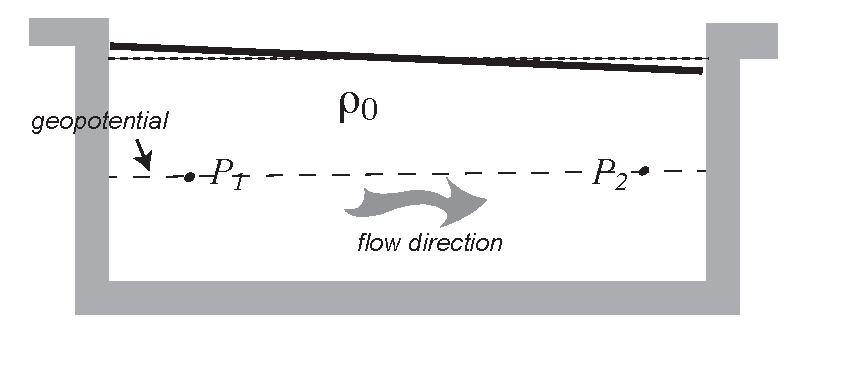
\includegraphics[width=3in]{figs/PdiffSurf}
  \caption{A body of water of uniform density with a tilted upper
    surface.  Note that P1 and P2 are at the same geopotential height (i.e. their value of z is constant)}
  \label{fig:PdiffSurf}
\end{marginfigure}
 
If the sea-surface is tilted, then the pressure will be greater where the sea surface is high than where it is low; in \fref{fig:PdiffSurf}, $P_1>P_2$.  This will drive the flow from left to right.  \emph{Note} pressure increases with depth, so when we think about how the pressure moves water, we need to think about the pressure along a ``geopotential'' surface (ie. a surface along which the water would be flat).  For our purposes, this is a set distance below the flat surface of the water.


In general, it is a good rule to think that the water will move in the direction that will lead to a flattening of the surface.  The resting state of the body of water is to have a flat surface, as indicated with the dashed line at the surface in \fref{fig:PdiffSurf}.  

The situation is more complicated if we add density variations. Consider just tipping the interface of a two-layer fluid (\fref{fig:PdiffTiltInt}). (This is actually hard to do, but just
 imagine).  At first, the pressure difference in the upper layer is zero ($P_3=P_4$) because the upper interface is not tilted.  However, there is more dense water on the left side than the right, so there is a pressure gradient below the interface, $P_1>P_2$, driving deep water to the right.

\begin{marginfigure}
  \centering
  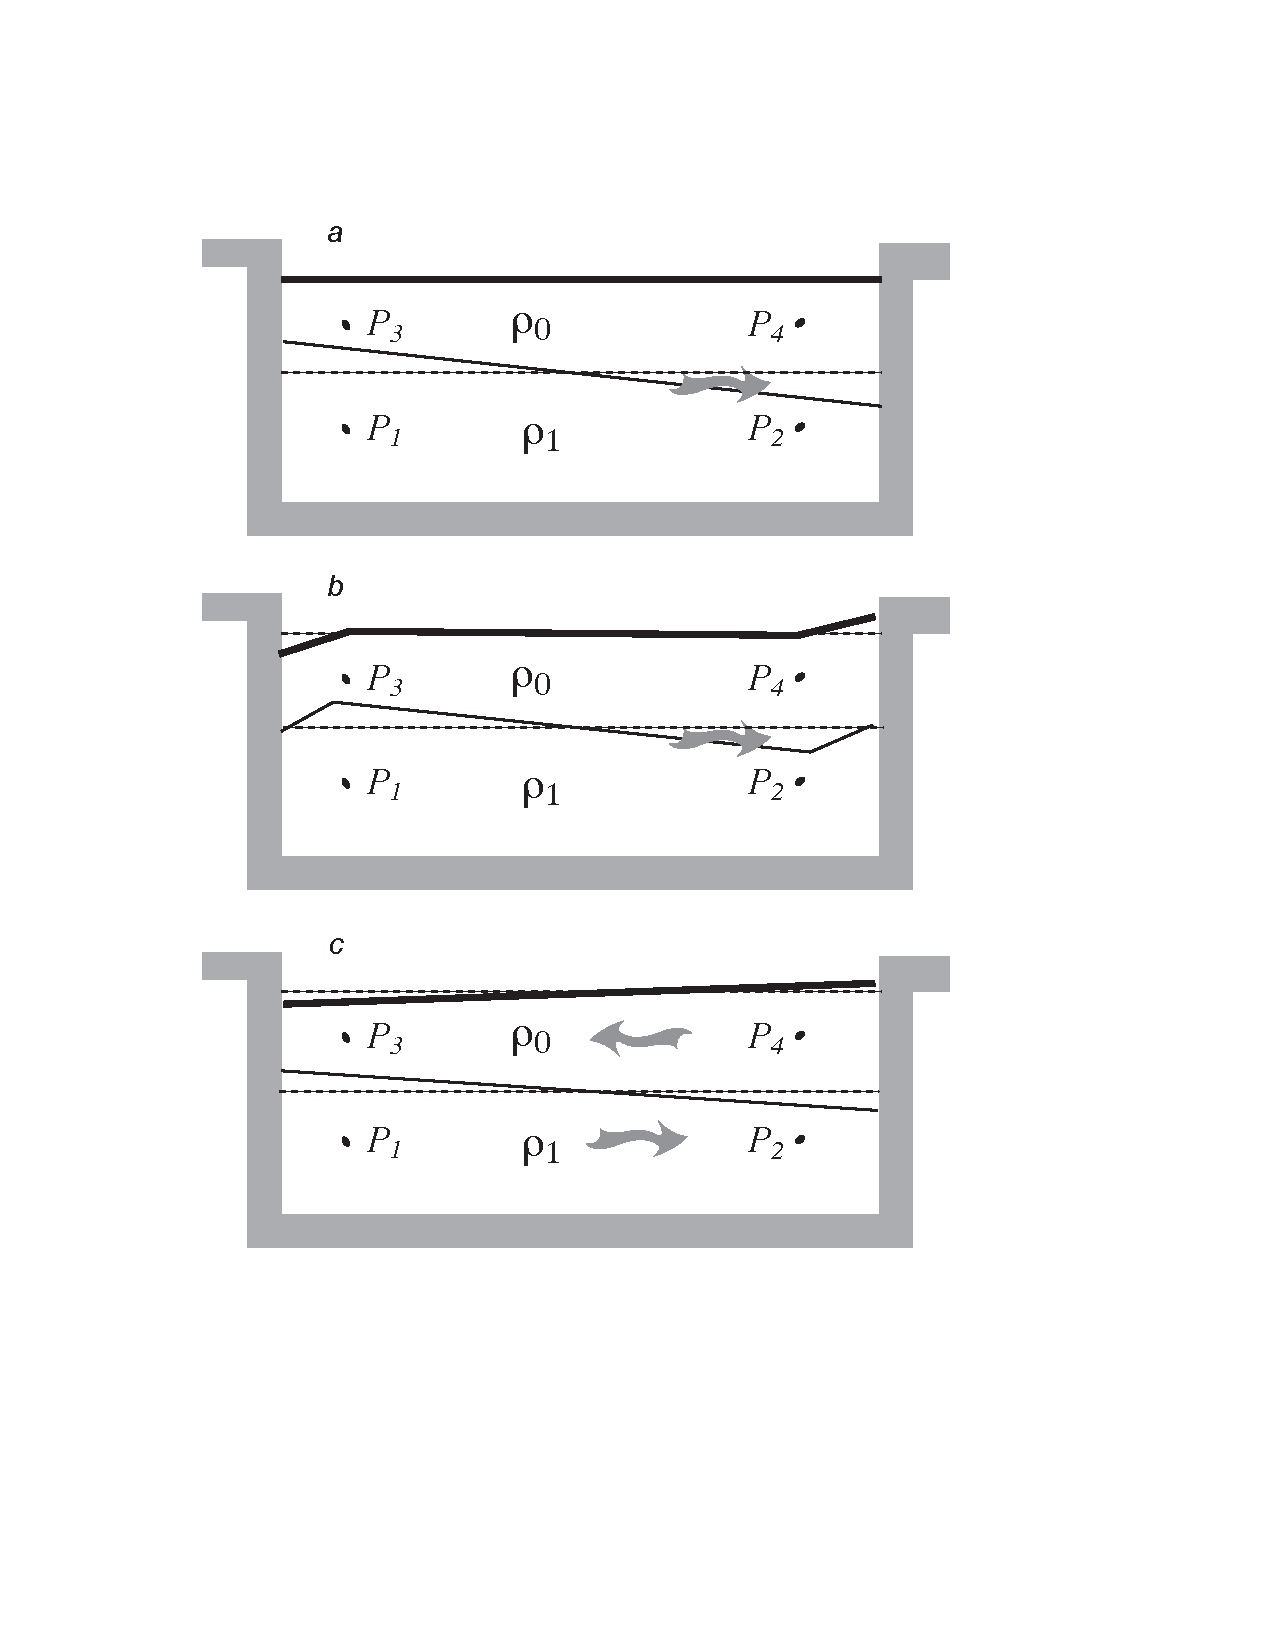
\includegraphics[width=3in]{figs/PdiffTiltInt}
  \caption{A two-layer body water with an interface that is initially
    tilted. See text for the description. }
  \label{fig:PdiffTiltInt}
\end{marginfigure}


This leads to more water, in total, on the right hand side than the left side (\fref{fig:PdiffTiltInt}b).  This makes a surface pressure gradient that tends to drive the upper layer to the left ($P_4>P_3$). This surface pressure gradient is set up \emph{very} quickly, and only involves a tiny amount of water in order to drive the surface-layer flow to the left.

The water column will slosh around for a while, but friction will eventually damp the motions and the interfaces will be flattened as indicated with the dashed lines (\fref{fig:PdiffTiltInt}c).

\begin{marginfigure}
  \centering
  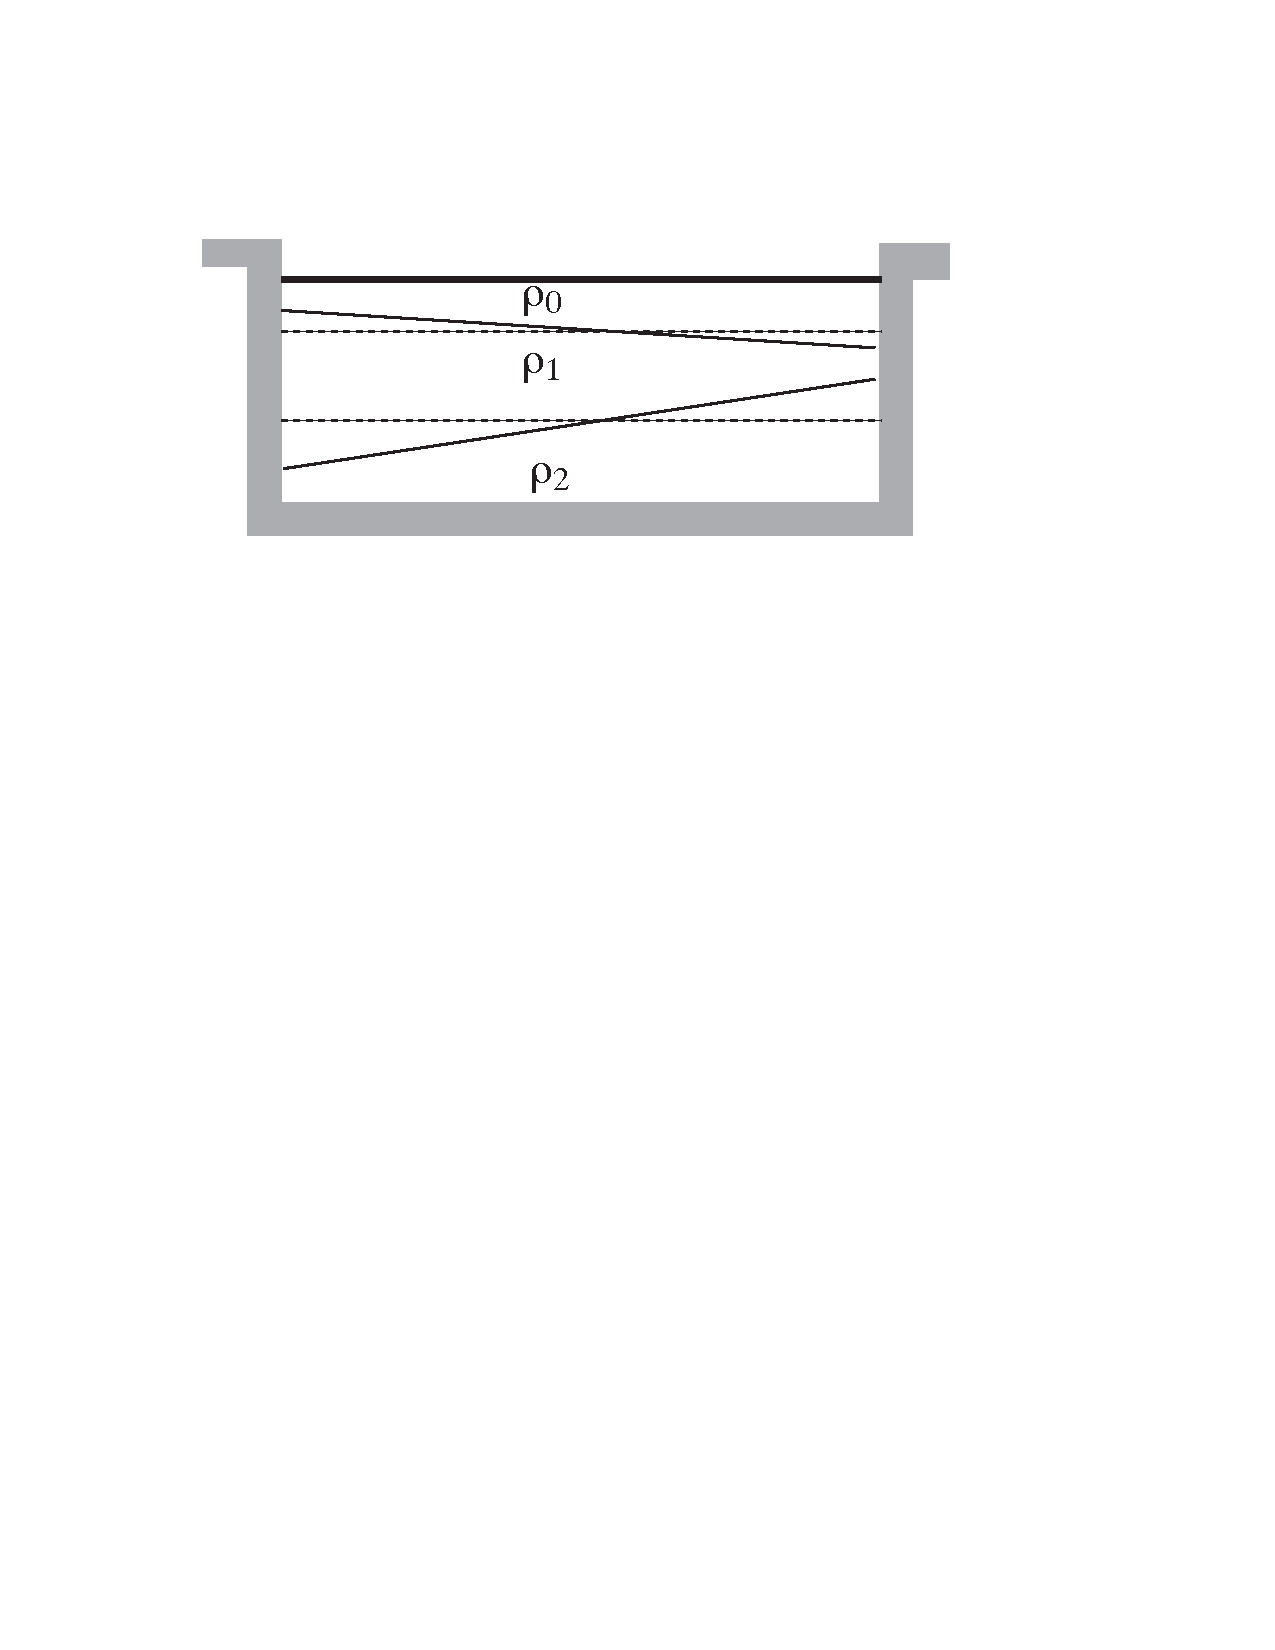
\includegraphics[width=3in]{figs/PdiffTilt3Int}
  \caption{A three-layer body water with tilted interfaces. }
  \label{fig:PdiffTilt3Int}
\end{marginfigure}

Again, the general idea is that the body of water has pressure gradients in it that drive a flow that will tend to flatten the layers.

\studyq{In \fref{fig:PdiffTilt3Int}, what direction does each layer flow?}

\studyq{If the density differences between the layers are equal, which layer will initially have the strongest flow?}


\section{Estuarine Flow}

\subsection{Salt-wedge estuary}

\emph{Estuaries} are bodies of water with opposing buoyancy sources at their ends, usually a river at the head and the ocean at the mouth.  The buoyancy difference usually arise from the salt content of the water, with fresh water being ``lighter'', or more buoyant, than salty water.   The simplest situation is a river spills into the ocean, spreads out and becomes a buoyant plume (\fref{fig:EstuaryNoMix}).  If we quantify the river volume transport as $R$ (typically in units of $m^3\,s^{-1}$) then in \Wikiref{steady state} the transport out the mouth of the estuary will be $Q_o=R$.  The deep ocean layer will be stagnant.

\begin{figure}[htb]
  \centering
  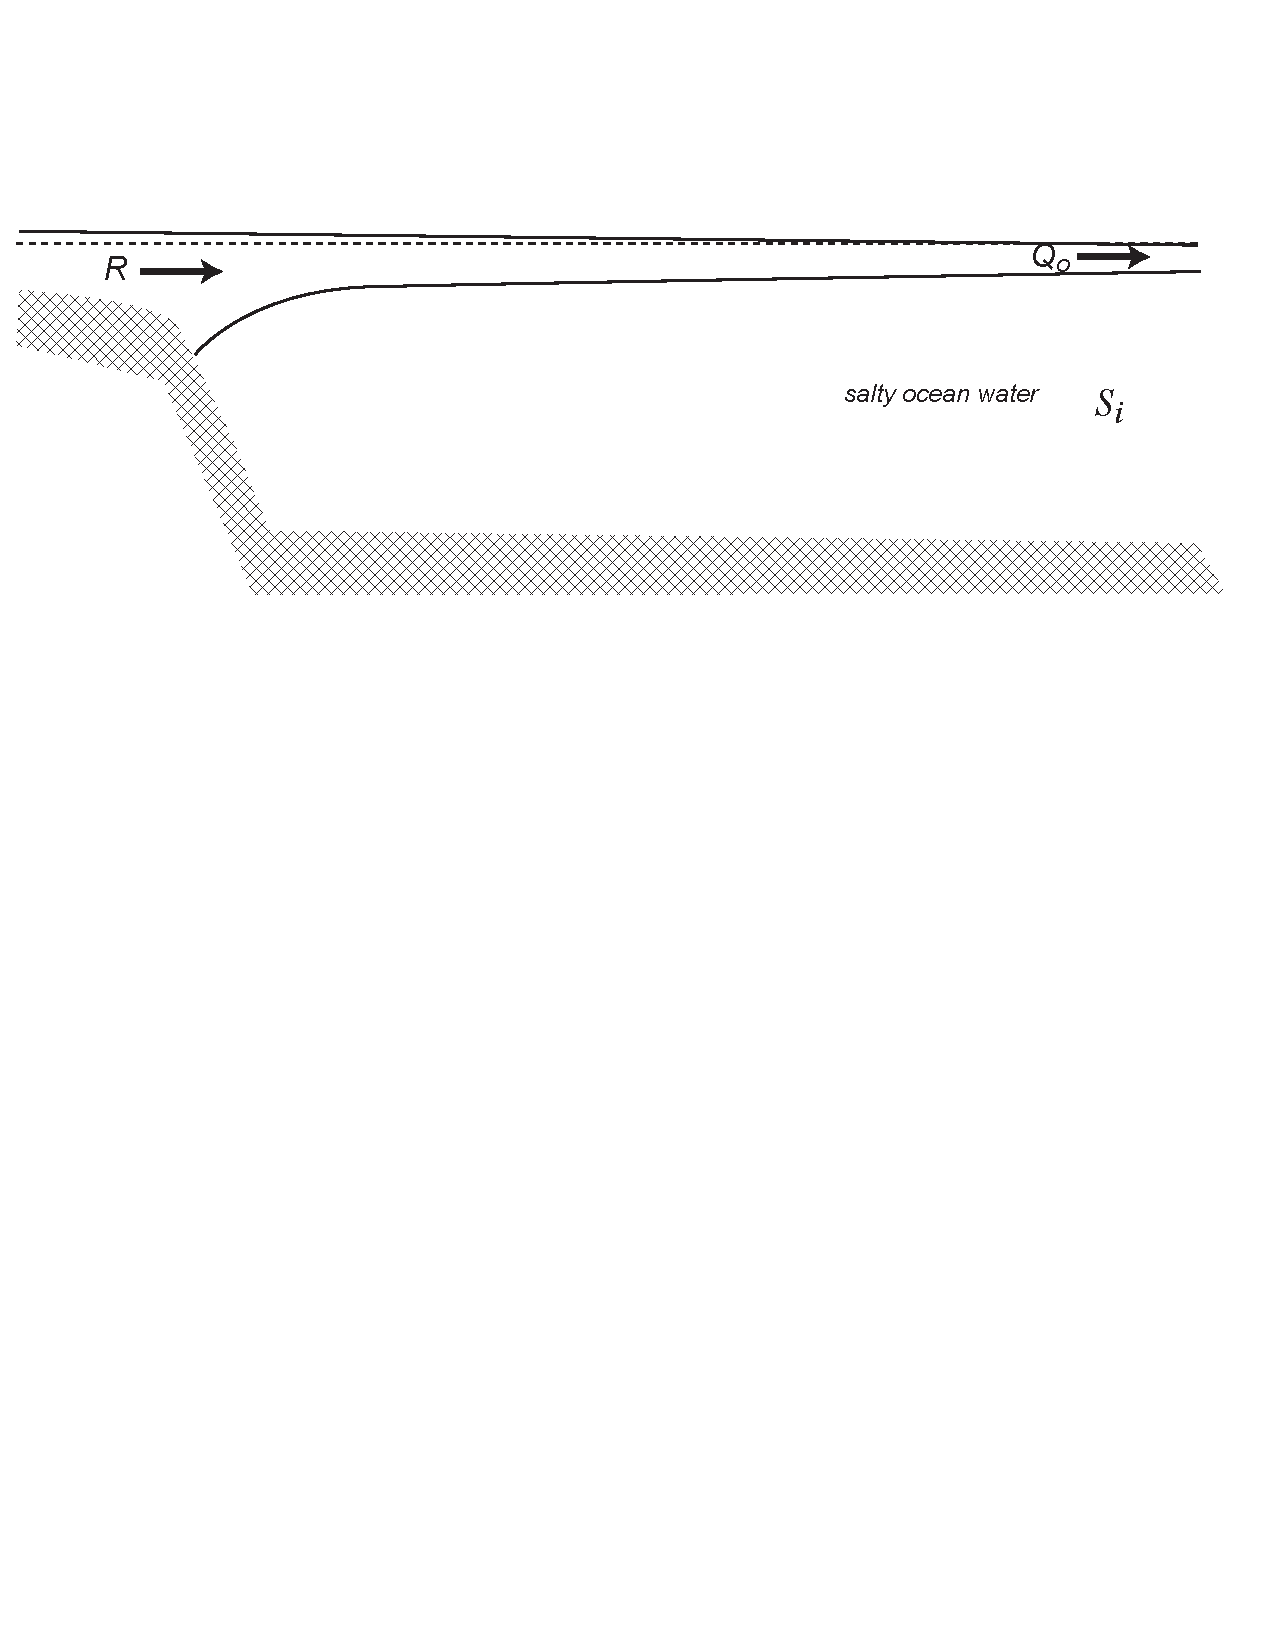
\includegraphics[width=3.5in]{figs/EstuaryNoMix}
  \caption{A salt-wedge estuary and river plume.  The river discharges
    into the salt water without substantial mixing.}
  \label{fig:EstuaryNoMix}
\end{figure}

This type of estuary is called a \emph{salt-wedge estuary}.  The mouth of the Fraser River is a classic example of a salt-wedge estuary with a spreading plume (\fref{fig:GeyerFarmerFig3}).  Fresh water runs over salty with a small amount of mixing between the two layers.  The salinity goes from 2 psu to 24 psu (1 psu $\approx$ 1 part-per-thousand, or gram of salt per kilogram of water) in just a few meters vertically. This sharp front moves back and forth with the tide, a typical feature of most salt-wedge estuaries.

\begin{figure}[htb]
  \centering
  \includegraphics[width=4in]{figs/GeyerFarmerFig3}
  \caption{Salinity contours in mouth of the Fraser River. Salinity has units of parts per thousand, or ppt.  So 1 ppt means 1 gram of salt per kilogram of water. The unit ``psu'' is also often used, meaning practical salinity unit, with $1\ \mathrm{psu}=1\ \mathrm{ppt}$.  The river
    is on the left, the ocean on the right. \citep{geyerfarmer89} }
  \label{fig:GeyerFarmerFig3}
\end{figure}

\subsection{Fjord-type estuary}

Unlike a \emph{salt-wedge} estuary, most estuaries have an ``exchange flow'' that is much stronger than  the river flow.  This flow is driven by vertical mixing that in turn creates tilted ``isopycnals'', or constant density surfaces.  These tilted isopycnals want to slump due to the pressure gradients that are set up, as discussed above.

As an example, imagine the situation pictured in \fref{fig:EstuaryLocal}.  Here a river flows into salty water.  If turbulent mixing is driven by strong tidal flow over the topographic bump in the middle of the estuary, then intermediate-salinity water will be formed.  This intermediate-salinity water will be denser than the river water, but lighter than the ocean water, and will set up a flow that is pictured in \fref{fig:EstuaryLocal}b.

\begin{figure}[htb]
  \centering
  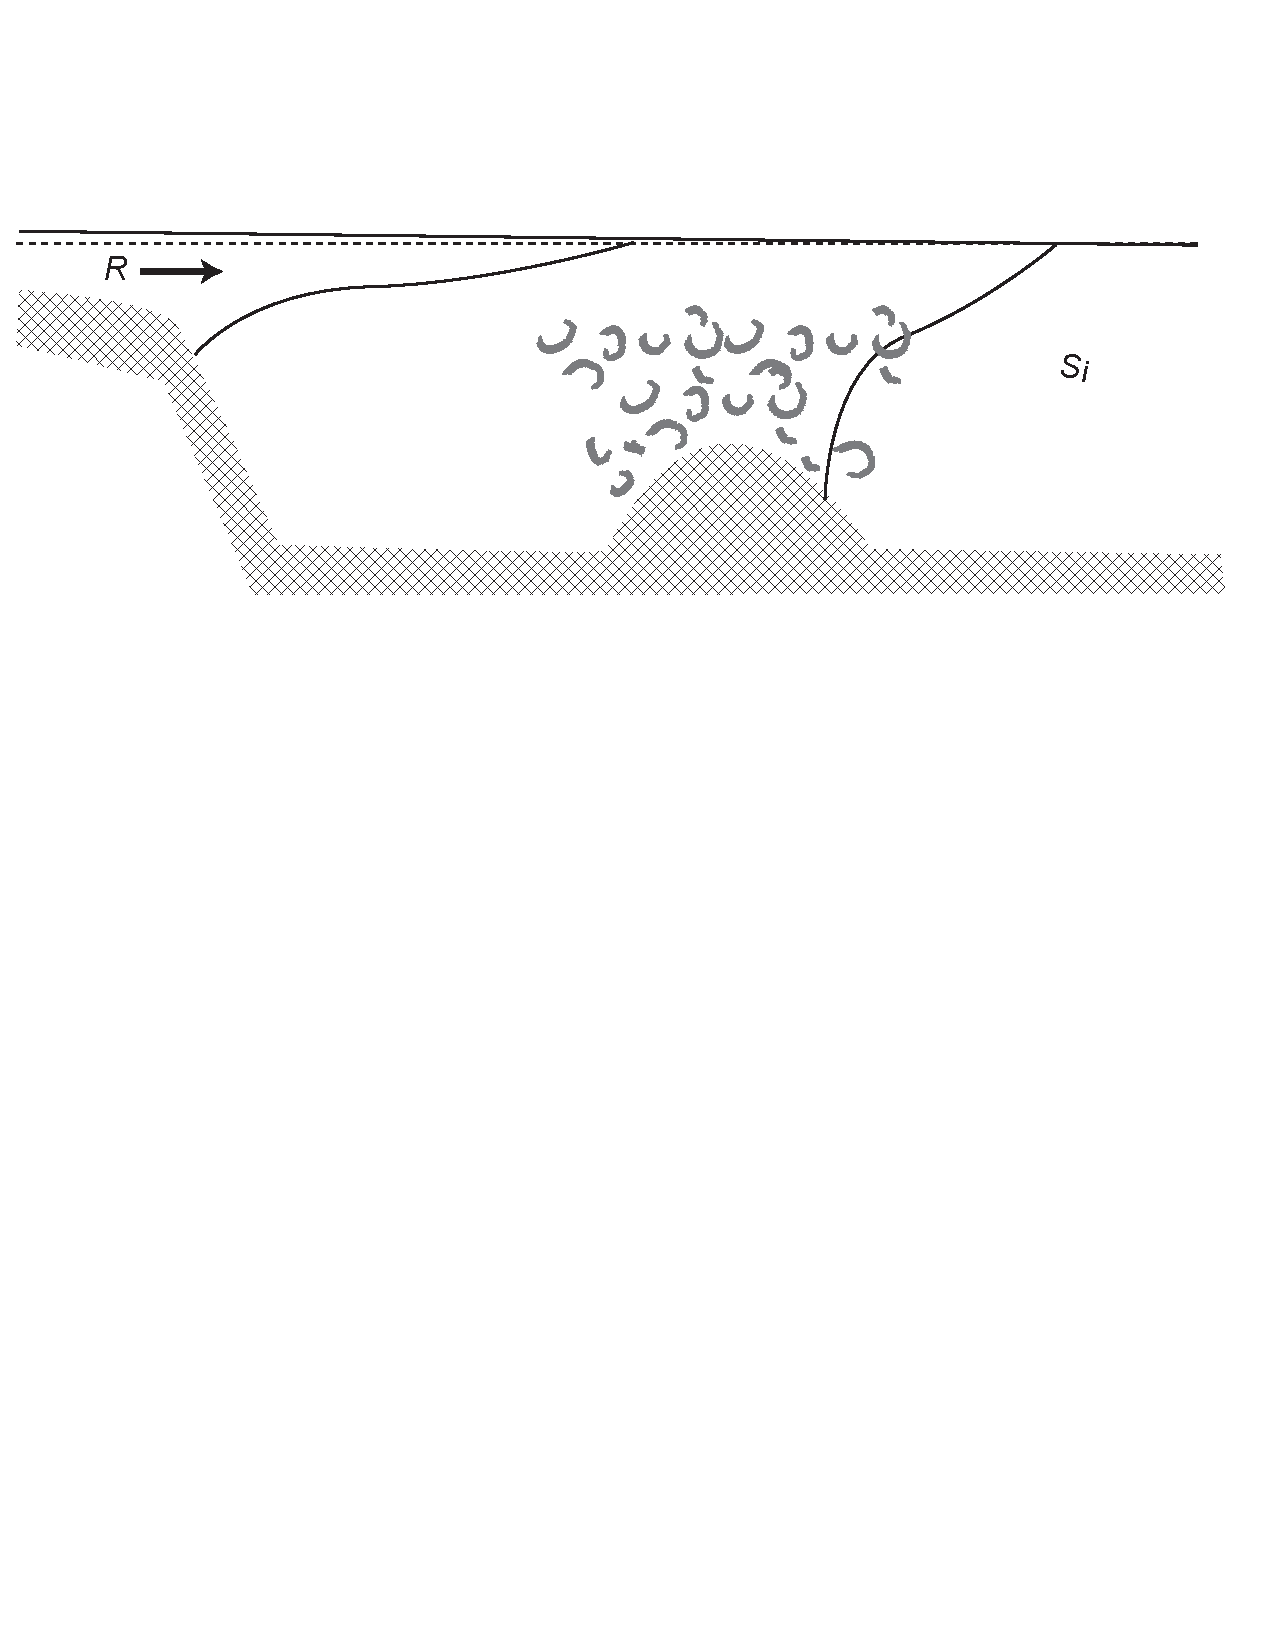
\includegraphics[width=3.5in]{figs/EstuaryLocal}
  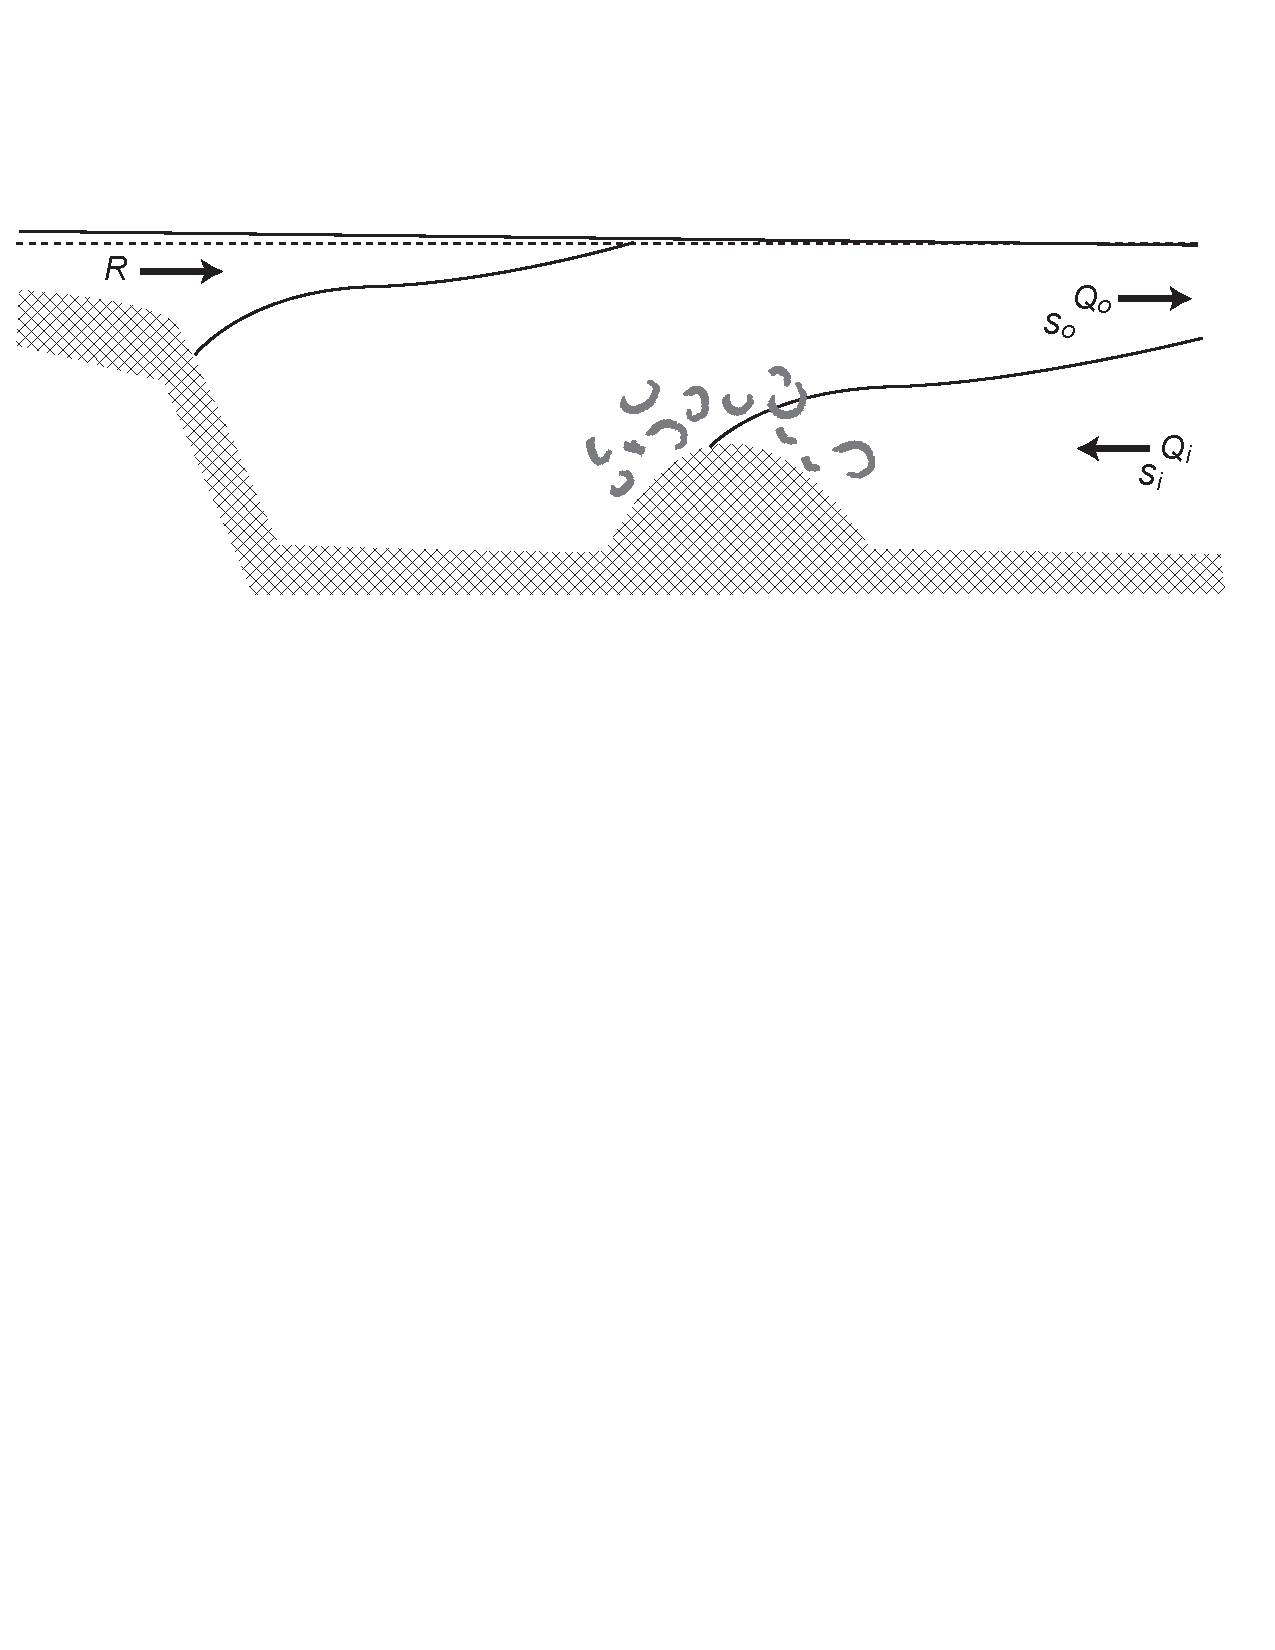
\includegraphics[width=3.5in]{figs/EstuaryLow}
  \caption{The effect of weak local mixing on flow in a fjord-type
    estuary. Intermediate salinity water is formed by the mixing which
  drives a flow out to sea.  In this figure, ``isohalines'' are indicated by the contours (constant salinity surfaces) and will correspond to ``isopycnals'' (constant density surfaces) in most cases.  }
  \label{fig:EstuaryLocal}
\end{figure}

Determining the steady-state for such a flow is not trivial, and not very conducive to theoretical formulation.  However, general tendencies can be determined.  If there is more mixing, more intermediate water is formed. In steady state, this intermediate water must be flushed away, so there is a stronger circulation.  Conversely, if the mixing is weaker, less intermediate water is produced, weakening the circulation.

\subsection{Flood-plain estuaries}

The more mixing that takes place, the more vertical the isopycnals, and the stronger the exchange flow that is driven (relative to the river flow).  The salt and density fields also become much more complicated.  In shallow estuaries, of which the Chesapeake Bay is an excellent example, mixing from bottom stress and the winds tends to affect the whole water column, not just near topographic features.  This sets up large along-estuary salinity and density gradients (\fref{fig:EstuaryHigh}). These types of estuaries tend to have much stronger amplification of the river flow ($R$) because of the extra mixing.

\begin{figure}[htb]
  \centering
  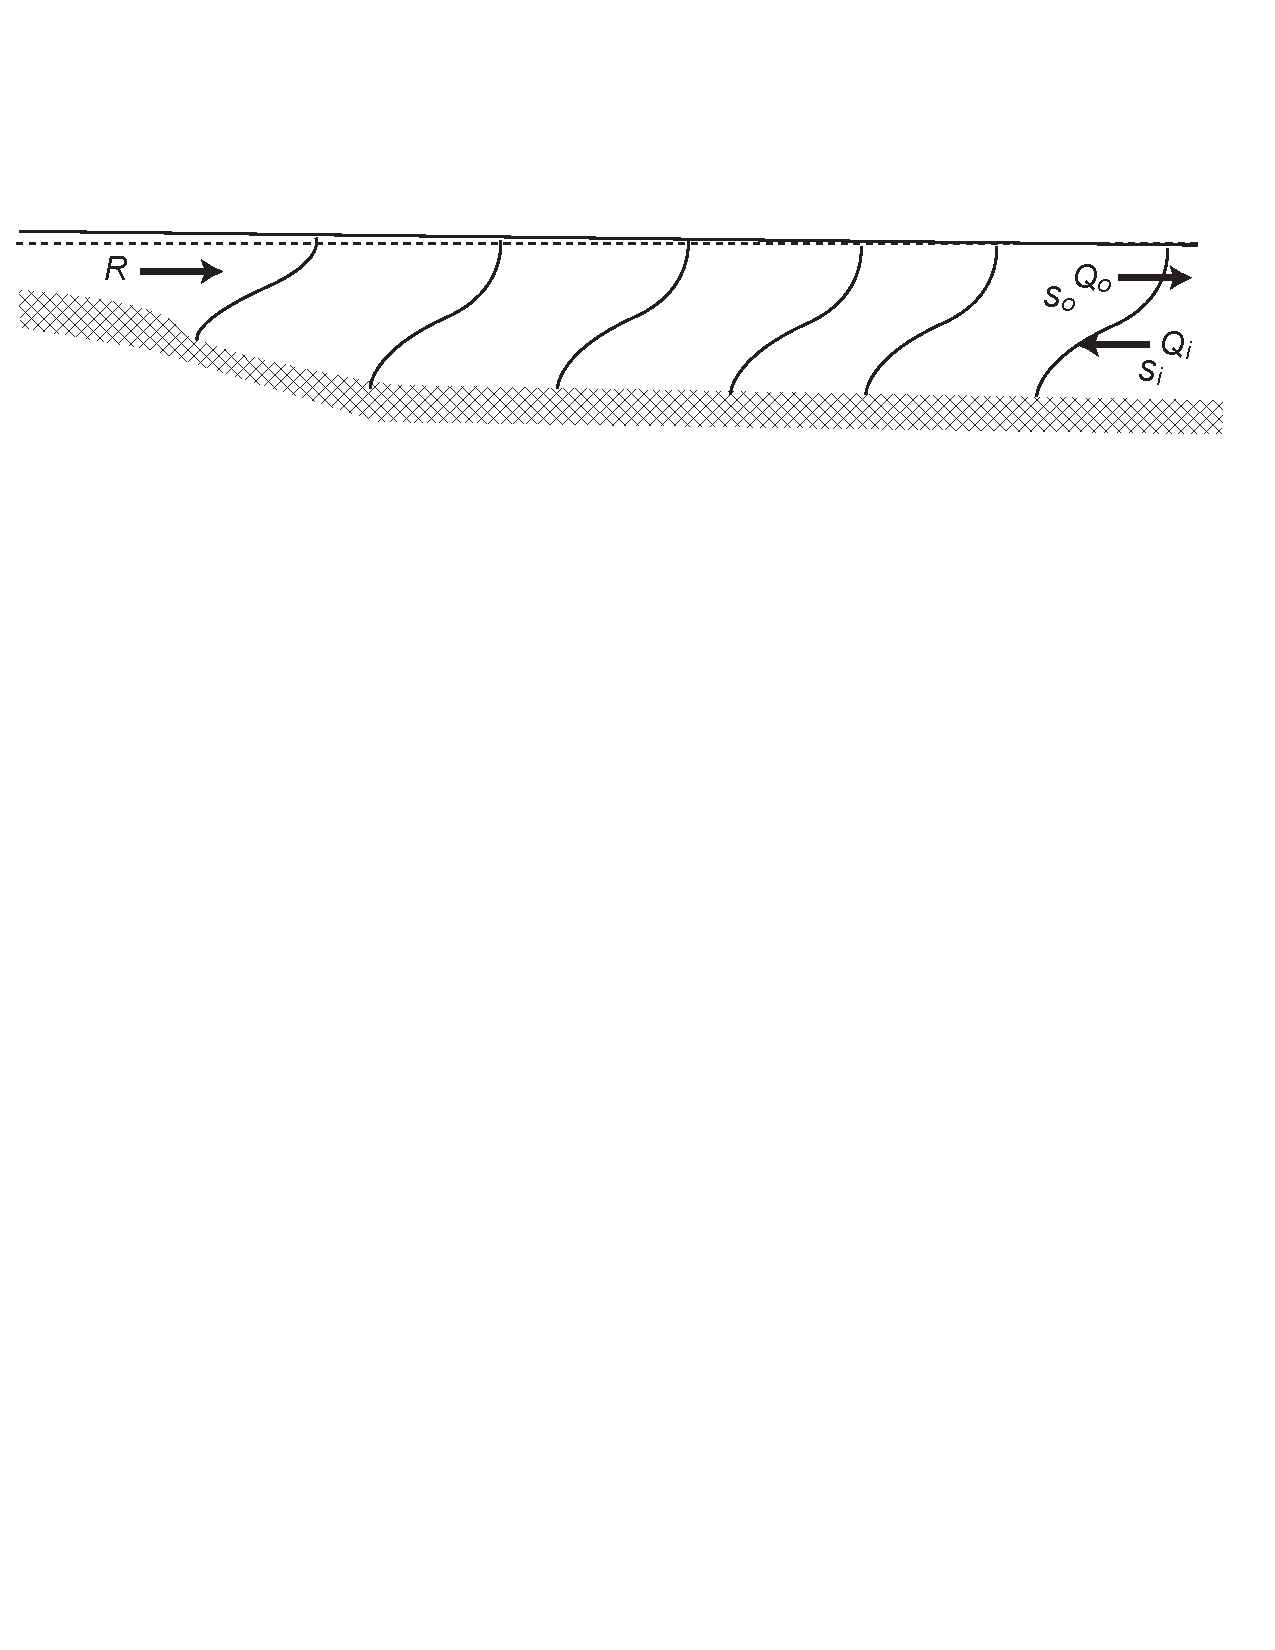
\includegraphics[width=4in]{figs/EstuaryHigh}
  \caption{A flood-plain estuary schematic.  Salinity increases from
    the head to the mouth, with weak vertical gradients.  }
  \label{fig:EstuaryHigh}
\end{figure}


An example from an arm of the Chesapeake demonstrates how such an estuary may look (\fref{fig:Elliott76Fig8}).  Up estuary  of Maryland Point, the estuary is really a river with no salinity.  However, unlike the salt-wedge estuary, there is a gradual horizontal gradient of many kilometers before salty water is found.  Note that even at this point the water is still only 12 psu, and that the Chesapeake Estuary continues for hundreds more kilometers before open-ocean water is found.

\begin{figure}[htb]
  \centering
  \includegraphics[width=4in]{figs/Elliott76Fig8}
  \caption{A salinity cross-section from the Upper Potomac estuary,
    part of the Chesapeake Bay estuarine system \citep{elliott76}.}
  \label{fig:Elliott76Fig8}
\end{figure}

The whole estuary has been measured and simulated numerous times.  A recent example is shown in \fref{fig:LiEtAl05Fig5}.  Here the upper layer of fresher water can be seen flowing south and seaward.  There is a strong return flow in the bottom 20 m.  Note that the volume transport of the return flow is not accurately represented by these velocities, since they do not take into account the fact that the Bay widens considerably as it travels further south.
\begin{figure}[htb]
  \centering
  \includegraphics[width=3in]{figs/LiEtAl05Fig5}
  \caption{A salinity and mean velocity sections from a numerical
    model of the whole Chesapeake Bay \citep{lietal05}}
  \label{fig:LiEtAl05Fig5}
\end{figure}

Also note the lenses of fresher water that appear along the estuary. These occur because of rivers along the length of the estuary. This complicates the simple picture given above, but the general trend of the flow remains unchanged.



\subsection{Time-dependence}

Time dependence changes the steady-state balance in estuaries in three main ways.  First, the fresh-water input at the head of the estuary can change (\fref{fig:SchubelPritchard86}).  This significantly changes the salinity content of the estuary and the estuarine circulation.  Somewhat paradoxically, the increased river flow can lead to a decreased estuarine flow.  For instance in the Apr 1968 panel the isopycnals are much less tilted than in the Oct panel, indicating enhanced flow.  The balance here, however, is not a perfect one, and determining the exact response if the river forcing changes depends on the mixing response.  Strong vertical density gradients caused by fresh water influx can suppress turbulence and hence reduce the mixing required to drive the exchange flow.

\begin{figure}[htb]
  \centering
  \includegraphics[width=4in]{figs/SchubelPritchard86Fig4}
  \includegraphics[width=4in]{figs/SchubelPritchard86Fig5}
  \includegraphics[width=4in]{figs/SchubelPritchard86Fig6}
  \caption{Salinity in the Chesapeake as it varies due to river
    discharge over the year (bars on left) \citep{schubelpritchard86}.}
  \label{fig:SchubelPritchard86}
\end{figure}

A second effect that can change the forcing of an estuary is that  the ocean water at the mouth of the estuary can change salinity due to seasonal changes in the open ocean.  This tends to be a smaller effect because the salinity differences, even in coastal waters, tend to be less pronounced.  However, coastal waters are subject to seasonal changes due to coastal upwelling and downwelling.  During upwelling, denser water can be found at the estuary mouth, whereas during downwelling the density can decrease.

Finally, there is a time dependence to the mixing that ultimately drives the enhanced estuarine circulation.  The most regular source of time-dependence is the tidal forcing. This varies with the fortnightly (every two weeks) modulation of the tide, and with the long-term perigree/apogee variations of the moon-earth-sun system.  More mixing during the \emph{spring} tides leads to \emph{isohalines} that are more tilted (\fref{fig:BlantonEtAl00Fig5}) which therefore drive more circulation.

\begin{figure}[htb]
  \centering
  \includegraphics[width=3in]{figs/BlantonEtAl00Fig5}
  \caption{Salinity in the Mira estuary (Portugal) during neap and spring tides
    \citep{blantonetal00}.}
  \label{fig:BlantonEtAl00Fig5}
\end{figure}

\clearpage
\subsection{Topographic blocking (mostly in fjords)}

One final topic is topographic blocking.  Fjords are often demarcated from the ocean by underwater sills (terminal moraines left over from glaciations).  These sills can be quite tall and sometimes the tides are not strong enough to bring the densest water from the ocean-side of the sill over the sill (\fref{fig:EstuaryBlocking}a).  The estuarine circulation carries on as normal above this depth, but the deep ocean layer does not make it into the landward basin.  This is called ``blocking''.

However, occasionally strong tides perhaps enhanced by atmospheric forcing will conspire to provide enough energy for the densest water to get over the sill.  This dense water will spill over the sill and, if it does not mix, will reach the bottom of the fjord (\fref{fig:EstuaryBlocking}b).  For some fjords this happens every spring-neap cycle.  For others only when the spring tide is particularly large, or the water on the seaward side denser than usual.  

\begin{figure}[htb]
  \centering
  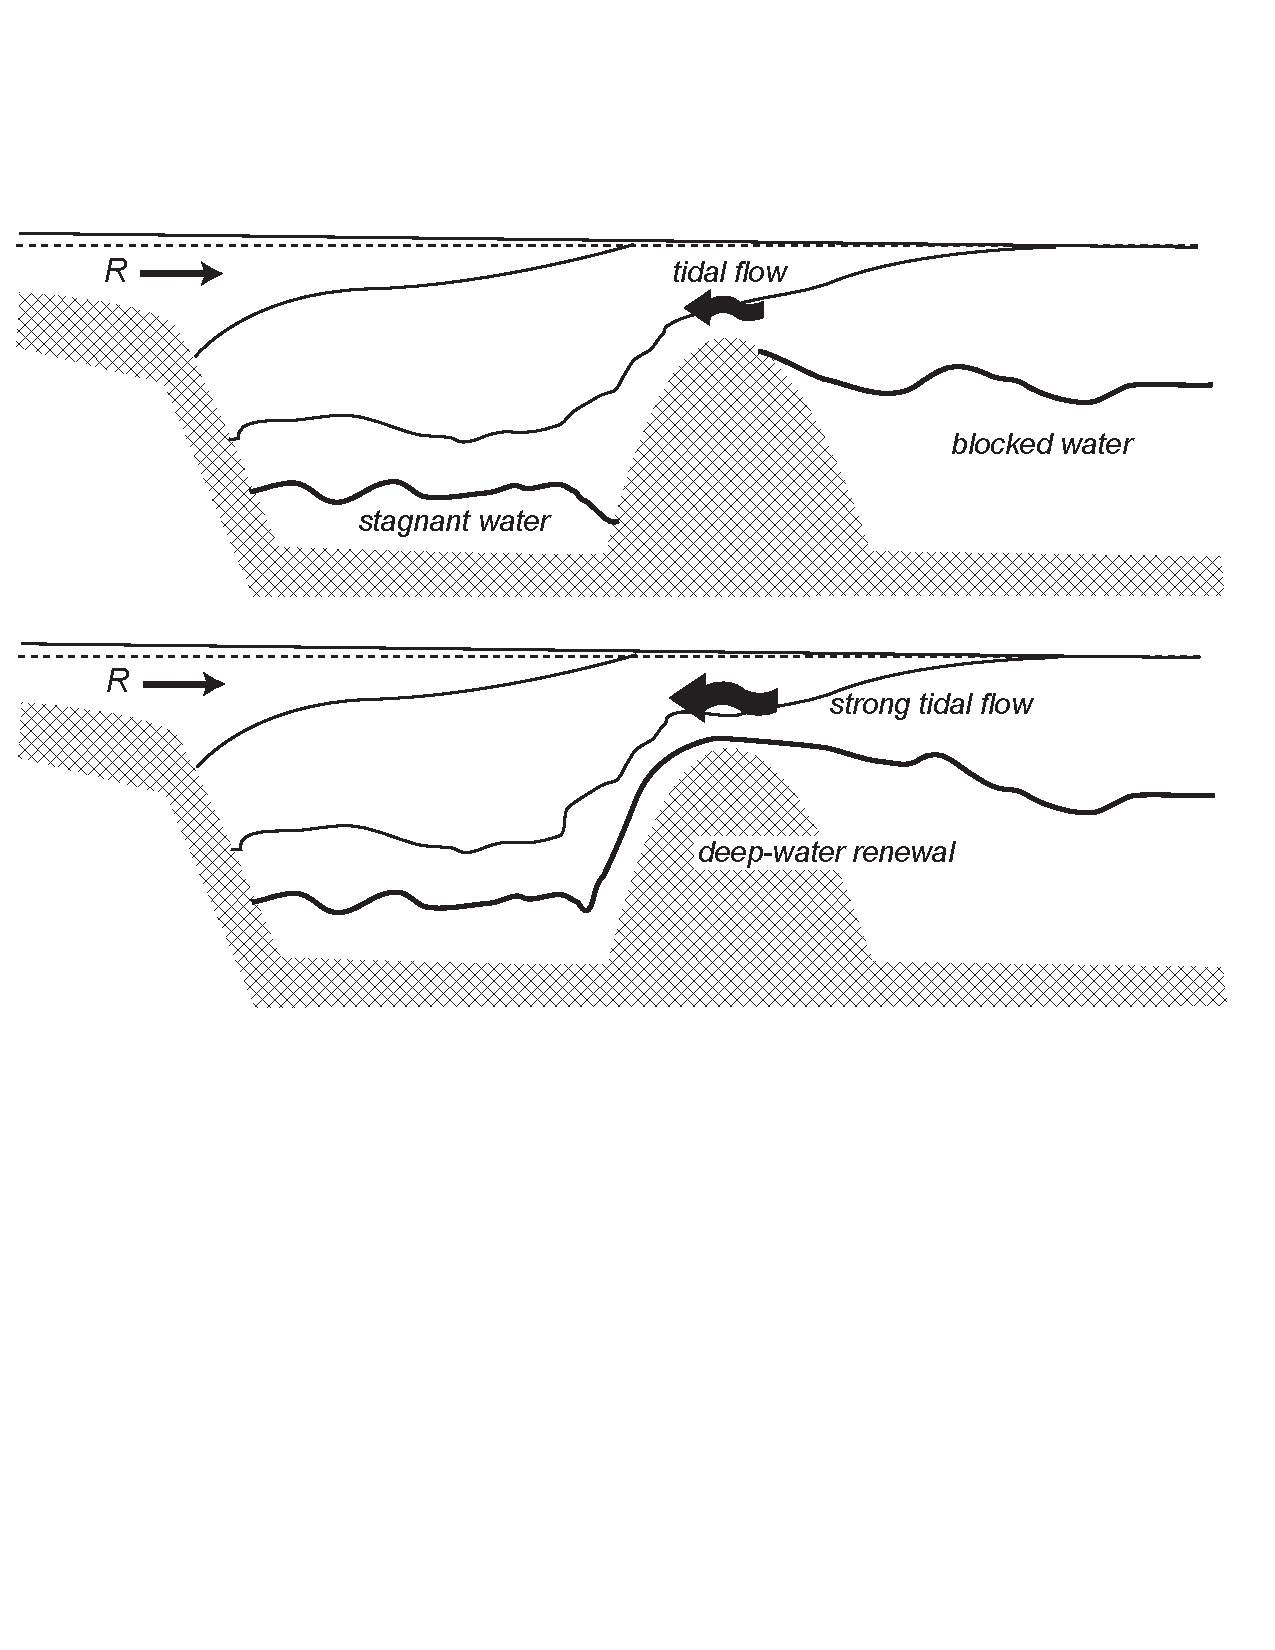
\includegraphics[width=3in]{figs/EstuaryBlocking}
  \caption{A narrow-silled fjord with blocking of deep water, and a
    deep-water renewal event.}
  \label{fig:EstuaryBlocking}
\end{figure}

Conversely, if the sill is broad, or has a lot of horizontal constrictions, deep-water renewal can happen on the exact opposite phase of the spring-neap cycle (\fref{fig:EstuaryBroadSill}).  During spring tides the incoming dense water is subjected to so much mixing that it is mixed away before it can reach the inner basin.  It is only during neap tides with enough velocity to push the dense water into the inner basin, but not so much as to cause excessive mixing that deep-water renewal can take place.

\begin{figure}[htb]
  \centering
  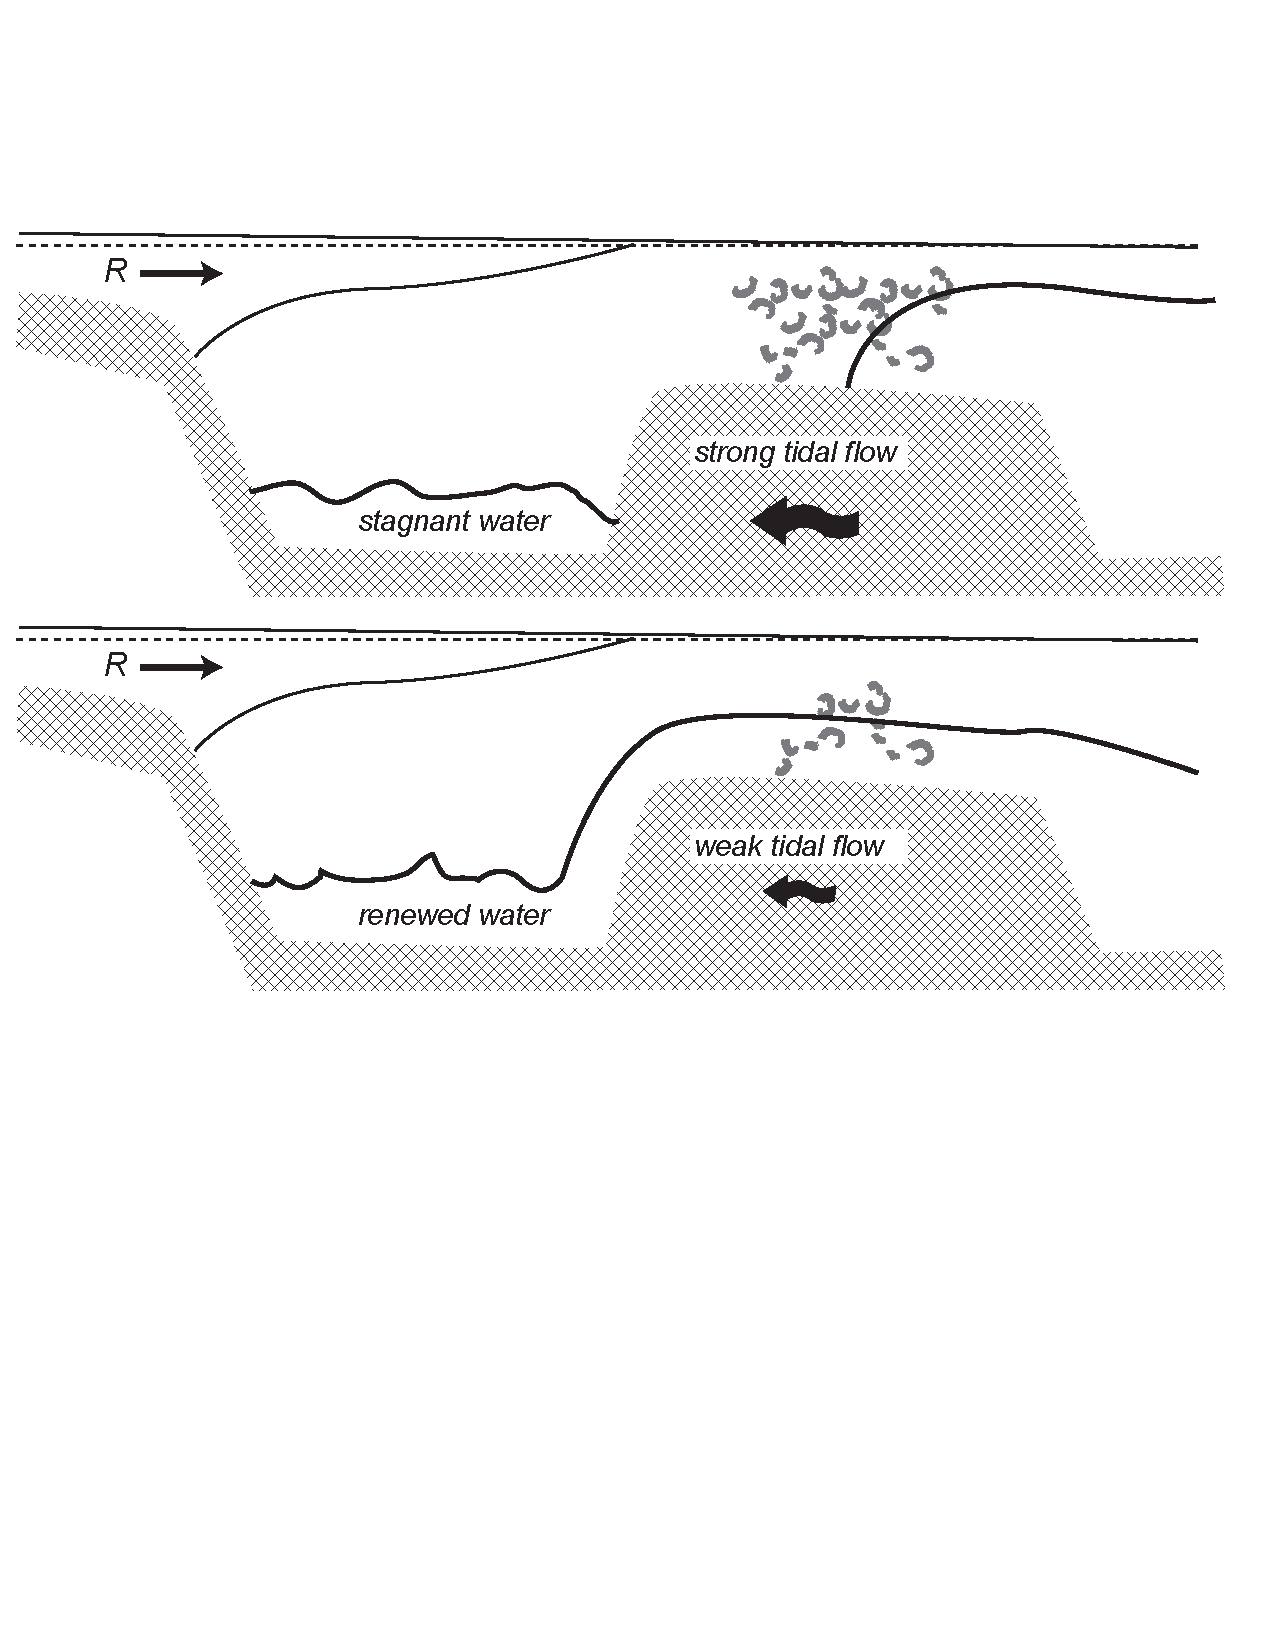
\includegraphics[width=3in]{figs/EstuaryBroadSill}
  \caption{A broad-silled fjord with blocking of deep water during
    spring tides, and a deep-water renewal during neaps.}
  \label{fig:EstuaryBroadSill}
\end{figure}



\section{Quantifying the Circulation}

See also, Open University Sec 6.2

Estuaries are a great example of mass and volume conservation. These concepts are very important for all of oceanography (and probably most of science in general).  Most people are familiar with the concepts, but laying out the mathematics takes some care (often just keeping the units straight!).

In an estuary, water flows in the river mouth, and in and out at the ocean end of the estuary.  If everything is in ``steady-state'' we can write equations that relate the incoming mass of water and mass of salt to the outgoing, and make assumptions about the flow based on those measurements.  The discussion below indicates how that is done.

\subsection{The Conservation of Volume}

Suppose we are interested in the dynamics of a body of water, say a rectangular swimming pool.  The pool has a hose pumping water into it at a rate of volume transport of $q \mathrm{[m^3s^{-1}]}$.  If its surface area  $A$, how fast is the water rising in the pool?

Here the answer is relatively easy.  The speed at which water rises in the pool is $w=q/A$, the volume transport divided by the surface area.  Here we have applied the conservation of volume:
\begin{equation}
  \label{eq:VolCons}
  \frac{\mathrm{d}V}{\mathrm{d} t} = -\sum_i q_i + \sum_j s_j.
\end{equation}
where $V$ is the volume of fluid in the body we are studying, $q_i$ are individual transports out of (positive) or into (negative) the volume.  The last term is the sum of the sources (positive) and sinks (negative) inside the volume, and is included for completeness.  For the conservation of volume of water, a sink could be evaporation, and a source rainfall.  We differentiate such source and sinks from the ``advective'' transports (caused by water velocity) because the physics is distinct.

Formally, this should really be conservation of mass in the volume. In which case:
\begin{equation}
  \frac{\mathrm{d}}{\mathrm{d} t}\int_V \rho \mathrm{d}V  = -\sum_i \rho_i q_i +
  \sum_j \rho_j s_j.
\end{equation}
where the integration over the volume is summing all the mass in the volume.  However, the density of water only changes by a few percent, so \fref{eq:VolCons} is a very good approximation.

\subsection{Calculating volume transport}

Volume transports only arise because water is moving from point a to point b.  Sometimes we are given the volume transport (in $\mathrm{m^3\,s^{-1}}$), but sometimes we want to report the velocity.  i.e. in the swimming pool example above we wanted to know how fast the water was rising (i.e. in $\mathrm{ms^{-1}}$).  In the simple case:
\begin{equation}
  q_i = A_i u_i
\end{equation}
where $A_i$ is the \emph{cross-sectional area} the water is flowing through, and $u_i$ is a velocity \emph{perpendicular} to that area.  In vector calculus we write this as:
\begin{equation}
  q_i = \int_A \mathbf{u}\cdot\mathrm{d}\mathbf{A}
\end{equation}
where the dot product makes it clear that the flux is perpendicular to the area and the integral sign means that we are summing over many small elements.  

\subsection{Conservation of a mass of a substance}

The conservation of a substance (or heat) has essentially the same
terms:
\begin{equation}
  \label{eq:conss}
  \overbrace{\frac{\mathrm{d}}{\mathrm{dt}}\int_VS\,\mathrm{d}V}^{\mathrm{change
    \ of\ amount\ of\ stuff}}= \overbrace{\sum_i q_{S}}^{\mathrm{transport\ of\
  stuff\ in}} +  \overbrace{\sum_j s_S}^{\mathrm{internal\ sources}}.
\end{equation}
Here the substance, $S$, is expressed in stuff-per-volume.
i.e. $\mathrm{g\,m^{-3}}$.  We often discuss the \emph{mean
  concentration in a volume} as $\overline{S} = \int_V S\ \mathrm{d}V
/V$, in which case the equation simplifies to:
\begin{equation}
  V \frac{\mathrm{d}\overline{S}}{\mathrm{d}t} = \sum_i q_{S} + \sum_j s_S
\end{equation}
The \emph{transport} of stuff $q_{S}$ is expressed in units of stuff
per time (i.e. $\mathrm{g\, s^{-1}}$).


\subsection{Using the concentration and volume transport to calculate
  advective transport and flux}

In fluid mechanics we often measure the concentration of a substance
($S$) separately from the volume transport $q$ or velocity $u$.  For
instance if Chlorine is mixed in a vat at a concentration of $S=200\
\mathrm{g/m^3}$ and flows through a pipe at $q_v=0.01\mathrm{m^3 s^{-1}}$
then the rate of chlorine transport into the pool is:
\begin{equation}
  q_S = S q_v
\end{equation}
and has units $\mathrm{gs^{-1}}$.  This is called an \emph{advective transport}
of chlorine.

If instead we knew the velocity of the water $u$ and the
concentration, then we might have expressed this as a \emph{flux} of
chlorine:
\begin{equation}
  F_S = S u
\end{equation}
Because velocity is a vector, this flux is more properly written as a
vector:
\begin{equation}
  \mathbf{F}_S = S \mathbf{u}
\end{equation}
and the flux flows in the same direction as the water.  Note that the
units of the flux are $\mathrm{g\,s^{-1}\,m^{-2}}$.  The \emph{transport} (in g/s) of
the material through an area $A$ perpendicular to the flow is thus simply:
\begin{equation}
  q_S = F_S\,A = S u A.
\end{equation}

This can all get confusing if the concentration is expressed
as parts per thousand, or some other volume unit like that
(i.e. mL/L).  This can be dealt with in the same ways, but it requires
some extra care with the units.

\begin{derivbox}[label={box:examplemass}]{Examples of conservation of mass}

Q: Suppose we have a vat, with volume $V=10\ \mathrm{m^3}$ of water in it.  A hose flows into it at a rate of $0.1\ \mathrm{m^3/s}$ and a second hose flows out at the same rate.  If the concentration of Caffeine in the vat is initially $0 g/m^3$, and $10 g/m^3$ in the hose, what is the rate that caffeine is being added to the tank?

A: it is simply $qC=1 \ g/s$.

Q: What rate is caffeine  leaving the tank initially?

A: The initial concentration in the tank is zero, so $qC=0 g/s$.

Q: Assuming the tank is well mixed, what is the rate of change of the concentration in the vat, initially?

A: This is just the rate of change of the amount of caffeine, $1 g/s$ divided by the volume of water in the vat, so $0.1 g m^{-3} s^{-1}$.

Q: New vat, with three hoses.  One hose has $C_1=10 g/m^3$ of caffeine and flows at $q_1=0.1\ \mathrm{m^3/s}$. The second hose flows in with $C_2=5 g/m^3$, and $q_2=0.4\ \mathrm{m^3/s}$.  If the vat is well-mixed and in steady state, what is the flow out the third hose, and what is the concentration of the caffeine in the water in the vat?

A: First, in steady state, the volume fluxes equal zero (there can be no net flow into the vat), so $q_1+q_2+q_3=0$.  We know $q_1$ and $q_2$, so we know $q_3=-0.5\ \mathrm{m^3/s}$, where the negative sign means water is flowing out.

We also know that there can be no net flow of caffeine, so $C_1q_1+C_2q_2+C_3q_3=0$.  We know everything except for $C_3$, so we solve and get $C_3= \frac{C_1q_1+C_2q_2}{-q_3}= 6 g/m^3$.

\end{derivbox}

\subsection{Application to Estuaries: the Knudsen Relation}

An application to estuaries is to conserve both volume in the estuary,
and salt.  Imagine that the flow at the mouth is two layers, one in with a
volume transport $Q_i \ \mathrm{m^3 s^{-1}}$, and one out with volume transport $Q_o$, and
that the river has a volume transport of $R$.  Suppose the salinity of
the lower layer flowing in is $S_i$ in units of parts-per-thousand,
and the salinity of the layer flowing out is $S_o$.

\emph{Q: What is the salinity of the river?}

\emph{Q: What is the salt transport into the fjord in $\mathrm{g/s}$?}

\emph{Q: Assuming the fjord is in steady state, write out an equation
  for the volume budget, and a second equation for the salt
  budget. i.e the volume transport in equals the volume transport out and the
  salt transport in is equal to the salt transport out.}

\emph{Q: Assume $R$, $S_i$, and $S_o$ are known.  Show that:
\begin{equation}
  \label{eq:knudsen}
  Q_i = \frac{S_o R}{S_i-S_o}.
\end{equation}
}

\emph{Q: If there is no mixing of the river water, what is $S_o$, and how big is $Q_i$?}

\emph{Q: If there is lots of mixing, what happens to $S_i-S_o$ and
  thus $Q_i$?}


\clearpage
\section{Exercise}

We will practice some of what we have learnt based on a paper about
local waters by \citet{massoncummins04}. As part of your final project
you will read about similar processes in Saanich Inlet
\citep{gargettetal03}.

{\bf Q:}  Consider \fref{fig:MassonCummins04Fig6}, which shows the
salinity observed and modeled in the Strait of Juan de Fuca.  Based on
these plots, where do you think the mixing is the strongest in the
Strait?

\begin{figure}[htb]
  \centering
  \includegraphics[width=4in]{figs/MassonCummins04Fig6}
  \caption{Observed and modeled salinity in the Straits of Juan de
    Fuca and Georgia \citep{massoncummins04}. The ocean is on the left, and the Fraser River is at Distance = 270 km. The upper plot (a) are the observations and the lower (b) a numerical simulation. }
  \label{fig:MassonCummins04Fig6}
\end{figure}

{\bf Q:}  For the flow in \fref{fig:MassonCummins04Fig6}, sketch where you think the water is flowing.  What happens north of the Fraser river (at Distance = 250 km; make sure you know where north is on this plot)?

{\bf Q:} Consider \fref{fig:MassonCummins04Fig15}, which compares two numerical model runs, one with tides and one without.  Which is which, and why?  Which has the stronger horizontal circulation?

\begin{figure}[htb]
  \centering
  \includegraphics[width=4in]{figs/MassonCummins04Fig15}
  \caption{Salinity for two model runs, one with and the other without
    tides \citep{massoncummins04}. }
  \label{fig:MassonCummins04Fig15}
\end{figure}

\textbf{Q:} A seasonal time series of the salinity in Haro Strait is given in \fref{fig:MassonCummins04Fig10}.  What features of the flow can you identify that indicate the time dependence of the estuarine flow?  Pay particular attention to the modeled timeseries (which has better temporal resolution)?

\begin{figure}[htb]
  \centering
  \includegraphics[width=4in]{figs/MassonCummins04Fig10}
  \caption{Time evolution of observed and modeled salinity in Haro
    Strait \citep{massoncummins04}. }
  \label{fig:MassonCummins04Fig10}
\end{figure}

\textbf{Q:} Use the Knudsen relation on the two data plots in
\fref{fig:MassonCummins04Fig15} to \emph{estimate} the exchange flow if the
river input is $10^4\ \mathrm{m^3\,s^{-1}}$.  Which case has a
stronger exchange, a) or b)?

\textbf{Q:} Suppose the river is suddenly damned, so $R=0 \ \mathrm{m^3\,s^{-1}}$.  The estuary's average salinity will (initially) change at what rate (in units of $\mathrm{psu\,s^{-1}}$)?  Hints: first, you should assume that the estuary adjusts so the flux in is equal to the flux out the mouth.  Second, you need to estimate the volume of the estuary to answer this questions.  Rough numbers are fine, based on the figures above.

\clearpage
\begin{derivbox}[label={box:practicevolume}]{Practice questions (not the exercise!)}

Some students are not comfortable with volume and mass balances.  If
that is the case, try some extra practice questions below. Please ask
me if you need more help with these!
\begin{itemize}
    \item Suppose the water level of a straight-sided pool is observed to rise
at 0.01 m/s, and has a surface area of $50\ \mathrm{m^2}$.  There is one
hose filling it with speed 4 m/s and cross-sectional area $0.01 \mathrm{m}^2$,
and a second hose filling it with a cross sectional area of $0.02 \mathrm{m}^2$.
What is the flow speed in the second hose?
    \item Suppose a pipe has a diameter of 0.1 m and a flow speed of 1 m/s.  If the pipe narrows to 0.05 m what is the flow speed at that part of the pipe (in steady state)?
    \item Suppose there is a vat with $200\ \mathrm{g/m^3}$ solution of chlorine being fed into the pool through a hose with diameter 0.1 m at a rate fast enough to replace evaporative losses in the pool of $0.01\ \mathrm{m^3/s}$.  What is the transport of chlorine into the pool?
    \item If the average concentration of chlorine in the pool is initially $50\ \mathrm{g/m^3}$ and 1000 s later is measured to be $55\ \mathrm{g/m^3}$, what is the volume of the pool?
\end{itemize}







\end{derivbox}
%%% Local Variables:
%%% mode: latex
%%% TeX-master: t
%%% End:

% todo: add study questions
% todo: add exercises
% \documentclass[12pt, oneside]{book}

\chapter{Equation of State and Pressure Gradients}
\label{chap:EquationofState}

In this chapter we go back now and consider some fundamentals about water that are important to this course.  Seawater is a relatively complex substance.  As discussed before, lateral density differences can drive lateral circulation, hence it is important to understand and predict how those differences arise.  Further, the ocean is a huge reservoir of heat, and understanding its heat content is important for predicting weather and future climate.

\section{Temperature}

Temperature is a thermodynamic property of a substance, the value of which is proportional to the kinetic energy of the random motions of the molecules in the substance (these are called \Wikiref{Brownian motion}). The heat necessary to bring a substance to a given temperature is proportional to the \emph{\Wikiref{heat capacity}}.  In order to change a parcel of water's temperature by $\Delta T$, we need to supply energy proportional to the heat capacity of the water:
\begin{equation}
   \Delta E = c_p\ \Delta T
\end{equation}
where $c_p$ has units of $J\, C^{-1}\ kg^{-1}$, and $\Delta E$ has units of $J\ kg^{-1}$.  Values for $c_p$ are given in \fref{fig:HeatCapacity}, and note that the heat capacity is not constant, but depends on the temperature of the water, its salinity, and its pressure!  The dependence is non-linear, so we usually resort to using a computer to calculate the empirically-derived values.  However, for a litre of fresh water ($\approx 1\ kg$) at $20^oC$ we would need 4180 J of energy to raise the temperature by one degree.  

\begin{figure}
    \includegraphics[width=3in]{./figs/HeatCapacity.pdf}
    \caption{Heat capacity of water a) for fresh water as a function of temperature, b) as a function of both salinity and temperature.  Both are presented at the sea surface.}
    \label{fig:HeatCapacity}
\end{figure}

The heat capacity of water is impressive compared to air, where typical values are $1000\ J\, C^{-1}\ kg^{-1}$.  The whole atmosphere has a weight of $\approx 10^{4} \ kg\ m^{-2}$, so heating the whole atmosphere one degree requires $\approx 10^7 J\ m^{-2}$.  Conversely, the ocean at 4000 m deep and with a density close to $1000 \ kg\,m^{-3}$ weighs approximately $4\times10^6\ kg\ m^{-2}$, so raising its temperature by one degree requires $16\times10^9 J\ m^{-2}$, more than three orders of magnitude more energy.  This helps explain why the ocean is such an important reservoir of heat in the climate system.  

\subsection{Measurement}

\begin{figure}[hbtp]
  \begin{center}
    \includegraphics[width=1in]{figs/CTD.pdf}
    \includegraphics[width=3in]{figs/ThermistorConductity.pdf}
    \caption{a) CTD b) thermistor and conductivity probe on a CTD.}
    \label{fig:CTD}  
  \end{center}
\end{figure}

Temperature is measured in the ocean by thermometers.  The typical technology is what is called a ``\Wikiref{thermistor}'', which is a metal in which the electrical resistance changes proportional to its temperature.  Since its relatively easy to design an electronic circuit to measure resistance, this has allowed rapid and automatic measurement of ocean temperatures since such thermistors were first developed in the 1970s.  

Once calibrated, quality ocean thermistors are typically accurate to $0.001\ ^oC$, and are stable to similar levels. It takes time for the thermistor to respond to temperature changes in the ocean, so designing the sensors is a tradeoff between physical robustness and response time.  Typical response time is about 0.3--0.5 s, which is quite fast for ocean changes, but can be slow relative to a CTD being lowered in the ocean. 

\subsection{In-situ and potential temperature}
\label{sec:potential-temperature}

Ocean temperatures are largely set at the sea surface either by absorbing sunlight or exchanging heat with the atmosphere, and subsequently modified by ocean mixing.  The temperature of the water is thus a powerful \emph{tracer} of where a water mass last saw the surface of the ocean, with warmer waters found near the equator, and colder near the poles.    


However, the effect of pressure on the temperature makes it harder to trace where water came from.  The temperature of a water parcel that is moved from one depth to a deeper one will increase because the pressure has increased, even if no heat is exchanged with its surroundings during the move (we call this an \emph{\Wikiref{adiabatic process}}).  A thermistor will measure this change. If the parcel is \emph{adiabatically} brought back to the original depth, its temperature will drop again.  

In order to remove this adiabatic heating effect, its useful to differentiate between the actual \emph{in-situ} temperature and instead report the \emph{potential temperature}.  This is simply the temperature the water would be if it was brought adiabatically to the surface.  

The reason for doing this is dramatically illustrated by considering the temperature measured in the Kermadec Trench \citep{Warren73}.  The trench is much deeper than the surrounding water, so water in the trench has been there a long time.  However, the in-situ temperature increases with depth which might make us think either it is different water, or that there is a heating source from below (\fref{fig:Trench}, curve labeled with "t").  However, computing the \emph{potential temperature} $\theta$ shows that this water is the same potential temperature (\emph{isothermal}) deeper than 5000 m.   

\begin{marginfigure}
\begin{center}
  \includegraphics[width=2in]{figs/Trench}
  \caption{CTD data from Kermadec Trench \citep{Warren73} \emph{in situ} temperature and potential temperature. (Figure from \href{http://oaktrust.library.tamu.edu/handle/1969.1/160216}{Stewart})}
  \label{fig:Trench}
  \end{center}
\end{marginfigure}

Outside of the deepest part of the ocean, the difference between potential and in-situ temperatures are not large (\fref{fig:P16Temp}).  In the deepest ocean, its clear that the cold tongue of water that originates in the Antarctic Circumpolar Current originates shallower in the water column than we would infer from just looking at the \emph{in-situ} temperature.  This improved ability to trace the source of water without accounting for pressure effects is the main motivation for using potential temperature, and most publications will use potential temperature exclusively.  

\begin{figure}[hbt]
  \begin{center}
    \includegraphics[width=5in]{./figs/P16Temp.pdf}
    \caption{North-south sections in the Pacific ocean at a longitude of 150 W, plotted as the measured \emph{in-situ} temperature (upper panel) and the potential temperature, $\theta$ (lower panel).    }
    \label{fig:P16Temp}  
  \end{center}
\end{figure}

\section{Salinity}

Salinity is the measure of dissolved solids in seawater, and is expressed as grams of solids per kilogram of seawater.  Because it is derived from solids in the seawater, salinity is hard to define, and quite hard to accurately measure in the ocean. Oceanographers are greatly aided by the fact that the residence time of a salt ion is very long compared to the mixing timescale of the ocean.  While we think of rivers as being composed of fresh water, the input of salt ions largely come from the trace amounts in these rivers. In total, there is $\approx 5 \times  10^{19}\ kg$ of salt in the ocean, but inputs are $\approx 2.5 \times  10^{12}\ kg/year$, so the \emph{\Wikiref{residence time}} of salt in the ocean is around 20 million years.  The overturning time scale of the ocean is 3000 y (at the most), so salt in the ocean is ``well-mixed''. This long residence time means that the ratio of salt constituents in the oceans only changes on geological time scales, and thus in the open ocean the ratio of various ions can be considered a constant (closer to river sources the ion ratios can be quite different).  

Note, however, that the ratio of the solids that make up the salt being constant does not mean that \emph{salinity} itself is constant.  The concentration of salt in a given volume of water depends on how much river water or rain water that parcel has been in contact with, or if it has been subject to evaporation.  

\subsection{Measurement}

Chemical oceanographers spent many decades studying the chemical makeup of salt water.  The standard way of measuring salinity was to titrate the chloride solids and then use the fact that the ratio of salt ions in the ocean is relatively constant to infer the total salinity.  This is done more rarely now, and instead oceanographers measure the \emph{conductivity} of  seawater using a conductivity cell. This uses the fact that salt water conducts electricity better than fresh water, and thus the amount of electricity thats able to get from an electrode to an anode through a known quantity of seawater is proportional to the conductivity. 

Electric circuits to measure conductivity are relatively straight forward, but the most stable measurements require a good-sized sensing sensing element over which to take the measurement.  The conductivity cell in the CTD shown in \fref{fig:CTD}a is about 15 cm long to allow a stable and accurate estimate.  This means that there is a limitation to how fine the vertical resolution of the conductivity estimate is.

\begin{marginfigure}
\begin{center}
    \includegraphics[width=2.2in]{./figs/Conductivity}
    \caption{Conductivity as a function of temperature and salinity}
    \label{fig:Conductivity}
\end{center}
\end{marginfigure}

The largest challenge in measuring salinity using conductivity is that conductivity is also a strong function of temperature as well as salinity (\fref{fig:Conductivity}).  That means that we need to have a well-matched temperature measurement at the same time and place as the conductivity measurement in order to back out the salinity.  Mismatched sensors lead to a phenomena known as "salinity spiking".  It is easily understood if we consider measuring through a temperature interface in water that  has a uniform salinity (\fref{fig:SalinitySpike}).  If the temperature sensor is lagged compared to the the conductivity sensor, the conductivity will go down, but the temperature measured by the temperature sensor will not until a deeper depth.  When the salinity is calculated from these two measurements, there will be a sharp discontinuity in inferred salinity at the interface because the sensors are not matched up. This is a very hard problem to get rid of, and involves making sure the two sensors are not lagged from one another, and making sure that their signals are smoothed enough that the mismatch in how the sensors respond to changes are smoothed over.  

\begin{figure}[hbt]
  \begin{center}
    \includegraphics[width=4in]{./figs/SalinitySpike.pdf}
    \caption{Salinity spiking due to conductivity and temperature sensors not being aligned; here the temperature sensor lags the conductivity sensor, so the cold change with depth is registered in the conductivitsy sensor before the temperature. Note the conductivity change is completely due to temperature.}
    \label{fig:SalinitySpike}
  \end{center}
\end{figure}

Regardless of measurement issues, the measurement of salinity using conductivity and temperature is very wide spread.  In order to differentiate such measurements from fundamental chemically based estimates, oceanographers often use the units of "practical salinity units" or "psu".  When these units are used, the measurement is almost always from a CTD.  More recently, there is a new salinity unit used as part of an update to the equation of state (\href{www.teos-10.org}{TEOS10}), where salinity is denoted as "absolute salinity" (AS), and the units are g/kg.  For this class we will use the older ``psu''a.   

\section{Pressure}
\label{sec:pressure}

Pressure is the force per unit area that a parcel of fluid exerts on its neighbours.  Remember that in a fluid (gas or liquid), the molecules are in free motion.  As discussed above, the more kinetic energy in this motion, the higher the temperature of the fluid.  That same kinetic energy exerts itself as a force on any container that holds the molecules. Consider a ballon filled with air.  The air inside the balloon is pushing out against the ballon with a certain force per area.  This happens because the molecules of air are moving in random motion due to their heat, and some of that momentum is exerted against the balloon's surface.  Force always has a direction, but pressure forces are omni-directional or \emph{isotropic}.  So in the case of the balloon, the force exerted by the pressure is always perpendicular to the surface of the balloon.

\begin{figure}[h]
    \includegraphics[width=2.8in]{figs/Balloon.png}
    \caption{Sketch of how molecules in a fluid exert pressure on a balloon and on one another. First blowup is a schematic of air molecules hitting the balloon, second is of molecules on one side of a surface inside the air hitting molecules from the other side and the two sets of molecules therefore exerting a force on one another.  Note that in order to get a force we must specify an area element, which we've called $\delta A$ here.  }
    \label{fig:Ballon}
\end{figure}

Inside the balloon, the molecules  exert a pressure force on one another. If we insert an area element somewhere in the balloon, the molecules on the left side of the barrier exert a force to the right, and the molecules on the right side exert a force to the left.  If the pressure is the same on both sides of the area element, then the forces are equal and opposite and the fluid will be stationary.  If there are \emph{pressure gradients} inside the balloon, then one side may push harder than the other and the fluid will move.  We discuss pressure gradients a great deal in this class and will come back to them below (\fref{sec:pressure-gradients}).  

\subsection{Measuring pressure}

This is usually relatively straight forward using a \href{https://en.wikipedia.org/wiki/Strain_gauge}{strain gauge}.  The CTD is equipped with a pressure gauge that is typically sensitive to better than .0025\% of their range.  Hence a deep-ocean pressure sensor capable of measuring to 7000 m will have an accuracy of 0.14 dbar.  

The units of pressure are ``officially'' Pascals, with $1\ Pa = 1\ N\,m^{-2}$.  However, oceanographers almost always  report in the units of ``decibars'', where $1\ Pa = 10^{-4}\ dbar$.  The reasoning behind this is straight forward: pressure at 1-m depth is $g \rho_0 \Delta z = 9.8 \times 1023 \times 1 = 10025\ Pa = 1.0025\ dbar$.  So the pressure at a depth of 1-m is very close to 1 dbar.  



\section{Calculating density}

Density is the mass per volume of a substance, and expressed in $\mathrm{kg\ m^{-3}}$.  The density of seawater varies from approximately $1000\ \mathrm{kg\ m^{-3}}$ for freshwater near the surface at 4 degrees C, to $1050\ \mathrm{kg\ m^{-3}}$ in the very deepest ocean, at salinities of 35 psu, temperature $-1\ \mathrm{^oC}$ and at a depth of 5000 m.  Notable is the fact that density of seawater only varies by about 5\% over the world's oceans.  

Density differences in seawater give rise to pressure differences, and hence help drive currents in the ocean; less dense water wants to float on top of more-dense water (for example in \fref{fig:lock-exchange}) .  Unfortunately, there is no direct way to measure density \emph{in-situ}, and scooping volumes of water out of the ocean to weigh is highly impractical.

\begin{figure}[htbp]
    \includegraphics[width=3in]{./figs/ShinEtAl04Fig2.pdf}
    \caption{Lock exchange with dense water on left and light water on the right. \citep{Shinetal04}}
     \label{fig:lock-exchange}  
\end{figure}

Instead, we rely on \emph{empirical} relationships between density and the ``state'' of the seawater.  The state variables that give the density are  temperature, salinity, and pressure.  Increasing the temperature of water tends to decrease the density (except near the freezing point), while increasing the salinity and pressure tend to increase the density.  

\subsection{Density relation}


\begin{marginfigure}
    \includegraphics[width=2.7in]{./figs/Density.pdf}
    \caption{Density as a function of T and S at the sea-surface.  Contours are the density, the red line is the freezing point at the sea surface.  }
    \label{fig:Density}  
\end{marginfigure}

The equation for density is a non-linear function of temperature, salinity, and pressure, and is determined empirically.  Various equations of state have been published over the years, but the typically used ones are EOS80 and TEOS-10.  See the \href{http://www.teos-10.org}{TEOS-10} website for details and references.  The differences between these are subtle, and for our purposes we will use the older EOS80.  

The non-linearity of the equation of state is clear in \fref{fig:Density}.  For a given salinity, the density depends on the temperature in a non-linear fashion, with density changing more quickly with temperature at high temperatures and more slowly at low temperatures, and indeed changing sign at the lowest temperatures, with density dropping again as temperatures get lower.  Practically, this means that we must compute the density of seawater on a computer; there are specialized software packages to do this (\texttt{seawater} and/or \texttt{gsw} routines in Matlab, python, or R).

Often, however, it is useful to \emph{linearize} the equation of state if T, S, and P do not vary much.  In that case we can write:

\begin{eqnarray*}
    \rho & \approx & \rho_0 \left[ 1 - \alpha \left(T - T_0\right) + \beta \left(S - S_0\right) + \gamma \left(P - P_0\right)\right]\\
    \Delta \rho & \approx & \rho_0\left[- \alpha \Delta T + \beta \Delta S + \gamma \Delta P\right]
\end{eqnarray*}

$\alpha$ is called the ``thermal expansion'' co-efficient, and for values  $T_0, S_0, P_0 = 15, 30, 0$ is $\alpha \approx 2\times 10^{-4}\ \mathrm{[^oC^{-1}]}$; so for a change of temperature of $+1\ ^oC$ the density decreases $0.2 \ \mathrm{kg\, m^{-3}}$.  At the same values, $\beta \approx 7\times10^{-4}\ \mathrm{psu^{-1}}$, so a change of 1 psu increases the density by $0.7 \ \mathrm{kg\, m^{-3}}$.  For the same values the value of $\gamma \approx 4.5\times10^{-6} \ \mathrm{dbar^{-1}}$, so moving a parcel 1 dbar higher pressure will increase its density by $+4.5\ \times 10^{-3} \ \mathrm{kg\, m^{-3}}$.  Note that $\gamma$ is relatively linear, so moving to 1000 dbar (i.e. 1000-m deep) increases the density by $+4.42\ \mathrm{kg\, m^{-3}}$.   

\subsection{Potential density}
\label{sec:potential-density}

\begin{figure}[hbt]
  \begin{center}
    \includegraphics[width=4.5in]{figs/P16Pden.pdf}
    \caption{Potential density along P16 hydrographic section (north-south along approximately 150 W) relative to the sea surface (top plot) and relative to 4000 dbar (bottom plot).  Both are contoured with the same-spaced contour intervals, though the absolute values are different.  Note some near-surface contours have been omitted for clarity.}
    \label{fig:P16Pden}  
  \end{center}
\end{figure}

The concept of potential density is similar to that of potential temperature (\fref{sec:potential-temperature}), where we would like to remove the pressure effect from the density in order to see where a parcel of water originated.  Unfortunately, the non-linearity of the equation of state of seawater makes it impossible to do this cleanly, in that if we change the pressure at one depth, the change of density is not the same if we change it at another depth $\Delta \rho(S, T, \Delta P, P=0) \neq \Delta \rho(S, T, \Delta P, P=4000)$.  For $S=30\ \mathrm{psu}$, $T=15\ \mathrm{^oC}$, $\Delta P = 10\ \mathrm{dbar}$ we have $0.0447\ \mathrm{kg\ m^{-3}}$ at 0 dbar, and  $0.0412\ \mathrm{kg\ m^{-3}}$  at 4000 dbar.  To deal with this, we calculate the ``potential density'' relative to a given pressure.  

The most commonly used potential density is calculated relative to  the surface pressure and is signified as $\sigma_{\theta} = \rho(S, T, 0) - 1000\ \mathrm{kg\ m^{-3}}$.  Note subtracting 1000 from the density is because all ocean densities are near 1000.  Often seen are potential densities relative to 1000-m depth increments in the ocean, signified at $\sigma_1, \sigma_2, \sigma_3, \sigma_4$.  Each gives a  different view of the density along P16 (\fref{fig:P16Pden}).  If we adiabatically bring the deep water to the surface it all appears almost the same density, whereas if we bring it to 4000 m there is much more apparent ``stratification'' (more contour lines per depth).  If we are interested in the dynamics of the deep sea, these adjustments are crucial.  

The contours of potential density in \fref{fig:P16Pden} are called ``isopycnals''.  

As a vivid example of how the equation of state depends on both temperature and salinity, again consider the section along P16 in the Pacific (\fref{fig:P16PdenwTS}).  The potential temperature and salinity is contoured with potential density contours.  It is clear that water at a given density is colder and fresher as you move north, and hence both temperature and salinity are necessary to understand the density of the ocean.  

\begin{figure}[hbt]
\includegraphics[width=4.5in]{./figs/P16PdenwTS.pdf}
\caption{Potential temperature and salinity contoured with isopycnals anlong section P16 in the Pacific Ocean}
\label{fig:P16PdenwTS}      
\end{figure}

Another way of looking at the same data that we will use a lot in this course is to plot the data in $\theta-S$ space, where each dot is a separate measurement of temperature and salinity (\fref{fig:P16TSzoom}).  The red data dots are in the south, and blue in the north, and along most isopycnals, the water becomes fresher and colder as profiles from progressively further north are looked at.

\begin{figure}[hbt]
    \includegraphics[width=3.0in]{./figs/P16TSzoom}
    \caption{Potential temperature as a function of Salinity along P16. Red data points were collected in the south, and blue data points in the north.  Isopycnals (relative to atmospheric pressure) are contoured.  Note only water below 1000-m is shown here.}  
    \label{fig:P16TSzoom}
\end{figure}

\subsection{Cabbeling}

\begin{marginfigure}
    \includegraphics[width=2.5in]{./figs/Cabelling.pdf}
    \caption{Density as a function of T and S at the sea-surface.  Contours are the density, the red line is the freezing point at the sea surface.  }
    \label{fig:Cabelling}  
\end{marginfigure}

A final note about the equation of state of seawater is the curious effect known as \Wikiref{cabbeling}. As we will discuss in this course, mixing waters of different densities requires energy to overcome the density differences between the water masses.  Therefore water tends to be relatively sorted with depth, with dense water under light.  However, there exist substantial temperature-salinity (T/S) differences in the ocean, and as we can see from \fref{fig:Density} there is a whole range of T/S properties for any one density contour. It requires very little energy to mix two water parcels on the same \emph{isopycnal}.

However, if we mix two water masses from the same isopycnal, throughout most of the ocean it will lead to a new, slightly denser water mass, as illustrated \fref{fig:Cabelling}.  If equal volumes of water masses with T/S properties signified by the red dots along the $\sigma_{\theta} = 24\ \mathrm{kg\,m^{-3}}$ isopycnal are mixed, their T/S properties fall exactly half way between the parents (green dot). But a water mass with those T/S properties has a density of $\sigma_{\theta} = 24.022\ \mathrm{kg\,m^{-3}}$, which is a bit denser than the parent water masses.  This curious effect is believed to cause circulation in the ocean, particularly near sharp fronts and at high latitudes where the effect is most pronounced.   

\section{Other seawater properties}

The properties described above are the main ones dealt with in this course, but there are a few others that are important.  

\subsection{Sound}

Sound speed in the water depends on its state variables (S, T, and P), and again can be looked up in empirical fits, typically ranging between 1450 and 1550 m/s (\fref{fig:SoundSpeed}), with higher speeds for warmer and saltier water.

 \begin{marginfigure}
 \begin{center}
    \includegraphics[width=2.5in]{./figs/SoundSpeed.pdf}
    \caption{Speed of sound in waters as a function of T and S at the sea-surface. }
    \label{fig:SoundSpeed}  
 \end{center}
\end{marginfigure}

Sound decays in seawater more slowly than in air, with higher frequency sounds decaying over shorter distances.  Sound also tends to spread spherically, so its energy falls off with the cube of the distance from the source (i.e. $r^{-3}$).  However, a peculiarity of the sound profile in the ocean means that there is a minimum in the sound speed approximately 500-1000 m deep in the ocean.  This occurs because sounds speed drops with temperature in the upper kilometer of the ocean, but increases with pressure in the bottom kilometer, where the temperature doesn't change very quickly \fref{fig:sofar}.  This minimum in the sound speed creates a (sound) waveguide called the \Wikiref{SOFAR} channel (Sound Fixing and Ranging).  Waves always refract towards a slower medium, so a sound emitted in the SOFAR channel will start to move upwards and downwards in the water column, but the waves (and hence sound energy) will be refracted back towards the SOFAR channel.  This means that instead of sound falling off as $r^{-3}$, it falls off as $r^{-2}$, which is much slower.  This effect makes it possible for submarines and whales to communicate over long distances using low-frequency sound.  

\begin{figure}[hbtp]
  \begin{center}
    \includegraphics[width=4in]{./figs/sofar-color-big.png}
    \caption{Schematic of the SOFAR channel, left is sound speed profile, and on right are sound rays sketched from a source in the SOFAR channel (from \href{https://dosits.org/science/movement/sofar-channel/}{Sound in the Sea}) }
    \label{fig:sofar}
  \end{center}
\end{figure}

\subsection{Light transmission}


While sound can propagate long distances in the ocean, light cannot.  In clear water, less than 10\% of incoming light penetrates deeper than 50 m (\fref{fig:Light-Intensity}), with blue light (short wavelengths) getting deeper than red light (long wavelengths). Note that the longer-wavelength red light decays the fastest, whereas longer wavelength sound waves decay more slowly.  Thats because the decay of light is due to absorption by the water molecules. 

\begin{marginfigure}
    \includegraphics[width=2.0in]{figs/Light-Intensity.png}
    \caption{Profiles of light penetration in the ocean for different colors.  \href{https://manoa.hawaii.edu/exploringourfluidearth/media_colorbox/2788/media_original/en}{Inouye; Exploring Fluid Earth, U.\ Hawaii}}
    \label{fig:Light-Intensity}
\end{marginfigure}

The fact that light does not transmit very far in the ocean is an important difference with the atmosphere, where light is relatively transparent to air.  It means that radiative heat that comes in from the sun is mostly deposited in the upper few meters of the ocean, and we can think of it as deposited at the surface.  It also has profound effect on biological productivity of the ocean, since it means photosynthetic plant growth has to take place in the upper 10s of meters.  

\subsection{Ice}

The freezing point of water is indicated in \fref{fig:Density}, and is zero degrees for fresh water and decreases to less than zero for salty open-ocean water.  The effect of freezing ice on the ocean circulation is profound. Of course, locally it has the effect of insulating the ocean from the atmosphere.  Once ice forms on the surface, the loss of heat to the cold atmosphere drops precipitously, as any heat exchange has to propagate through the ice.  Further, the effects of wind on the ocean drop, as the wind has to move the more-solid ice floes around before it can have an effect on the ocean below.  Of course the ice floes do move, but the effect on the upper ocean is greatly dampened.  The wind also generates waves that can propagate under water (\emph{internal waves}), and these are greatly damped by ice cover.  Finally, ocean surface waves are radically damped, leading to a calmer sea state, and reduced \Wikiref{fetch (geography)} over which the waves can develop. 

The other very important effect of ice on the ocean is for deep- and bottom-water formation.  The densest waters in the ocean are formed near ice edges for two reasons.  The first is that these regions tend to be cold, and cold water is dense.  The second is that when ice freezes the salt crystals are not able to stay in the ice, a process known as \Wikiref{brine rejection}. The salt sinks away from the forming ice and is dissolved in the water underneath the ice-formation region leading to very cold and salty water.  This water sinks, and though it mixes as it goes, it remains dense enough to sink to the bottom of the ocean.  

\begin{figure}
       \includegraphics[width=3.2in]{figs/Antarctic_shelf_ice_hg} 
       \caption{Schematic of ice processes off the Antarctic continental shelf.  Catabatic winds blow off the continent and push the ice offshore.  New ice is formed, dense water produced by brine rejection and cooling, and the dense water sinks, bringing up new warm, fresher water from mid-depth. (From \href{https://en.wikipedia.org/wiki/Polynya}{Hannes Grobe, Alfred Wegener Institute for Polar and Marine Research, Bremerhaven, Germany})}
       \label{fig:AntarcticShelf}
\end{figure}

Deep-water formation tends to occur in ``marginal seas'' like the Wedell or Ross Seas off Antarctica, and the Greenland/Iceland seas in the north.  Dense water is produced in these regions at the ice edge, or in breaks in the ice forced by wind or by tidal mixing called \Wikiref{polynya}s. Polynyas tend to dominate the air-sea exchange of heat and brine production because they are open water but exposed to very cold and often windy conditions.  The wind forces the polynya to stay open by pushing ice downwind, but also drives dense water formation due to both brine rejection, sensible, and latent heat loss (\fref{fig:AntarcticShelf}).  This deep water forms \Wikiref{Antarctic bottom water} and \Wikiref{North Atlantic deep water} masses that can be traced throughout the world's oceans as anomalously cold and salty water;  the closer the water is observed to the source region, the colder and saltier it is.  This water can be clearly seen in T/S sections on the major ocean basins (\fref{fig:P16TempSalt}). We will discuss this substantially more in the next few weeks. 

\begin{figure}[hbt]
  \begin{center}
    \includegraphics[width=4.5in]{./figs/P16TempSalt.pdf}
    \caption{North-south sections in the Pacific ocean at a longitude of 150 W of potential temperature, $\theta$ and salinity. Note the Antarctic bottom water starting south of -60 Lat, and pouring northwards into the Pacific.}
    \label{fig:P16TempSalt}  
  \end{center}
\end{figure}


%%%%%%%%%%%%%%%%%%%%%%%%%%%%%%%%%%%%%%%%%%%%%%%%%%%%%%%%%%%%%%%%%%%%%%
\section{Pressure Gradients}

Pressure is a very important quantity to the dynamics of the oceans,
and fluids in general.  Pressure \emph{gradients} give rise to net
accelerations that cause water to move, often in surprising ways.  There was some introduction to this qualitatively in the estuaries discussion.  Here we solidify those concepts quantitatively because we need to understand pressure gradients to make progress on understanding how the ocean moves.

\begin{figure}[htbp]
    \includegraphics[width=3.5in]{./figs/PGFig1.pdf}
    \caption{A tank with the water surface tilted from equilibrium.  The surface wants to flatten, so water must be moved from area A to area B.  What is the action of a dye streak through the water column?}
    \label{fig:PGFig1}
\end{figure}

To motivate ourselves, recall the demo of sloshing water in a tank (\fref{fig:PGFig1}).  The surface interface is tilted such that area A is elevated, and area B is depressed.  Our intuition might say that the water needs to run downhill, and we may expect a flow, confined to the water surface, of water from area A to area B. Under this hypothesis, what do we expect the dye streak to do?  What does the dye stream actually do (approximately)?

To understand what is happening, we must understand pressure in the fluid.  The basic definition was given above (\fref{sec:pressure})


\subsection{Hydrostatic Pressure}

``Dynamic'' pressure happens for fast flows, like those over an
airplane wing.  Fortunately, in the ocean things are usually slow
enough that we can ignore the ``dynamic'' part, and focus on the
``hydrostatic'' part.

\begin{figure}[htbp]
\includegraphics[width=3.5in]{figs/OneDens.png}
\caption{The pressure in the small orange box is  the weight per area of the water above.  $\delta y $ is in into the page, so $\delta x\ \delta y$ is the area of the top of the fluid parcel.  If the green column of water is static, then the two forces are equal and opposite.  }
\label{fig:OneDens}
\end{figure}


\subsection{Single density fluid}
``Hydrostatic pressure'' is the pressure water parcels exert on one another when the water is not moving.  Consider a
bucket of water, and think about the forces on a little ``cube''  of
water inside the bucket (\fref{fig:OneDens}, orange cube).  Suppose our cube is 0.1 m deep in the
bucket. There is a column of water above our little cube that is not
moving.  The force of gravity wants to pull this column of water
down (\fref{fig:OneDens}, green arrow).  The force is simply $F_{w}=mg$, where $g=9.8\, \mathrm{m\,s^{-2}}$, the mass $m=\rho V$, where
$\rho = 1000\ \mathrm{kg\,m^{-3}}$ is the density of water, and $V$ is the
volume of the column of water $V = (0.1 \ \mathrm{m})\,\delta x\,\delta y$.  So, the water column
is pushing down with force 
\begin{eqnarray*}
F&=&\delta x\,\delta y\,(0.1\,\mathrm{m})\,
(9.8\ \mathrm{m\,s^{-2}})\,(1000\ \mathrm{kg\,m^{-3}})\\
&\approx &\delta x\,\delta y\ 980\ \mathrm{N\,m^{-2}}\\
F/A &\approx & 0.098\ \mathrm{dbar},
\end{eqnarray*}
where we have called $\delta x\, \delta y$ our area element (i.e. $\delta A$ from \fref{fig:Ballon}).   
What provides the force that holds this water up, against gravity?  Its the water in our small cube. This water provides a force from directly below $F_{p}=P\,\delta x\,\delta y$ (\fref{fig:OneDens}, orange arrow).  If the water is not moving, $F_{p}=-F_{w}$, so that the sum of forces in the vertical is zero.
We can use this deduction to calculate the pressure at a depth $h$:
\begin{equation}
P(z=-h) = \rho\,g\,h.
\end{equation}
In other words, the pressure is the weight of the water above, per unit area.

It is important to remember that the squishing from the top also causes squishing to the sides, so the water pressurized by the water above also exerts forces on the water in the horizontal direction.  If the water beside our small cube has the same pressure forces acting on it, then the water won't move.  

\subsection{Two-density fluid}

\begin{figure}[htbp]
\includegraphics[width=2.7in]{figs/TwoDens.png}
\caption{Pressure in a two-layer fluid.  Imagine the first layer has a different density than the second, and that the densities are (approximately) constant in each layer.}
\label{fig:TwoDens}
\end{figure}

If the density of the water varies due to changes in temperature or salinity, then the weight needs to be calculated by summing up the different densities with depth.  i.e. imagine that the first meter, the density is $1000\ \mathrm{kg\,m^{-3}}$, and for the second meter, the density is $1010\ \mathrm{kg\,m^{-3}}$ (\fref{fig:TwoDens}).  Then the pressure at 2 m is:
\begin{eqnarray}
  P(z)&=&\int \rho(z)\,g\ \mathrm{d}z\\
  &\approx&\sum_{j=1}^{n} \rho_{j}\, g\ \Delta z_{j}\\
  & =& (1000\times1\times9.8\ +\ 1010\times1\times9.8) \ \ \mathrm{N\,m^{-2}}\\
  &=& 19698\ \mathrm{N\,m^{-2}}
\end{eqnarray}
Adding more layers to the water column, or making the layers different thicknesses is just handled by adding more terms to the sum.  Often it is useful to use a computer for this kind of calculation!

\section{Pressure gradients}
\subsection{Surface pressure gradients}
\label{sec:pressure-gradients}

We wouldn't care too much about pressure if it did not cause water to move.  Consider a sloshing bathtub, mid-slosh (\fref{fig:Bathtub}).  In this situation it is intuitively obvious that the water wants to move from left to right, but what force is pushing it?  First, where is pressure the highest at point A or point B?   These points are both a depth $h$ below the \emph{resting} depth of the surface of the fluid.  Above point A, there is slightly more water due to the ``slosh'', whereas above point B there is slightly less.  Therefore the pressure at point A is greater than at point B.  ($P_{A}(z=-h) = \rho g (h+\eta_{A})$ and $P_{B}(z=-h) = \rho g (h+\eta_{B})$, where $\eta$ is the height of the water above its resting depth. $\eta_{A}>0$, and $\eta_{B} <0$, therefore $P_{A}>P_{B}$).

It should also be obvious that \emph{everywhere} in the fluid the pressure is decreasing to the right along any given depth i.e. $dP/dx<0$.  In fact the \emph{horizontal pressure gradient} can be calculated from
\begin{equation}
P(z=-h) = \rho g (h+\eta)
\end{equation}
and taking the derivative to get the gradient:
\begin{equation}
\frac{\mathrm{d}P}{\mathrm{d}x}(z=-h) = \rho g \frac{\mathrm{d}\eta}{\mathrm{d}x}.
\end{equation}
or, the change in the pressure is caused by the slope of the sea surface, $\mathrm{d}\eta / \mathrm{d}x$.

\begin{figure}[htbp]
\begin{center}
\includegraphics[width=4in]{figs/Bathtub.png}
\caption{Pressure in a sloshing tub.  For pressure gradients, we always compare the pressure at the same distance from the surface of the \emph{if it was flat} (i.e. the geoid), which here we have denoted $z=-h$.  The sea surface is described as the anomaly from this flat surface, $\eta >0 $ means the surface is above the flat level, and $\eta<0$ means that it is below.}
\label{fig:Bathtub}
\end{center}
\end{figure}

How does this move the water?  Lets consider the force diagram on a block of water inside the tub (\fref{fig:ForceDia})  If the pressure is greater on the left hand side, then the force into the block from the left is larger than the force into the block on the right, and the net force $F_{A}-F_{B}>0$, and the block tends to move to the right.  Note that in this case $\mathrm{d}P/\mathrm{d}x<0$.  

Recall Newton's second law of motion:
\begin{equation}
    \sum_{i=1}^{N} F_i = m \frac{du}{dt}
\end{equation}
where $du/dt$ is the acceleration (change of velocity with time).  For our block, $m = \rho\ \delta x\ \delta y\ \delta z$,  and $F_A = P_A \ \delta y\ \delta z$, and $F_B = - P_B \ \delta y\ \delta z$, so:
\begin{equation}
    P_A - P_B = \rho\ \delta x\ \frac{du}{dt}
\end{equation}
or, as $\delta x$ is made very small:
\begin{equation}
\frac{\mathrm{d}u}{\mathrm{d}t} = -\frac{1}{\rho}\frac{\mathrm{d}P}{\mathrm{d}x} + (\mathrm{other\ Forces\ in\ x})
\end{equation}
A question for the reader is to check that this gives the correct sign of the acceleration compared to their intuition.

\begin{figure}[htbp]
    \includegraphics[width=3in]{figs/ForceDia.png}
    \caption{Lateral forces across a small hypothetical block.}
    \label{fig:ForceDia}
\end{figure}


For the example of the bathtub given above, it should also hopefully be clear that the pressure gradient, and thus the acceleration, does not depend on the depth below the surface.  The pressure gradient, $dP/dx$, only depends on the sea surface tilt, not on $z$.

\subsection{Internal pressure gradients}

If the fluid has varying density, then the pressure field can be more complicated, and the motions harder to predict.  For the simplest case, consider a two-layer fluid, with a flat upper surface, and a tilted interface between two layers with densities $\rho_{1}$ and $\rho_{2}$ (\fref{fig:TwoLayer}) with $\rho_{2}>\rho_{1}$.  Again, the pressure is lower on the right than left, so water in the deeper layer has a pressure gradient force from high pressure to low pressure, i.e. to the right.
\begin{figure}[htbp]
\begin{center}
\includegraphics[width=4in]{figs/TwoLayer.png}
\caption{How to calculate the pressure gradient in a two-layer fluid.}
\label{fig:TwoLayer}
\end{center}
\end{figure}

Mathematically, $P_{A}(z=-h) = g(\rho_{1} h_{1}(x_{A}) + \rho_{2} (h-h_{1}(x_{A})))$, and
$P_{B}(z=-h) = g(\rho_{1} h_{1}(x_{B}) + \rho_{2} (h-h_{1}(x_{B})))$.  We can estimate the pressure gradient as
\begin{equation}
\frac{\mathrm{d}P}{\mathrm{d}x} \approx \frac{P_{B}-P_{A}}{x_{B}-x_{A}} = g(\rho_{1}-\rho_{2})\frac{h_{1}(x_{B})-h_{1}(x_{A})}{x_{B}-x_{A}} = -g(\rho_{2}-\rho_{1})\frac{\mathrm{d}h_1}{\mathrm{d}x}
\end{equation}
So again, the pressure gradient depends on the slope of the interface, except this time, the interface is between the two densities.

Of course, the cases can be combined (\fref{fig:MultipleLayers}).  There can be a surface tilt, and many interface tilts.  While care needs to be taken to keep track of all the layer thicknesses, and the algebra looks messy on the page, the fundamental idea is to simply calculate the weight of the water about the point of interest, including the effect of the local sea-surface elevation.

\begin{figure}[htbp]
\begin{center}
\includegraphics[width=4in]{figs/MultipleLayers.png}
\caption{Many-layer fluid.}
\label{fig:MultipleLayers}
\end{center}
\end{figure}

\clearpage
\section{Exercise}

A cruise goes out and makes temperature measurements at two locations 25 km apart as follows:

  \begin{tabular}{l|cc}
    $z$& $T_A$& $T_B$\\
    \hline
    10 & 10.4& 10.1 \\
    30 & 8.7 & 8.4\\
    50 & 4.7 & 5.2\\
    70 & 4.1 & 4.8\\
  \end{tabular}

The density of fresh water at $10\mathrm{^oC}$ is $1008\ \mathrm{kg\,m^{-3}}$.  What is the \emph{approximate} density at each location where a temperature measurement was taken?

What direction would you expect the water to be flowing at each depth?

Approximate the strength and sign of the horizontal hydrostatic pressure \emph{gradient} at 20, 40, 60 and 80 m, assuming a flat sea surface. Make sure you write out the equation so I can check your math. Does your answer make sense with the answer above? Hint: discretize the water column by assuming that it consists of 4 20-m layers of water, each with a constant temperature. Also, don't round off your density values too much!

What must the difference in the sea surface height be at the two stations for your estimated horizontal pressure gradient to be zero at 40 m?

%%% Local Variables:
%%% mode: latex
%%% TeX-master: t
%%% End:


\chapter{Heat and Salt fluxes}
\label{ch:heatsaltflux}
% \section{Introduction}

The ocean is moved by three main forcings - friction from the winds, body forces due to astronomical forcing i.e. the tides, and differences in buoyancy forcing.  This section discusses the buoyancy forcing.  The buoyancy of water is how dense it is, and as we saw in the previous chapter, it is determined by the temperature of the water and how much salt it has in it (and of course the pressure).  

This is crucially important for the circulation of the ocean.  We already saw how estuaries have differential buoyancy forcing due to a freshwater source at the head of the estuary being more buoyant than the salty ocean water.  Buoyancy forcing by fresh water is also important on a global scale.  Perhaps even more important is the differential heating, with the ocean gaining heat near the equator and losing it near the poles.  This transport of heat is approximately 30\% of the poleward transport of heat, the rest is done by the atmosphere.  However, it also drives the overturning circulation of the global ocean. 

Like an estuary, if the ocean only had heating and cooling at the surface the total volume transport of water in the overturning circulation would be weak.  However, mixing brings heat to great depths in the ocean and this creates pressure gradients that move a large slow overturning.


\section{Surface heat fluxes}

Most heat exchange in the ocean occurs at the surface, with short wave radiation passing through the atmosphere and impacting the ocean, and then the ocean losing heat to back radiation, latent heat flux, and heating and cooling from direct contact with the atmosphere.

\begin{figure}[hbt]
  \begin{center}
    \includegraphics{figs/FluxesFigs/382_2014_2430_Fig2_HTML}
    \caption{Heat fluxes over land and ocean, units of $\mathrm{W\,m^{-2}}$.  Note the net ``thermal'', or longwave back radiation is $H_{LW} = 53\ \mathrm{W\,m^{-2}}$ \citep{wildetal15}.  ``Solar absorbed'' is the same as $H_{SW}$ below, and ``evaporation'' is the same as $H_{latent}$.  Note the error bounds next to each estimate.  The estimated net imbalance is the warming of the oceans due to global warming.  }
    \label{fig:382_2014_2430_Fig2_HTML}  
  \end{center}
\end{figure}

An estimate of the net heat flux in the ocean is given in \fref{fig:382_2014_2430_Fig2_HTML} and spatially in \fref{fig:SurfaceHeatFluxes}e.  Recall that heat is specified in units of Joules, where 1 Joule is the energy (or heat) required to warm a kilogram of water one degree Kelvin.  Heat fluxes are a rate of heating, and hence are in units of Watts, or Joules per second.  If we want to make a map like \fref{fig:SurfaceHeatFluxes}e, then we want to know the rate of heating per area, and we plot in units of Watts per meter squared, or $\mathrm{W\,m^{-2}}$.  The average over the surface area of the ocean is shown in \fref{fig:382_2014_2430_Fig2_HTML}.  

Overall, there is a net input from shortwave radiation of about $H_{SW} = 170\ \marthrm{W\,m^{-2}}$ once sunlight penetrates the cloud cover (\fref{fig:382_2014_2430_Fig2_HTML}). There is a net longwave radiation of $H_{LW}=53\ \mathrm{W\, m^{-2}}$ just due to the temperature of the water and the temperature of the atmosphere and clouds above.  The remaining two terms are ``sensible'' heat loss, which is just due to the temperature difference diffusing across the sea surface ($H_{sensible}=16\ \mathrm{W\, m^{-2}}$), and the ``latent'' heat loss due to evaporation, which is the largest loss ($H_{latent}=100\ \mathrm{W\, m^{2}}$).  

Note that the estimate in \fref{fig:382_2014_2430_Fig2_HTML} has a net warming of $0.8\ \mathrm{W\,m^{-2}}$, which is due to global warming.  We can consider the average heating for a $D=4000$-m deep ocean using this number.  The heat capacity of water is $c_p=4.2\times10^{3}J\,kg^{-1},K^{-1}$, and the density $1030\ \mathrm{kg\,m^{-3}}$, so the rate of temperature change is $dT/dt = H_{net} / (D \rho c_p) = 0.0015\ \mathrm{K/y}$, or greater than 600 years to increase by 1 degree at the current rate.  This of course does not mean climate change is not important to the ocean - much of this change is confined to the upper few hundred meters, and climate change strongly affects winds that drive much of the ocean circulation.  

\subsection{Incoming shortwave radiation}

The spatial distribution of these fluxes and their net magnitudes indicate that, unsurprisingly, the net incoming shortwave radiation is strongest at the equator (\fref{fig:SurfaceHeatFluxes}a).  This radiation comes from the sun, and is modified as it passes through the atmosphere.  Of course it includes all wavelengths of radiation, but it is very much dominated by short scale radiation, so it is called "shortwave".  

\begin{figure}[htb]
  \centering
  \includegraphics[width=4.5in]{FluxesFigs/SurfaceHeatFluxes}
  \caption{Net surface heat fluxes, annually averaged.  a) Net shortwave heat flux, b) net longwave flux, c) sensible heat flux, d) latent heat flux and e) net heat flux. 
  Data source:  \href{https://psl.noaa.gov/data/gridded/data.ncep.reanalysis.derived.surfaceflux.html}{NCEP1 reanalysis.}  }
  \label{fig:SurfaceHeatFluxes}
\end{figure}

Estimating the radiation coming from the sun and impacting the ocean would be a simple matter depending only on the tilt of the earth, and to a (much) lesser extent whether the sun is in aphelion or perihelion.  However, the atmosphere severely modifies the net flux reaching the earth, due to ozone and clouds.  Indeed, much of the east-west spatial variability to the shortwave surface fluxes is due to clouds. For instance, the inter-tropical convergence zone can be clearly seen just north of the equator (\fref{fig:SurfaceHeatFluxes}a) as a region of reduced incoming radiation.  


Given this, it is important to realize that it is very difficult to make accurate estimates of the incoming radiation over the full expanse of the ocean.  Satellites make this easier, because they give a good idea of cloud cover, but the thickness of the clouds and their humidity all matter to making an estimate.  Radiation can be measured with \href{https://en.wikipedia.org/wiki/Radiometer}{radiometers}, but these need ships, moorings, or other platforms to make direct measurements. Hence estimates of shortwave radiation are derived from empirical models.  

Some idea of the magnitude of the problem can be seen by considering the net heat flux of 1.2 PW (\fref{fig:SurfaceHeatFluxes}e) integrated over the entire global ocean (1 PW is $10^{15}\ \mathrm{Watts}$). The volume of the oceans is approximately $1.335\times10^{18}\ \mathrm{m^3}$. The heat capacity of water is $4180 \mathrm{J\, kg^{-1}}$ and its density approximately $1030 \ \mathrm{kg\,m^{-3}}$.  Using these numbers, this 1.2 PW discrepancy in the annual mean would lead to a one-degree warming of the ocean over 140 years.  This would be quite large and rapid, even on the scale of anthropogenic climate change, and this net should be considered a bound on how accurate the various terms of the budget are, rather than a direct estimate of how fast the ocean is warming.  

\begin{figure}[htb]
  \centering
  \includegraphics[width=4.5in]{FluxesFigs/SurfaceHeatFluxesJFM}
  \caption{Net surface heat fluxes, January to March.  a) Net shortwave heat flux, b) net longwave flux, c) sensible heat flux, d) latent heat flux and e) net heat flux. 
  Data source:  \href{https://psl.noaa.gov/data/gridded/data.ncep.reanalysis.derived.surfaceflux.html}{NCEP1 reanalysis.}  }
  \label{fig:SurfaceHeatFluxesJFM}
\end{figure}

We can see the effect of the earth's tilt and changing cloud cover if we look at seasonal averages of the shortwave radiation (\fref{fig:SurfaceHeatFluxesJFM}a, \fref{fig:SurfaceHeatFluxesAMJ}a, \fref{fig:SurfaceHeatFluxesJAS}a, \fref{fig:SurfaceHeatFluxesOND}a).  Not surprisingly, during the boreal winter, the net radiation is low in the northern hemisphere, than in the boreal summer.  

\begin{figure}[htb]
  \centering
  \includegraphics[width=4.5in]{FluxesFigs/SurfaceHeatFluxesAMJ}
  \caption{Net surface heat fluxes, April to June.  a) Net shortwave heat flux, b) net longwave flux, c) sensible heat flux, d) latent heat flux and e) net heat flux. 
  Data source:  \href{https://psl.noaa.gov/data/gridded/data.ncep.reanalysis.derived.surfaceflux.html}{NCEP1 reanalysis.}  }
  \label{fig:SurfaceHeatFluxesAMJ}
\end{figure}

\begin{figure}[htb]
  \centering
  \includegraphics[width=4.5in]{FluxesFigs/SurfaceHeatFluxesJAS}
  \caption{Net surface heat fluxes, July to September.  a) Net shortwave heat flux, b) net longwave flux, c) sensible heat flux, d) latent heat flux and e) net heat flux. 
  Data source:  \href{https://psl.noaa.gov/data/gridded/data.ncep.reanalysis.derived.surfaceflux.html}{NCEP1 reanalysis.}  }
  \label{fig:SurfaceHeatFluxesJAS}
\end{figure}

\begin{figure}[htb]
  \centering
  \includegraphics[width=4.5in]{FluxesFigs/SurfaceHeatFluxesOND}
  \caption{Net surface heat fluxes, October to December.  a) Net shortwave heat flux, b) net longwave flux, c) sensible heat flux, d) latent heat flux and e) net heat flux. 
  Data source:  \href{https://psl.noaa.gov/data/gridded/data.ncep.reanalysis.derived.surfaceflux.html}{NCEP1 reanalysis.}  }
  \label{fig:SurfaceHeatFluxesOND}
\end{figure}
\clearpage
\subsection{Longwave radiation (back radiation)}

The earth and ocean emit radiation back into the atmosphere due to their temperature due to blackbody radiation.  If there were no atmosphere, then $H_{LW}$ would depend on temperature of the water to the fourth power, the Stefan-Boltzman constant, and the emissivity of the water.  If this were the case, the ocean would have very large spatial differences in $H_{LW}$ that depended the sea surface temperature.  That is not the case (\fref{fig:SurfaceHeatFluxes}b) because the atmosphere acts as a strong insulator, and back-reflects much of the emission.  Hence, the \emph{net} longwave radiation is surprisingly uniform.  This is tru spatially, as well as temporally  (\fref{fig:SurfaceHeatFluxesJFM}b, \fref{fig:SurfaceHeatFluxesAMJ}b, \fref{fig:SurfaceHeatFluxesJAS}b, \fref{fig:SurfaceHeatFluxesOND}b).  It is indeed surprising that the net back radiation is strongest in the winter when the sea surface is usually colder.

This again points to the difficulty in estimating this flux.  As with shortwave radiation it requires radiometers to measure directly, and some correlation with atmospheric forcing must be made to come up with a net value.

\subsection{Sensible heat transfer}

\begin{figure}[htb]
\includegraphics[width=3in]{FluxesFigs/TemperatureProfilesUpperOcean}
 \caption{Sketch of ocean and atmospheric temperature profiles.  During calm weather and stable conditions (warm atmosphere compared to ocean), there is only weak sensible heat transfer.  If there is turbulence in the atmosphere or in the ocean, then the transfer can be greatly enhanced.}
  \label{fig:TemperatureProfilesUpperOcean}
\end{figure}

Sensible heat transfer is the weakest term, despite the fact it is probably what most people think of as how heat is transferred, i.e. when the atmosphere is cold  the ocean loses heat and when it is warm it gains heat.  The heat exchange is usually assumed to be driven by the temperature difference between the top of the ocean and the atmosphere, i.e. $H_{Sensible} \approx k \left(T_{air} - T_{ocean}\right)$ where $k$ is a transfer co-efficient ($W\, K^{-1}$).  However, the temperature of the upper ocean and lower atmosphere of course depends on the flux. So if there is only weak mixing of heat by upper ocean turbulence, the temperature profiles will rapidly equilibrate in thin layers at the interface (\fref{fig:TemperatureProfilesUpperOcean}a).  Conversely, if there is substantial mixing, the temperature difference between the two layers can remain large because heat is mixed away from the interface.  

\begin{figure}[htb]
\includegraphics[width=2in]{FluxesFigs/TemperatureProfilesConvect}
 \caption{Sketch of ocean and atmospheric temperature profiles.  During calm weather and stable conditions (warm atmosphere compared to ocean), there is only weak sensible heat transfer.  If there is turbulence in the atmosphere or in the ocean, then the transfer can be greatly enhanced.}
  \label{fig:TemperatureProfilesConvect}
\end{figure}

If the interfaces are unstable, then the ocean (and atmosphere) will tend to ``convect''.  i.e. if the atmosphere at sea level is colder than the ocean, then the cooling of the ocean will lead to cold water on top of warm water and that water will sink.  As it does so, it mixes with the warm water below, and the mixed layer will tend to deepen. Again, mechanical mixing by the wind can enhance this process.

Needless to say, parameterizing these effects to come up with maps like \fref{fig:SurfaceHeatFluxes}c, has required many years of effort and specialized instrumentation \fref{fig:fluxplatforms}.  Measured heat fluxes, as we will see below, are notoriously hard to collect, as are the forcing parameters for those heat fluxes, involving wind speed, ocean current speed, and parameterization for the strength of turbulence in the lower atmosphere and ocean.  For an overview of the state of the art, and the pressing need to improve these measurements see \citet{croninetal19}.  

\begin{figure}[htb]
\includegraphics[width=4in]{FluxesFigs/fluxplatforms}
 \caption{Platforms used to measure heat fluxes in the ocean, from \citet{croninetal19}.}
  \label{fig:fluxplatforms}
\end{figure}

The sensible heat losses show a relatively straight forward patterns with the seasons, with a bit of warming of the ocean in the summer, and substantial cooling in the winter (\fref{fig:SurfaceHeatFluxesJFM}c to \fref{fig:SurfaceHeatFluxesOND}c) .  Particularly for the winters there is substantial east-west asymmetry in the ocean's basins, for instance in \fref{fig:SurfaceHeatFluxesJFM}c, there is strong losses off Japan and the Eastern US, centred at around 40 N.  This is due to dry cold winds off the continents, blowing from west to east with the Jet Stream coming into contact with warm water being advected north by the Kuroshio and Gulf Stream.  

\subsection{Latent heat losses}

Latent heat losses are those due to heat used to evaporate water.  Evaporation occurs when the atmospheric humidity, $q$, is less than 100\%.  During evaporation water mass is transferred from the ocean to the atmosphere, \emph{and} the heat stored in that water is transferred from the ocean to the atmosphere.   This transfer is not 100\% efficient because some energy is used to achieve the evaporation, but it does result in a substantial transfer of heat.  

The strength of this transfer depends on the humidity of the ocean directly at the air-sea interface, and hence, just like for the sensible heat transfer, it depends on the turbulence in the atmospheric ``boundary layer'' - if the layer is turbulent because there are strong winds and/or convection, then the moist near-interface air is mixed more thoroughly and the evaporation and exchange of heat is enhanced.   Note that indirectly the exchange depends on the temperature difference between the ocean and the air as cool air has relatively little moisture, and warm water is more readily evaporated.  

Again, this leads to seasonal changes in the heat flux that mean more evaporative heat flux occurs in the winter than the summer, (\fref{fig:SurfaceHeatFluxesJFM}d to \fref{fig:SurfaceHeatFluxesOND}d).  Further there are clear east-west asymmetries across the basins with the western boundaries at mid-latitude being conspicuous for their evaporative heat loss.  This is because cold dry continental air blows west-east across the warm western boundary currents at these latitudes, leading to substantial evaporation.  

\subsection{Integrated Surface Heat Fluxes}

The maps in \fref{fig:SurfaceHeatFluxes} to \fref{fig:SurfaceHeatFluxesOND} can be integrated to get the net heat flux over the year (\fref{fig:IntegratedHeatFlux}).  Remember that there is a geometric effect of the area of the earth per degree of latitude at the pole goes to zero, where as it is very large at the equator.  Keeping this in mind, the integral around the globe for each degree shows that there is a net heat input at the equator, and losses to the north and south.  Interestingly, in the southern hemisphere, there is a net heat \emph{input} into the ocean between the subpolar band of 40 and 60 S.   The general lack of land mass at these latitudes means that the air has largely equilibrated with the ocean in terms of both temperature and humidity and hence the sensible and latent heat fluxes are negligible.  Note the same thing happens in the North Pacific but is masked in the net by the north Atlantic and the fluxes in the Kuroshio (\fref{fig:SurfaceHeatFluxes}e)

\begin{figure}[htb]
\includegraphics[width=4in]{FluxesFigs/IntegratedHeatFlux}
 \caption{a) Globally integrated annual-mean surface heat flux per one degree of latitude.  The sum of the heat flux is shown as the ``residual'', and is about 4\% of the net incoming radiation. b) the inferred heat transport carried by the ocean, computed by integrating the curve in (a).  Negative heatflux means heat is flowing from north to south.  Theoretically, this should come to zero, so this curve requires correction (orange curve is a crude correction).}
  \label{fig:IntegratedHeatFlux}
\end{figure}

As noted above, the 2.3 PW of residual heating is likely a result of error in the estimate rather than a robust idea of how fast the ocean is heating.  2.3 PW is 4\% of the total incoming flux, and the estimates likely have more than 4\% error in total, so the net flux is not significantly different from zero.  

On moderate time scales it is often helpful to think of the ocean as being in steady-state, so in this case it is helpful to think of the ocean as not changing temperature.  On the other hand, if there is a net flux of heat into the ocean at some latitude, and a net flux out at another latitude, either the ocean where there is a net heatflux in is getting warmer and warmer, or it is transporting heat to the region where it loses heat, as sketched in \fref{fig:HeatFluxBoxes}. 


\begin{marginfigure}
\includegraphics[width=2in]{FluxesFigs/HeatFluxBoxes}
 \caption{Schematic two-box representation where the right-hand box is being heated, the left-hand box cooled, and a heat flux in the interior of the box is assumed to be from warm to cold.}
  \label{fig:HeatFluxBoxes}
\end{marginfigure}

Extending this idea to many boxes is straight forward, but we have to remember that the boxes have a heat source both at the surface, and an interior flux on both sides of the box.   (\fref{fig:HeatFluxSchematic}). If we assume steady state and that these heat fluxes balance, then we have $H_{in}^{(N)} = H_{in}^{(N-1)} + H_S^{(N)}$ where the bracketed superscripts refer to the cell number. Surface fluxes are defined as positive into the ocean, and interior fluxes are defined as positive if they are to the north.  We can also write this as $\Delta H_{in}^{(N)} = H_S^{(N)}$ and we can see that if we have a positive heat flux into the ocean, then the northward heat flux must grow.  Because this relation starts at a pole, where the interior heat flux is zero, the interior heatflux at any given latitude is the sum of the surface fluxes to the south of that latitude: 
\begin{equation}
    H_{in}^{(N)} = \sum_{i=0}^N H_{S}^{(i)}
\end{equation}
This gives us the curve in \fref{fig:IntegratedHeatFlux}b, which shows northward heatflux in the northern hemisphere and southwards in the southern hemisphere.  Again, there is a residual heat flux, so this procedure does not yield a completely sensible curve with large southwards heatflux at the southernmost ocean cell, so a correction is applied that removes the mean flux.  

\begin{marginfigure}
\includegraphics[width=2in]{FluxesFigs/HeatFluxSchematic}
 \caption{Schematic two-box representation where the right-hand box is being heated, the left-hand box cooled, and a heat flux in the interior of the box is assumed to be from warm to cold.}
  \label{fig:HeatFluxSchematic}
\end{marginfigure}

Direct estimates of the interior fluxes have also been made from ocean-based measurements, and a number of these are compared in \fref{fig:GanachaudWunsch03Fig5}.  The level of variability in these estimates indicates the difficulties in making these types of estimates, even if the patterns make the sense.  

\begin{figure}
\begin{center}
\includegraphics[width=2.7in]{FluxesFigs/GanachaudWunsch03Fig5}
 \caption{Estimates of heat transport by the world's oceans \citep{ganachaudwunsch03}.}
  \label{fig:GanachaudWunsch03Fig5}
\end{center}
\end{figure}

If we look at these fluxes by ocean basin, then there are substantial differences between the Atlantic ocean and the Pacific/Indian Oceans in terms of the structure of the heat flux.  In the Atlantic ocean the heat flux is everywhere north.  This is because the heat flux at the equator is relatively weak, and there is substantial heat flux in the south Atlantic.  


\begin{figure}
\begin{center}
\includegraphics[width=2.7in]{FluxesFigs/GanachaudWunsch03Fig3}
\includegraphics[width=2.7in]{FluxesFigs/GanachaudWunsch03Fig4}
 \caption{Estimates of heat transport in the Atlantic (upper panel) and Pacific and Indian oceans (lower panel)\citep{ganachaudwunsch03}.}
  \label{fig:GanachaudWunsch03Fig3_4}
\end{center}
\end{figure}

We have said nothing about what drives these heat fluxes, however, the basic idea is that warm water is less dense, and hence more buoyant, whereas cold water is less buoyant.  Just like in an estuary, this creates north-south pressure gradients that drive the warm water northwards.  

\marginpar{Make a demo about this!}

\section{Surface freshwater fluxes}

The ocean has a large reservoir of salinity compared to the rate of inputs (from rivers) and outputs (from forming \Wikiref{evaporite}s), to the point that the mass of salt in the ocean can be regarded as a constant on the timescale of decades to centuries.  Given the volume of the ocean is approximately $1.335\times10^{18}\ \mathrm{m^3}$, and a typical density is $1030\ \mathrm{kg\,m^{-3}}$, and salinity is $S\approx35 \ \mathrm{ppt}$, the mass of salt in the oceans is approximately $4.5\times10^{19} \ \mathrm{kg}$.  Conversely, rivers deliver on the order of  $3\times10^{12} \ \mathrm{kg}$ of salt per year, so, in order to increase ocean salinity by one part per thousand, it would take more than 450,000 years of salt input.  Given that much of this input is balanced by output to forming evaporites, we tend to think of the salt balance as not changing over sub-geological timescales.  

Of course this doesn't mean that salinity is constant in the ocean!  Salinity is almost zero in rivers, and is zero in rainfall and at locations where these meet the ocean the salinity drops.  Conversely if there is evaporation and ice formation, then salinity is left behind and the ocean is saltier in those locations.  When we think about the large-scale budgets then, we often think of them as freshwater budgets, with the understanding that these are also salinity budgets.  

\subsection{Evaporation and precipitation patterns}

As noted above, evaporation is complicated to estimate because it depends on the temperature difference of the ocean ant atmosphere, the humidity of the atmosphere, and all of those parameters depend on the turbulence near the boundary between the two fluids. Many of the spatial patterns of evaporation are the same as those for latent heat loss (\fref{fig:E-P}a), with evaporation largest where cold dry air passes over warm ocean currents.


\begin{figure}
\begin{center}
\includegraphics[width=4in]{FluxesFigs/E-P}
 \caption{Annual average evaporation and precipitation (from \href{https://www.ecmwf.int/en/forecasts/datasets/reanalysis-datasets/cera-20c}{ECMWF-CERA-20c} re-analysis).  }
  \label{fig:E-P}
\end{center}
\end{figure}

Freshwater re-enters the ocean via precipitation and rivers.  The precipitation patterns are largely driven by the \Wikiref{Hadley cell} circulation of the atmosphere, with large upward motion at the equator driving strong rainfall there (\fref{fig:E-P}).  The subpolar latitudes see more rainfall as well because there is also rising air in the midlatitude cell, centred at about 60 degrees.  Dry air predominates at the subtropical latitudes where this air tends to be subsiding. 

\begin{marginfigure}
\begin{center}
\includegraphics[width=2.5in]{FluxesFigs/Schmitt18Fig5}
 \caption{Net annual fresh-water transport \citep[from][Fig.\ 5]{Schmitt18}.  The ocean curve is estimates by integrating the net surface flux curve integrated from \fref{fig:E-P}, as described above for heat.  The atmospheric curve is estimated from the ERA moisture transport simulations.  }
  \label{fig:Schmitt18Fig5}
\end{center}
\end{marginfigure}

The net pattern of evaporation minus precipitation generally says that moisture is removed from the oceans in a band from approximately 5 degrees to 35 degrees, and in the net, precipitates near the equator and north of 40 degrees.  As with heat, this necessitates a transport of freshwater from places of excess precipitation to places of excess evaporation if the ocean is to stay in approximate steady state (\fref{fig:Schmitt18Fig5}).   


\section{Fluxes and transports in the ocean}
\label{sec:fluxestransports}

We saw in the previous section that heat and freshwater can enter and leave the ocean at the surface.  We also \emph{inferred} that it must be transported from sources to sinks at the surface if the ocean is believed to be in a quasi-steady state.  We call this an \emph{inverse estimate} because we infer the inner workings of the ocean from its external forcing.  In this chapter we start grappling with \emph{how} that transport takes place, and how we might quantify and measure it.  There are actually \emph{many} processes involved in the transport of heat from the equator poleward, and trying to understand them all is one of  the main challenges of oceanography.  Given that, this chapter only gives some tools to start understanding fluxes and transports, and as such uses some simple examples.  

Note that temperature, (or heat), for instance, can change at a location away from the surface in two possible ways.  Currents can bring water with a different temperature from somewhere else; we call this an \emph{advective flux}.    Conversely the water can exchange heat via mixing, both at the large scale (stirring) and ultimately at the small scale (molecular diffusion).  We call this a \emph{diffusive flux}.  

\subsection{Advective flux} 

\begin{marginfigure}
\begin{center}
\includegraphics[width=2.5in]{FluxesFigs/ConcentrationRiver}
\includegraphics[width=2.5in]{FluxesFigs/ConcentrationRiverTime}
 \caption{Sketch of a river with a gradient of a contaminant.}
  \label{fig:ConcentrationRiver}
\end{center}
\end{marginfigure}


Advective fluxes are changes carried by gradients in the fluid.  So, imagine a river with a contaminant $C$ in it, measured with units of $\mathrm{g\,m^{-3}}$ (\fref{fig:ConcentrationRiver}), and the river is seen to have higher concentrations of contaminant upstream than downstream.    The river flows to the right with a speed $u\ \mathrm{[m\,s^{-1}]}$.   If we stand at some point on the river bank, say $x = x_0$, and measure the concentration over time, clearly, the concentration will be seen to be increasing.  Hopefully it is also clear that it is increasing at a rate that depends on how strong the gradient is and how fast the flow is.  If there were no gradient, then the concentration at $x_0$ would be constant, whereas if the gradient is strong the change will be faster.  

We can easily quantify this if we know the gradient of $C$ with $x$, $dC/dx$ and the speed of the river $u$.  At $x=x_0$, the concentration at a time $t=\delta t$ is
$C(t=\delta t) \approx C(t=0) - \delta x \frac{dC}{dx}$, where the approximation is very good so long as $dC/dx$ doesn't change much over the distance $\delta x$.  Here $\delta x$ is just the distance the river has travelled in time $\delta t$, and is therefore given by $\delta x = u \delta t$.  So we can predict the new concentration based on things we can measure as  $C(t=\delta t) \approx C(t=0) - u\ \delta t \frac{dC}{dx}$.  We allow $\delta t$ to become very small then we can write this as a differential:
\begin{equation}
\frac{dC}{dt} = -u \frac{dC}{dx} + \mathrm{other\ directions} + \mathrm{diffusive\ fluxes}    
\end{equation}
Note the minus sign, which accords with the sketch in \fref{fig:ConcentrationRiver} where $dC/dx < 0$ because the concentration decreases in the positive x direction.  

The term $-u\frac{dC}{dx}$ is the \emph{advective flux} in the x-direction.  Note that it has units of $\mathrm{g m^{-2}s^{-1}}$ and can be thought of as mass per time per area of the flow.   We can think of a river as only having one spatial dimension, but if there is more than one direction that can have gradients, as is often the case in the ocean, we may also be interested in the flux in the y-direction ($-v\frac{dC}{dy}$) and the vertical ($-w\frac{dC}{dz}$).  

\subsection{Advective transport} 

Note the units of an advective \emph{flux} are concentration per time (in this case $\mathrm{g m^{-3} s^{-1}}$).  However, now imagine we have a lake that the river is flowing into, and we want to know how quickly the total amount of contaminant in the lake is increasing or decreasing.  In this case we want the amount of contaminant per time that the river is carrying into the lake (i.e.\ in units of $\mathrm{g\, s^{-1}}$). In this case, we need to know not only how fast the river is moving, but also what its cross-sectional area is to get an \emph{advective transport} via:
\begin{equation}
    F_C = -u\ \delta A\ C \ \ \ \mathrm{[g\,s^{-1}]}
\end{equation} 
The term $Q = u\ \delta A$ is a volume transport, and usually has units of $\mathrm{ m^3\ s^{-1}}$.  

\subsection{Conservation of mass (and heat)}

Transports get used to create mass balance equations.  Since we know mass must be conserved (plus or minus releasing nuclear energy), the rate of change of the mass of a contaminant in a volume of water must be equal to the net transports of the contaminant into the volume.  A simple situation is to imagine a lake with two rivers, one feeding the lake and one draining it.  Suppose we measure the cross sectional area of the river, and the velocity to get $Q_{in}$, and that we measure the concentration of a contaminant in the river to be $C_{in}$.  Suppose the river that drains the lake does so at the same rate ($Q_{out} = Q_{in}$) and the concentration is $C_{out}$.  Then the rate of change of mass in the lake is simply:
\begin{equation}
    \frac{d M_C}{dt} = Q_{in} C_{in} - Q_{out}C_{out}
\end{equation}
where again, the rate of change is in $g/s$.  Sometimes we want to express this as a rate of change of the average concentration in the lake $\overline{C}_{lake}$ (where the overline emphasizes a volume average), in which case we would write as 
\begin{equation}
    \frac{d}{dt}\left(\overline{C}_{lake} V\right) = Q_{in} C_{in} - Q_{out}C_{out},
\end{equation}
where $V$ is the volume of the lake. If indeed $Q_{in} = Q_{out}$ then $V$ is a constant and 
\begin{equation}
    V\frac{d}{dt} \overline{C}_{lake}= Q_{in} \left(C_{in} - C_{out}\right).  
\end{equation}

The conservation of heat is very similar to the conservation of mass of a contaminant, but if the temperature range is not too large we can assume the heat capacity of water, $c_p$, is constant and think of this as the conservation of temperature:
\begin{equation}
    \frac{d}{dt}\left(\rho c_p \overline{T}_{lake} V\right) = Q_{in} T_{in}\rho_{in} c_p - Q_{out}T_{out} \rho_{out} c_p
\end{equation}
or if we assume density doesn't change very much with temperature we get an equation for temperature:
\begin{equation}
    \frac{d}{dt}\left(\overline{T}_{lake} V\right) \approx Q_{in} T_{in} - Q_{out}T_{out} 
\end{equation}
which we lazily call the "heat" equation.  

The conservation of salt is just the same as any other contaminant, but again, we just have to be careful of units.  Salinity is parts per thousand, so to get weight per volume, we need to multiply by the density of the water to get a mass equation:
\begin{equation}
    \frac{d}{dt}\left(\rho \overline{S}_{lake} V\right) \approx \rho_{in} Q_{in} S_{in} - \rho_{out}Q_{out}S_{out} 
\end{equation}
but again we just drop the density to get:
\begin{equation}
    \frac{d}{dt}\left(\overline{S}_{lake} V\right) \approx Q_{in} S_{in} - Q_{out}S_{out} 
\end{equation}

\begin{marginfigure}
    \includegraphics[width=2.5in]{FluxesFigs/SchematicLake}
    \caption{Schematic of lake with 5 possible inlets.  If $Q_i<0$ that means the flow is out of the lake.   }
\end{marginfigure}

The general form of all these equations is written as the rate of change of concentration in a fixed volume is equal to net sum of the inputs and outputs, so generally:
\begin{equation}
    \label{eq:sumMassCon}
    \frac{d}{dt}\left(C V\right) = \sum_{i=1}^N Q_{i} C_{i}
\end{equation}
where the sign of $Q_i$ is chosen to be positive into the volume, and negative if the flow is out of the volume.  



\begin{derivbox}[label={box:volumeintegral}]{Vector form of \fref{eq:sumMassCon}}
    If you have had vector calculus, then \fref{eq:sumMassCon} is equivalent to 
    \begin{equation}
        \frac{d}{dt}\int_V C \mathrm{d}V = - \oint_A C \mathbf{u}\cdot \mathrm{d}\mathbf{A},
    \end{equation} 
    where $\mathrm{d}\mathbf{A}$ is defined as positive pointing out of the volume.  The volume integral is the same as the finite sum as we make more and more finite sums.  
\end{derivbox}

\begin{marginfigure}
    \includegraphics[width=2.5in]{FluxesFigs/SchematicVolumeIntegral}
    \caption{Schematic of volume integral.  The total integral is the sum of all ``open'' faces of the area that bounds the lake (i.e. you can only have fluxes out the open sides of the lake).}
\end{marginfigure}






\subsection{Conservation of mass and volume}

This application of the conservation of mass can be applied to the mass of water as well, but here we usually make a crucial approximation called that the fluid obeys \Wikiref{Incompressible flow}, and that variations of density are small enough to ignore in the mass equation.  This may seem counter intuitive, but it arises because the density of water does not vary much through the world's oceans (\fref{chap:EquationOfState}). 

For the mass of water, the conservation equation for our two-river lake is 
\begin{equation}
    \frac{dM}{dt} = Q_{in}\rho_{in} - Q_{out}\rho_{out}  \ \ \ \ \ \mathrm{\left[kg\ s^{-1}\right]}
\end{equation}
where $\rho_{in}$ and $\rho_{out}$ are the inflowing and outflowing density of the water in the lake.  Suppose also that $\overline{\rho}_{lake}$ is the average density in the lake, then we can write
\begin{equation}
    \frac{d}{dt}\left(\overline{\rho}_{lake} V \right) = Q_{in}\rho_{in} - Q_{out}\rho_{out}  \ \ \ \ \ \mathrm{\left[kg\ s^{-1}\right]}
    \label{eq:Mass}
\end{equation}
At a fundamental level, the incompressible flow approximation just says that $\overline{\rho}_{lake} \approx \rho_{in} \approx \rho_{out}$ and we can write
\begin{equation}
    \frac{d}{dt} V  \approx Q_{in} - Q_{out}  \ \ \ \ \ \mathrm{\left[m^{3}\ s^{-1}\right]}
    \label{eq:Volume}
\end{equation}
A little more justification is given in \fref{box:volume}, but assuming incompressibility of the fluid makes the mathematics significantly easier.  Of course one can always be more precise if needed.  


\begin{derivbox}[label={box:volume}]{More justification for dropping $\rho$}

    To see why its a good approximation to drop the density from the mass equation and just conserve volume, lets say that $\rho_{in} = \overline{\rho} + \rho'_{1}$ and $\rho_{out} = \overline{\rho} + \rho'_{2}$.  
    More formally, we can expand \fref{eq:Mass} using the chain rule:
    
    \begin{equation}
        V\frac{d}{dt}\left(\overline{\rho} \right) + \overline{\rho} \frac{d}{dt}\left(V\right) = \overline{\rho}Q_{in} - \overline{\rho}Q_{out} + \rho'_{1} Q_{in} - \rho'_{2} Q_{out}
    \end{equation}
    or, dividing by $\overline{\rho}$:
    \begin{equation}
        V\frac{1}{\overline{\rho}}\frac{d}{dt}\left(\overline{\rho} \right) + \frac{d}{dt}\left(V\right) = Q_{in} - Q_{out} + \frac{\rho'_{1}}{\overline{\rho}} Q_{in} - \frac{\rho'_{2}}{\overline{\rho}} Q_{out}
    \end{equation}
    A very large density variation in the ocean would be 1\%, so all the terms multiplied by $\frac{1}{\rho}$ are on order of 1\% of the terms that have not been multiplied by this factor.  Given that 1\% would be a very good estimate of any of the other terms, in a volume budget we usually ignore the small error and use \fref{eq:Volume}.  
    
    As an example, suppose $Q_{in} = 1\times10^{4}\ \mathrm{m^3\,s^{-1}}$ and $\rho_{in}=1000\ \mathrm{kg\,m^{-3}}$, and  $Q_{out} = 1.1\times10^{4}$ and $\rho_{out} = 1005$, and $\overline{\rho} = 1002.5$, and $V=10^{10}\ \mathrm{m^3}$.  We see that the terms are 
    \begin{equation}
    \frac{1}{\overline{\rho}}\frac{dM}{dt} = 10^{3} + 2.5 \ \ \mathrm{m^3\,s^{-1}}   
    \end{equation}
and that the second term is far smaller than the first.  

Getting at the left-hand term is actually a bit of work and requires an equation of state (\fref{chap:EquationofState}).  The density in the lake changes because of temperature or salinity changes in the body of water from the river.  This will give us $V\frac{1}{\rho}\frac{d}{dt}\left(\overline{\rho}\right)$.  To make life simple, imagine a linear equation of state that depends only on temperature: $\rho = 1000 (1 + \alpha (T - T_0))$ where $\alpha = 2\times10^{-4}\ \mathrm{\left[^oC^{-1}\right]}$ is a thermal expansion co-efficient.  
\end{derivbox}


\section{Diffusive Fluxes}

The other way that the concentration of a contaminant can change in a fluid is for the concentration to diffuse (or heat, or momentum).  The diffusion of a contaminant is at the molecular level due to the random motion of the particles in solution (\fref{fig:SchematicDiffusion}) which acts to homogenize the concentration of the contaminant.  This means that the flux of contaminant ($\mathrm{g m^{-2}s^{-1}}$) is from high concentration to low concentration.    Note that diffusive fluxes have exactly the same units as advective fluxes, and have the same effect on the concentration of the contaminant.  

\begin{figure}[hbt]
  \begin{center}
    \includegraphics[width=4in]{FluxesFigs/SchematicDiffusion}
    \caption{Schematic of diffusion of a contaminant.  Random motions in the fluid act to homogenize the concentration, with a flux from high concentration to low concentration. }
    \label{fig:SchematicDiffusion}  
  \end{center}
\end{figure}

Most contaminants in fluids are assumed to obey \emph{Fick's Law} where the diffusive flux is linearly proportional to the gradient in concentration.  i.e. if there is a sharp change in the concentration, the flux is stronger.  And of course the flux is always from high concentration to low concentration, so we need a minus sign:
\begin{equation}
    \label{eq:Ficks}
    F = -K_C \frac{dC}{dz}
\end{equation}
where $K_C$ is the \emph{diffusion co-efficient}, and has units of $\mathrm{m^2\,s^{-1}}$. The sign of this flux indicates whether the flux is in the positive z-direction, or the negative.  So in \fref{fig:SchematicDiffusion}b, the $dC/dz > 0$ so the net diffusive flux of $C$ is downwards.  

The Diffusion co-efficient $K$ varies by the contaminant, or if temperature or momentum are being considered.  For salinity $K\sim 10^{-9} \ \mathrm{m^2\,s^{-1}}$, where the exact co-efficient depends on the salinity and temperature of the water.  For temperature, it is two orders of magnitude larger $K\sim 10^{-7}\ \mathrm{m^2\,s^{-1}}$, because the transfer of heat does not require molecules to trade position, but rather for vibrational energy (heat) to be transferred, which is a more efficient process.  

Of course, if we have a two- or three-dimensional distribution of the contaminant, then we need to consider the gradients in each direction.  i.e. going back to the example of the river, the diffusive flux would be in the same direction as flow, since the high concentration is coming from upstream, so in this case the flux is $-K dC/dx$.  

\section{Net flux: advection plus diffusion}

So, let us go back to considering how to determine how quickly the concentration changes at a given point in a fluid (\fref{fig:BothFluxesSchem}) by looking at a box in our river.  There is a flux from up stream ($F_L$) and one going downstream ($F_R$), so the net flux is $F_L - F_R$.  The rate of change is then given by 
\begin{equation}
    \delta x\, W\, H  \frac{d C}{d t} = \left(F_L - F_R\right) W H
\end{equation}, where $W$ is the width of the channel, and $H$ the depth, and 
 allowing $\delta x \to 0$
\begin{equation}
 \frac{d C}{d t} = -\frac{d F}{d x}
\end{equation}
So, if $F_L>F_R$ the concentration will increase in the volume.  

\begin{marginfigure}
  \begin{center}
    \includegraphics[width=2.5in]{FluxesFigs/BothFluxesSchem}
    \caption{Schematic of net flux into a small volume.}
    \label{fig:BothFluxesSchem}  
  \end{center}
\end{marginfigure}

At any given point, the flux in the x-direction is given by the advective plus the diffusive flux $F = uC - K \frac{dC}{dx}$, and the full conservation of mass is given by:
\begin{equation}
    \label{massboth}
    \frac{dC}{dt} = -u \frac{dC}{dx} + K \frac{d^2C}{dx^2} + \mathrm{other\ directions}
\end{equation}
Again, as discussed above, we can also think of this by considering the sum of fluxes across a number of inlets and outlets, but now with both advective and diffusive fluxes:
\begin{equation}
    \label{eq:sumMassConBoth}
    \frac{d}{dt}\left(C V\right) = \sum_{i=1}^N F_i = \sum_{i=1}^N \left( Q_i C_i - A_i K \frac{dC}{dn}\right)
\end{equation}
where $A_i$ is the area element the flux is passing through, and $dC/dn$ is a gradient, defined as positive into the volume.  

\begin{marginfigure}
    \includegraphics[width=2.5in]{FluxesFigs/SchematicLakeBoth}
    \caption{Information needed for mass budget across a surface leading out of a lake.}
\end{marginfigure}

Finally given these two types of fluxes, its possible for a gradient of a property to exist in the ocean and a mean flow, if the mean flow is balanced by diffusion.  Imagine if the river in \fref{fig:BothFluxesSchem} were flowing from right to left, then the advective flux would be to the left and the diffusive flux would be to the right, and it would be possible for the two fluxes to be in balance, and the concentration of contaminant to not change.  

\begin{derivbox}[label={box:volumeintegralboth}]{Vector form of \fref{eq:sumMassConBoth}}
Again, if we know a little vector calculus, we can rewrite \fref{eq:sumMassConBoth} as 
   \begin{equation}
        \frac{d}{dt}\int_V C \mathrm{d}V = - \oint_A \left(C \mathbf{u} - K\nabla C\right)\cdot \mathrm{d}\mathbf{A},
    \end{equation} 
where $C\mathbf{u}$ is the advective flux, and $-K\nabla C$ is the diffusive flux, both of which are vector quantities.  
\end{derivbox}

\subsection{Turbulent diffusivities}

\marginnote{\textsc{Time scale of diffusion}}

Molecular diffusion can be quite slow.  The diffusion equation ($\frac{dC}{dt} = -K \frac{d^2 C}{dx^2}$) can be solved with exponential functions (see \fref{box:exponentials}) that represent how quickly the solution relaxes to its steady state.  E.g. in \fref{fig:SketchDiffusionTime}, the temperature is fixed at two ends of an iron bar, and the initial temperature is cold, then heat will diffuse from the warm side to the cold side until a steady state is reached.  In this case, the steady state is a linear temperature gradient so that $d^2 T/dx^2 = 0$.  How quickly this will happen is given by the exponential approach to the steady state.

\begin{figure}[hbt]
  \begin{center}
    \includegraphics[width=3in]{FluxesFigs/SketchDiffusionTime}
    \caption{Example diffusion where temperature is fixed on the left and right side of the domain and the temperature all starts out cold.  Imagine an iron bar, with one end in a fire and the other end in a pool of water.  Heat diffuses in the bar from hot to  cold.  The steady state is a straight line between the two temperatures.}
    \label{fig:SketchDiffusionTime}  
  \end{center}
\end{figure}

We can estimate this exponential timescale, quite simply as $\mathcal{T} = L^2/K$, where $L$ is the spatial scale.  If we assume a 100-m lateral scale, and a molecular thermal diffusivity of $K=10^{-7}\ \mathrm{m^2\,s^{-1}}$, we would get a time scale of $10^{11}$ seconds, or more than 3000 years.  If we went all the way to the bottom of the 4000-m deep ocean, the time scale would be greater than 5 million years.  All these numbers are 100 times larger for salt.  

\begin{derivbox}[label={box:exponentials}]{Solutions to diffusion equation}
The diffusion equation $\frac{dC}{dt} = -K \frac{d^2 C}{dx^2}$ has solutions of exponential form:
\begin{equation}
    C = A e^{-K t/x^2} + B e^{K t / x^2} + C(x,t)
\end{equation}
where the values of $A$, $B$, and the function $C(x,t)$ depend on the initial conditions and boundary conditions. 
\end{derivbox}

\subsection{Turbulent diffusion}

Clearly, if molecular diffusivity were the only way that diffusion happened, we would just ignore these fluxes.  But we saw in \fref{chap:Estuaries} that mixing was an essential ingredient to the circulation.  What happens in the real ocean is that the flow is often turbulent, and turbulence stirs the fluid, and greatly enhances the efficiency of the molecular diffusion.  This is easy to see when you add milk to coffee or tea - if you do not stir the coffee, then the milk will stay in a blob.  Net diffusion only happens where there are gradients in the concentration (\fref{fig:SketchDiffTurb}). Stirring the fluid greatly increase the length of the fluid over which there is a gradient, and often sharpens the gradients. This leads to much more mixing than if the fluid is not stirred.  

\begin{figure}[hbt]
  \begin{center}
    \includegraphics[width=3.5in]{./FluxesFigs/SketchDiffTurb}
    \caption{2-D sketch of the difference between diffusion and stirring and diffusion. Of course this happens in three dimensions in the ocean. }
    \label{fig:SketchDiffTurb}  
  \end{center}
\end{figure}

Stirring in the ocean is driven by a number of instability processes.  \emph{Shear instability} is one such process (\fref{fig:Smythetal05}) where the flow goes unstable because it has different velocities between layers.  In the simulation in \fref{fig:Smythetal05}, the instability grows and accomplishes significant stirring before it becomes fully three-dimensional turbulence which does more stirring.  The result is net mixing and thickened interface between the two layers.  A natural example from Admiralty inlet shows that this type of instability is often found in nature (\fref{fig:SeimGreggPlate2Trim}).  

\begin{figure}[hbt]
  \begin{center}
    \includegraphics{./FluxesFigs/SmythEtAl05}
    \caption{Numerical simulation of mixing in the ocean.  Here a flow in the upper layer from left to right causes an instability on the temperature interface in the middle.  The flow breaks down into turbulence, and the turbulence stirs the fluid driving greatly enhanced mixing. \citep{smythetal05}}
    \label{fig:Smythetal05}  
  \end{center}
\end{figure}


\begin{figure}[hbt]
  \begin{center}
    \includegraphics[width=4.5in]{FluxesFigs/SeimGreggPlate2Trim}
    \caption{Shear instability in the ocean measured at Admiralty Inlet in Puget Sound \citep{seimgregg94}. }
    \label{fig:SeimGreggPlate2Trim}  
  \end{center}
\end{figure}

A second common instability is \emph{convective instability}.  This happens when dense fluid is on top of light fluid, such as happens when you boil water on the stove.  A more oceanographic experiment is shown in \fref{fig:ConvectionANU} where the water is warmed from below.  As it rises, there is clear instabilities, however note that these instabilities themselves are actually shear instabilities when looked at closely.  

\begin{figure}[hbt]
  \begin{center}
    \includegraphics[width=4.5in]{FluxesFigs/ConvectionANU}
    \caption{Horizontal convection experiment where the left side of a tank is heated at the bottom, and the right hand side (not shown) is cooled.  Water rises, primarily along the left hand wall.  \url{http://rses.anu.edu.au/gfd/AR2005/index.php?p=ar05res}}
    \label{fig:ConvectionANU}
  \end{center}
\end{figure}

The effect of turbulence is to greatly increase the rate at which properties are fluxed across interfaces.  However the flux still tends to be from regions of high concentration to regions of low concentration.  Hence we will often represent these fluxes by a linear flux law.  For instance, in the x-direction: $F_x = -K \frac{dC}{dx}$ where now $K$ is a \emph{turbulent diffusivity} rather than a molecular one.  When estimated, turbulent diffusivities are \emph{much} larger than molecular diffusivities.  Estimates in the open ocean range from molecular levels to $K\sim 10^{-1}\ \mathrm{m^2s^{-1}}$ and levels can reach even higher values in coastal waters where there are strong flows.  Estimating turbulence requires sophisticated instrumentation and often simplifying models, and remains a great challenge today to oceanographers.  Often the approach to estimating turbulence is to relate the turbulence to external parameters that can be measured or simulated.  This has lead to many schemes to estimate turbulence in models and ocean calculations.  

The consequence of turbulent mixing is that it makes the importance of mixing much more apparent.  If the timescale is $10^{11}\ \mathrm{s}$ for molecular diffusion at $K=10^{-7}\ \mathrm{m^2\,s^{-1}}$, then it is $10^{7}\ \mathrm{s}$ for $K=10^{-3}\ \mathrm{m^2\,s^{-1}}$, or 100 days.  That starts to matter for long-lasting flows.  

\section{Exercises}

\paragraph{Heat budget of the surface mixed layer}

\includegraphics[width=2.5in]{figs/FluxesFigs/HotsT}

\begin{itemize}
    \item What is the specific heat capacity of water?
    \item Sketch what the temperature profile below would look like if it lost enough heat so that it was a uniform temperature to 100 m?
\item How much heat would have to be lost from the surface of the ocean for this to happen? Estimate from the temperature profile and show how you calculated this.
\item What is the average heat flux this heat loss would represent if it occurred over 6 months, in $W/m^2$. Based on the plots in the reading is this a reasonable net surface heat flux?
\end{itemize}

\paragraph{Interpret the evolution of the surface mixed layer}

Based on the following plot, try and answer the following questions:

\includegraphics[width=3in]{figs/FluxesFigs/MixedLayerPapa}

From Emery et. al. 2007

\begin{itemize}
  \item Why does the mixed layer deepen in the winter?

  \item Why does it shoal in the spring and summer?

  \item Why do you think there is often a spring bloom at Station Papa? Why does it stop?
\end{itemize}



\paragraph{Diffusive fluxes}

The geometry and units of fluxes are a bit difficult to get clear, so lets practice them here. Consider the following table of data points:

\begin{tabular}{l|c}
Depth [m]  & Concentration Sulfur $g\, m^{-3}$\\
  \hline
5	& 2\\
15	& 3\\
25	& 6\\
35	& 6\\
45	& 4\\
55	& 2\\
\end{tabular}

\begin{itemize}
    \item Sketch the profile of Sulfur with depth.

    \item Doing this sort of thing abstractly becomes hard. Lets assume this profile was collected in a column of water that is 65-m high, 1 meter wide and 1 meter deep. Divide the column into 10 x 1 x 1 $m^3$ blocks centered on our measurements. Approximately, how many grams of Sulfur are there in each of the 6 blocks?
    \item Approximate the gradient of Sulfur concentration at each the boundaries of each of the boxes (i.e. 10 m, 20 m, etc..).

\item If the turbulent diffusivity is $K=10^{-3} m/s$
 what is the diffusive transport across each of the block faces? Make sure you get the direction correct. Report your result in grams/second.

\item Consider any one block. You now should know the value and direction of flux (in g/s) across the upper and lower face, and you should know the total grams inside the block. If you assume the flux remains constant for 1000 s, how many grams of Sulfur are in your cell after 1000 s?

\item Repeat for all 6 cells (hint, use a computer!) and plot the new sulfur profile after a 1000 s.

\item Repeat the procedure 9 more times to get the gradient after 10000 s; (Hint: really use a computer;). Plot the sulfur profile at each timestep.

\item Do the changes of the profile correspond to your intuition of how diffusion works?
\end{itemize}



%%% Local Variables:
%%% mode: latex
%%% TeX-master: t
%%% End:


\chapter{Ocean water masses}
\label{ch:watermasses}


\includegraphics[width=6.5in]{figs/WaterMasses/P15_CTDSAL_all_1000.pdf}


Most exchange of ocean heat and freshwater occur at the surface of the ocean, with only minor contributions due to geothermal heatfluxes, and exchange of solutes with the crust.   Thus water that is ``formed'' at the surface tends to retain its signature as it moves through the ocean, leading to the concept of identifiable ocean water masses.  These water masses are thought of as having ``core'' values of temperature and salinity that then are diluted by mixing with other water masses.  This approach is of course most effective with water masses that are far from the surface of the ocean where they are not modified, so we concern ourselves primarily with \emph{intermediate} and \emph{deep} water masses here.  

\section{Surface distributions of temperature and salinity}

\begin{figure}[hbt]
  \begin{center}
  \includegraphics{figs/WaterMasses/SurfaceTS}
    \caption{Annual average surface temperature and salinity from the \href{https://icdc.cen.uni-hamburg.de/en/woce-climatology.html}{WOCE climatology}.  Dashed lines are sections shown below in the Pacific, Atlantic, and Indian Oceans.}  
    \label{fig:SurfaceTS}  
  \end{center}
\end{figure}

Temperature and salinity distributions at the surface of the ocean follow relatively predictable patterns given the fluxes in \fref{chap:heatsaltflux} (\fref{fig:SurfaceTS}).  Warm water is found near the equator, and cold at the poles.  There is a relatively sharp delineation between warm waters and cold waters just poleward of approximately 45 degrees, particularly in the Northern Hemisphere, a signature of the separation of the western boundary currents from the continents (like the Gulf Stream) at those latitudes.   There is often relatively cool water directly adjacent to the western shore of continents due to upwelling.  

Salinity is more complicated with relatively salty surface water at the mid latitdes, and fresher water in the subpolar gyres and the equator.  The Mediterranean, Red Sea, and Persian Gulf are very salty, and overall the Atlantic and Indian oceans are much more salty than the Pacific, to no small part because of these marginal seas.  


\section{Meridional sections}

Clearly the largest variation at the surface of the ocean in temperature and salinity is in the \emph{meridional} direction (North-south), so we start our exploration of the water masses in the ocean by looking along meridians in the Pacific, Atlantic, and Indian oceans (\fref{fig:AllTSSection}).  There are striking similarities between all three basins, particularly in the Southern hemisphere, with the largest differences in the salinity distribution amongst the oceans.  

\begin{figure*}
  \centering
  \includegraphics[width=7in]{figs/WaterMasses/AllTSSection}
    \caption{North-south cross sections of potential temperature and salinity in the world's oceans.  Green contours are levels of constant neutral density.  Note the contour levels and colors are non-linear and chosen to highlight ocean water masses. Note the location of these sections is shown in \fref{fig:SurfaceTS}, \fref{fig:TSGammaSurf}, and \fref{fig:TSDepthSurf} }
    \label{fig:AllTSSection}  
\end{figure*}

\paragraph{Surface waters}
First, in the upper ocean, shallower than 700 m or so, there is a distinct push down of both the isotherms and isohalines centered around 30 degrees.  These surfaces rise at the equator, and then again as we move poleward of 30 degrees.  This is the signature of the wind-driven \emph{subtropical gyres}, and will be discussed in later chapters.  These surface waters are characterized by relatively warm, salty water.  Poleward of these bowls are the \emph{subpolar gyres} which tend to be cooler and significantly fresher.  

\begin{figure*}
  \centering
  \includegraphics[width=7in]{figs/WaterMasses/AnnotateSections}
    \caption{As in \fref{fig:AllTSSection}, with intermediate and deep water masses indicated.  AAIW: Antarctic Intermediate Water, PIW: Pacific Intermediate Water, MIW: Mediterranean Intermediate Water, ABW: Antarctic Bottom Water, NADW: North Atlantic Deep Water}
    \label{fig:AnnotateSections}  
\end{figure*}


\paragraph{Intermediate waters} Below the surface water, at depths approximately 1000 m are the Intermediate waters.  There is a tongue of fresh cool water found at this depth in all the oceans, clearly connected to the sub-polar gyre in the Southern Ocean, so this water is called \emph{Antarctic Intermediate Water}.  This water is found in all the ocean basins as a northward protruding tongue of water pushed down at around 50 S and then moving up slightly as it moves north (\fref{fig:AnnotateSections}: AAIW).  An analogous water mass is found in the North Pacific, and is usually called North-Pacific Intermediate water (\fref{fig:AnnotateSections}: PIW) which originates near 50 N and then is pushed south under the subtropical gyre water.  

Finally, there is the very distinct intermediate water mass found in the North Atlantic, called \emph{Mediterranean Intermediate Water} (\fref{fig:AnnotateSections}: MIW).  This very salty water is formed in the Mediterranean where salinities exceed 38 psu, which then pours into the North Atlantic as dense water.  This water mixes with the ambient water and is diluted, but still has a very robust salinity structure that is found throughout the North Atlantic at the intermediate depths.

\paragraph{Deep and bottom waters} Finally, all basins have water along the bottom composed of the densest water in the ocean.  Its clear from these cross sections that this water originates in the Southern Ocean (\fref{fig:AnnotateSections}:AABW), where it can be seen \emph{outcropping} south of 60 S, and therefore we call this \emph{Antarctic Bottom Water}.  We have the distinct impression that it moves north, as we would expect from the slope of the density surface, and that it becomes diluted with the fresher and warmer above as it moves further north.  

The last major water mass is \emph{North Atlantic Deep Water} (\fref{fig:AnnotateSections}: NADW).  This water is produced in the Greenland-Iceland Seas, and to a lesser extent the Labrador Sea, and is not as dense as Antarctic Bottom Water.  Its density is centred around $\gamma_N \approx 28$, and flows into the ocean above the AABW from the north to the south.  

There are many ways to look at these water masses in addition to meridional sections.  Surfaces of constant depth (\fref{fig:TSDepthSurf}) and surfaces of constant neutral density (\fref{fig:TSGammaSurf}) give a useful reference as to where the water masses come from.  For instance the Mediterranean water is very clear at $Z=2000\ \mathrm{m}$ (\fref{fig:TSDepthSurf}) as a tongue of salty water.  Its also warmer, as can be seen in the contours of temperature, but it is not as obvious due to the colormap.  We can see that the fresh intermediate water clearly at $1000\ \mathrm{m}$ in the North Pacific is fresher on the west side of the basin than the east.  

The deepest surfaces ($Z = 4000 \ \mathrm{m}$) are interesting in that we can see cold salty water pouring in the Pacific (\fref{fig:TSDepthSurf}).  We note that it preferentially flows in on the west side of the basin, which is due to the Coriolis force turning the flow to the left.  This can be seen, somewhat less dramatically, in the other basins.  A similar effect happens with the North Atlantic Deep Water, where it flows south, it hugs the western boundary (because it is turning to the right due to the Coriolis force) though it is less obvious to see in these plots.  

\begin{figure*}
  \centering
  \includegraphics[width=7in]{figs/WaterMasses/TSDepthSurf.pdf}
    \caption{Global views of potential temperature and salinity on surfaces of constant depth.  Dashed blue lines are sections shown in \fref{fig:AllTSSection}}
    \label{fig:TSDepthSurf}  
\end{figure*}

\begin{figure*}
  \centering
  \includegraphics[width=7in]{figs/WaterMasses/TSGammaSurf.pdf}
    \caption{Global views of potential temperature and salinity on neutral density surfaces.  The surfaces chosen are the same ones contoured in \fref{fig:AllTSSection} in green.   Dashed blue lines are sections shown in \fref{fig:AllTSSection}}
    \label{fig:TSGammaSurf}  
\end{figure*}

Overall these plots reinforce the idea that most of the variation is in the meridional direction, with details showing up in the zonal direction.  These east-west differences tend to be most pronounced near the coasts, or adjacent to marginal seas like the Mediterranean.  

\section{Vertical distributions, and the surface mixed layer}

It is worth re-iterating that the plots made above have very non-linear colormaps, and that most of the ocean's variability is in the upper ocean (\fref{fig:ExamplePacificProfiles}) with weak, but very consistent, gradients at depth.  This structure applies through much of the ocean with most of the variation taking place across a \emph{thermocline} that is on the order of 1000 m thick, decaying into a relatively homogeneous abyss for the rest of the ocean.  

\begin{figure*}
  \centering
  \includegraphics[width=3in]{figs/WaterMasses/ExamplePacificProfiles}
  \includegraphics[width=3in]{figs/WaterMasses/ExamplePacificProfilesZoom}
    \caption{Example $\theta$ and $S$ profiles from the Pacific Ocean at five different latitudes.  The two plots on the right as zoomed version of the plots on the left.  }
    \label{fig:ExamplePacificProfiles}  
\end{figure*}

The upper ocean is usually topped by a \emph{mixed layer}, where the action of waves and wind have combined to mix the water uniformly.  This can be seen in all the example profiles in \fref{fig:UpperPacProfile}, except for the profile at the equator (white) as a region of homogeneous water in both the temperature and salinity profiles.  At 50 S, this layer is particularly thick, extending over 150 m deep.  In the plot shown it looks like it is much deeper, but there is some slight temperature and salinity difference with depth that stops the water from being completely homogeneous.

\begin{figure}[htp]
  \centering
  \includegraphics[width=3in]{figs/WaterMasses/UpperPacProfile}
    \caption{Example $\theta$ and $S$ profiles from the Pacific Ocean at five different latitudes.  The two plots on the right as zoomed version of the plots on the left.  }
    \label{fig:UpperPacProfile}  
\end{figure}

The dynamics of the mixed layer are very important given that they mediate the flux of temperature and gasses between the ocean and the atmosphere.  There are three things that deepen the mixed layer:
\begin{enumerate}
    \item Cooling from evaporation and sensible heat loss
    \item Mixing from wind-driven turbulence and waves
    \item Shear-driven turbulence at the base of the mixed layer.
\end{enumerate}
The first term is relatively straight forward.  The second term is hard to parameterize, but accords with  our usual understanding of waves as turbulent forces.  The last term is because the wind pushes the mixed layer, and hence it develops momentum that is different in speed and direction from the water below.  This generates a \emph{shear} and these can go unstable (\fref{chap:mixing}).  

The mixed layer will \emph{restratify} due to 
\begin{enumerate}
    \item Heating or freshwater
    \item Lateral advection of more buoyant water (often from equatorward).  
\end{enumerate}

This cycle leads to an annual/seasonal cycle of the upper ocean mixed layer (\fref{fig:PellandEtAl}), with cooling in the winter, and warming in the summer.  In this case, the mixed layer gets down to about 100 m by later spring, and then starts shoaling again in the summer.  This often leads to a situation where there are two thermoclines in the summer; the \emph{permanent thermocline} deeper than 100 m, and a \emph{seasonal thermocline} beneath the summer mixed layer.  Note that in this example, the mixed layer is also strongly influenced by salinity, so the concept of the \emph{halocline} is important to understand the annual cycle and why the mixed layer only penetrates to about 100 m.  

\begin{figure}[htp]
  \centering
  \includegraphics[]{figs/WaterMasses/PellandEtAlTheta}
  \includegraphics[]{figs/WaterMasses/PellandEtAlSal}
    \caption{Temperature and Salinity in the upper ocean over an annual cycle at Station Papa (Northeast Pacific Ocean: 50 N, 145 W) \citep{Pellandetal16}}
    \label{fig:PellandEtAl}  
\end{figure}

The mixed layer also evolves on a daily time scale, with warming in the dy and cooling at night, of course modified by the wind conditions (\fref{fig:MoumSmyth01Fig1}). In this example when the ocean is being warmed by the atmosphere, the mixed layer becomes very shallow  (\fref{fig:MoumSmyth01Fig1}B) and turbulence deeper in the water column is suppressed (\fref{fig:MoumSmyth01Fig1}C).  At night the water column cools and turbulence gets to deeper depths.

\begin{figure}[htp]
  \centering
  \includegraphics[]{figs/WaterMasses/MoumSmyth01Fig1}
    \caption{Mixing in the upper ocean in NE Pacific summer. A) heat flux, red being ocean heating, blue cooling. B) Temperature anomaly relative to depth-mean.  So this shows the vertical variation, but not the cooling and heating with time.  White dots indicate the base of the mixed layer.  C) Turbulence dissipation rate.  }
    \label{fig:MoumSmyth01Fig1}  
\end{figure}

Given the variety of forcings it is not surprising that the ocean mixed layer has a wide variety of depths through the worlds oceans (\fref{fig:Mixed_layer_depth}).  Depths are greatest in the winter, and reach quite great depths near the poles.  Depths also tend to be largest on the windward side of the basins, where there are the greatest heat fluxes.  

\begin{figure}[htp]
  \centering
  \includegraphics[width=3.5in]{WaterMasses/Mixed_layer_depth}
    \caption{Mixed layer depth in the boreal and austral winters.}
    \label{fig:Mixed_layer_depth}  
\end{figure}

% . \protect\href{https://en.wikipedia.org/wiki/Mixed_layer#/media/File:Mixed_layer_depth.png}{from Wikipedia}

\begin{derivbox}[label={box:Restratification}]{Restratification of the mixed layer}
  \begin{center}
    \includegraphics[width=3in]{figs/WaterMasses/SchemRestratfication}
  \end{center}
  A north-south section of the ocean in the northern hemisphere will tend to look like the schematic above.  If there were no mixing in the upper ocean, the orange ispycnals would tend to flatten, driving a flow to the North.  This happens all the time in the upper ocean where there is a warmer (lighter) mixed layer equatorward of a point.  Hence heat is being constantly fluxed poleward by this restratification, and if the mixed layer is to stay mixed, it must mix via turbulence and lose heat to the atmosphere.  So, when the north Pacific warms in the summer, it is not only the result of the local warming by the sun and lack of heat losses due to evaporation, but is also due to a northwards transport of heat by this restratification.  
\end{derivbox}

\section{Property-property plots: $\theta$-S plots}

As noted, the water masses tend to have particular characteristics.  Another useful tool for tracking water masses is to look at the data as property-property plots, and the most basic of these is a $\theta-S$ plot where potential temperature is plotted on the y axis, and salinity on the x-axis.  From this we can clearly see the differences between the different water masses from south to north.  At intermediate depths we can see the clear difference between warmer and fresher Pacific Intermediate Water at 34 psu and 7 degrees C, compared to the Antarctic Intermediate Water (34.25, 5 degrees C). 

Looking deeper, below 2000 m, we can see that the water in the Southern Ocean is substantially different than the water in the rest of the Pacific Ocean, with a large salty bulge at around (34.75 psu, 2 degrees C).  This distinct water is actually North Atlantic Deep Water that is found in the Southern Ocean, but does not make it into the rest of the Pacific Ocean.  The very densest water, at the bottom of the T-S curves, gets lighter both by warming and freshening.  

\begin{figure}[htp]
  \centering
  \includegraphics[]{WaterMasses/PacificExampleTS}
      \caption{Example T-S plots from along P16 in the Pacific, from the profiles shown in \fref{fig:ExamplePacificProfiles}.  The depth of the data are shown with symbols on each curve, and the right hand side is meant to emphasize the properties in the deepest 1000 m. The white line has the depths labeled.  Grey contours are potential density relative to the sea surface.}
    \label{fig:PacificExampleTS}  
\end{figure}

We can see how the properties vary smoothly with latitude by considering all the T-S curves along P16 (\fref{fig:P16TS}).  The cold and very fresh surface waters near the poles show up as large anomalies.  The anomalies are quickly eroded bust still show up as the intermediate water masses.  These intermediate water masses disappear, becoming more salty as the equator is approached.  

\begin{figure}[htp]
  \centering
  \includegraphics[width=3.5in]{WaterMasses/P16TS}
      \caption{WOCE $\theta-S$ properties along P16.  Data is color-coded by latitude.}
    \label{fig:P16TS}  
\end{figure}

The power of looking at T-S diagrams is that water should maintain its temperature and salinity properties away from the surface of the ocean, except via mixing between the water masses.  Mixing can be inferred from \emph{end members} which tend to mix along straight lines in T/S space.  For instance, if we mix equal parts water with salinity and temperature $S_1$ and $\theta_1$ with a second water mass $S_2, \theta_2$, then the mixture will have a new salinity $(S_1 + S_2) / 2$, and potential temperature $(\theta_1 + \theta_2)/2$ (\fref{fig:SketchTSMix}).  This new water mass lies on the line connecting the two water masses in space.  If there is more of one water mass is in the mixture, the point will still be along the line connecting the two water masses in T/S space, but it will be closer to the dominant water mass.

\begin{marginfigure}
  \centering
  \includegraphics[width=2.5in]{WaterMasses/SketchTSMix}
      \caption{Result of mixing two water masses in T/S space.  An equal mixture will lie midway on the line between the two water masses.  An unequal mixture will also be along the line.  }
    \label{fig:SketchTSMix}  
\end{marginfigure}


\begin{derivbox}[label={box:TSalongLine}]{Quick proof that mixture is along line between endpoints}
The line connecting $S_1,\theta_1$ and $S_2,\theta_2$ is given by 
\begin{equation}
    \theta = \frac{\theta_2 - \theta_1}{S_2 - S_1} \left(S-S_1 \right) + \theta_1
\end{equation}
If we then substitute $S=\frac{aS_1 + bS_2}{a+b}$ we get
\begin{eqnarray*}
    \theta & = & \frac{\theta_2 - \theta_1}{S_2 - S_1} \left( \frac{aS_1 + bS_2}{a+b}-S_1 \right) + \theta_1\\
    & = & \frac{\theta_2 - \theta_1}{S_2 - S_1} \left( \frac{-bS_1 + bS_2}{a+b}\right) + \theta_1\\
    & = & \frac{b\theta_2 - b \theta_1+ a\theta_1 + b\theta_1}{a+b}\\
    & = & \frac{a\theta_1 + b\theta_2}{a+b}     
\end{eqnarray*}
so $\frac{aS_1 + bS_2}{a+b}, \frac{a\theta_1 + b\theta_2}{a+b}$ lies along the line between the two water masses for any values of $a>0$ and $b>0$.  If either $a$ or $b$ are less than zero, the point lies beyond the two end point, which is not a possible situation for mixing.  
\end{derivbox}

The same principle applies if there are more water masses, though this becomes more complicated.  Usually, to start, the mixing is just between two water masses, and the newly mixed water falls along a T-S line; in \fref{fig:TSMixEvolve} the second row of plots shows what happens after a moderate amount of mixing between three water masses.  There are two T-S lines, and the data will follow a "V" shape.  As more mixing occurs, the original water masses start to be mixed way, until the final steady state of complete mixing is reached (\fref{fig:TSMixEvolve}, last row, step=9999).  Note that during this whole time the mixed product stays within the triangle defined by the three water masses we started with.  Indeed, unless there are surface processes, the T-S properties of any water parcel made up of these water masses \emph{must} fall within this envelope.  

\begin{figure}[htp]
  \centering
  \includegraphics[width=3in]{WaterMasses/TSMixInitial}
  \includegraphics[width=3in]{WaterMasses/TSMixMiddle}
    \includegraphics[width=3in]{WaterMasses/TSMixFinal}
      \caption{Result of mixing three water masses that are originally well mixed.  The first row is the initial state. The second row is after some mixing has occurred, but all three water masses still exist.  The last row is what happens after a long time.  Eventually the temperature and salinity are well-mixed and all the points coalesce to a dot in T-S space. }
    \label{fig:TSMixEvolve}  
\end{figure}

We can then look at the WOCE data again, considering the origin of the water masses in the southern hemisphere (\fref{fig:P16TSSouthern}).  If there were no North Atlantic Deep Water, there would be no kink in the T-S curves between $\gamma_N = 27.7$ and $\gamma_N=27.8$.  By the time we get to the equator (white line), the T/S curve looks a lot like the schematic shown in \fref{fig:TSMixEvolve}, where it curves between the bottom water and the surface towards the AAIW.  

\begin{figure}[htp]
  \centering
  \includegraphics{figs/WaterMasses/P16TSSouthern}
      \caption{T/S diagram of the southern hemisphere Pacific, with core water masses indicated}
    \label{fig:P16TSSouthern}  
\end{figure}

\section{Summary}

\begin{itemize}
    \item The water properties in the ocean are largely set at the surface by heat and freshwater fluxes
    \item There are few locations where water is able to sink away from the surface, namely:
        \begin{enumerate}
            \item the subpolar gyres: Intermediate waters
            \item marginal seas: i.e. Mediterranean and Red Seas
            \item high latitudes (also often marginal seas): Antarctic Bottom Water, and North Atlantic Deep Water.
        \end{enumerate}
    \item Subsurface waters can be traced over great areas in the worlds oceans with identifiable \emph{core waters}.
    \item T-S properties are mixed along \emph{mixing lines}. 
\end{itemize}

We will discuss in the next chapter where the deep waters arise and why they circulate as they do.  

\clearpage
\section{Exercises}

\paragraph{Construct a T/S diagram}

Suppose we have a water column that initially is divided into three water masses:

\begin{tabular}{l|cc}
  z [m]& T [deg C]& S [psu]\\
  \hline
  0-10 & 20 & 30\\
  10-20 & 10 &31 \\\
  20-30 & 5 & 30
\end{tabular}

\begin{itemize}
  \item Sketch (or plot) the temperature and salinity vertical profiles (T(z), S(z)) i) initially, ii) after they have undergone some mixing in the vertical, but there is still some 31-psu water that is unmixed; iii) after the 31 psu water has started to be mixed; iv) when the water is in steady state. NOTE: assume that the water column is not heated or cooled externally, and that there are no external salt sources or sinks.
  \item Draw the T/S diagram associated with each of your profile sketches.
\end{itemize}

\paragraph{Interpret a T/S diagram}

\includegraphics{figs/WaterMasses/A16_PvP}

Consider the T-S diagram above.  
\begin{itemize}
    \item What do you the colours represent?  Explain why the different colors have different T/S properties 
    \item Compare and contrast to the T/S diagram in \fref{fig:P16TS}.  What different water masses can you see and which water masses are stronger and which are weaker?
    \item Identify, if possible, the major deep water masses.
\end{itemize}


%%% Local Variables:
%%% mode: latex
%%% TeX-master: t
%%% End:


\chapter{Thermohaline overturning circulation}
\label{ch:thermohaline}

%\includegraphics[width=6in]{figs/WaterMasses/Schmitz96Fig91.png}
\includegraphics[width=6in]{figs/WaterMasses/HansellEtAl09.png}


The water masses we saw in the previous chapter are the result of water formation at the ocean's surface, and for those that make it to depth, sinking of water.  From the picture in \fref{fig:AnnotateSections}a it is very evocative of the idea that dense water is created in the Southern Ocean and then sinks along the bottom to the north and fills the bottom basin of the Pacific.  However, if that sinking of cold salty water happens all the time (and evidence is that it does), then there are  two choices for where that water ends up eventually.  The deep ocean could fill up with cold, salty water, or heat and fresh water can mix from above and modify it.  

We sketch this here, where the $1.1^oC$ isotherm is highlighted (\fref{fig:AnnotatePacific}.  The dense water flows counter clockwise in this sketch, and must cross isotherms in order to complete the closed circuit.  If water crosses an isotherm, it must warm, and the only way for this to happen is by vertical mixing.  This chapter discusses this circulation, the evidence for it, and the mechanisms that drive it.

\begin{figure}[hbt]
  \begin{center}
    \includegraphics{figs/WaterMasses/AnnotatePacific}
    \caption{Sketch of deep overturning circulation in the Pacific.  Green contour is the 1.1 degree-C isotherm (approximately) and the purple lines are idealized paths taken by the water.}
    \label{fig:AnnotatePacific}  
  \end{center}
\end{figure}



\section{Inferring the overturning circulation from other tracers}

\subsection{Bio-active tracers}

The physical tracers like temperature and salinity are \emph{conservative} in that they cannot be destroyed or consumed in the water column.  This is not the case with bio-active tracers which change as the water is exposed to biological activity.   In general, the upper ocean where sunlight can penetrate is dominated by photosynthesis, where plants, largely phytoplankton,  convert CO2 and nutrients to Oxygen.  Outside the euphotic zone, the ocean is dominated by respiration, where animals and bacteria consume oxygen and respire CO2.  This leads to the general picture in \fref{fig:P16BioActive}.  The youngest water near the surface is high in O2 and low in CO2 and nutrients like Nitrate and Silica.  The Antarctic Intermediate water is a clear plume of high-O2 water being pushed south under the subtropical gyre.  The Antarctic bottom water is seen pouring into the  Pacific and losing oxygen as it moves north and gaining CO2.  The lowest oxygen and highest CO2 are found at around 1000 m in the north Pacific. Based on this logic alone we might argue that the oldest water is where this oxygen minimum is.  That would not quite be correct - the oldest water is thought to be about 1000 m deeper (see the next section), and that is because the net respiration rate tends to decrease with depth.    

Nitrate and Silica are also highest at this point, though the have maxima at slightly different depths.  Nutrients accumulate in the water column largely due to sinking of particles from the near-surface ocean. The particles that have large silica content like shells and bones tend to sink deeper than more labile material (bodies, fecal pellets) that contains significant nitrate.  So, similarly to oxygen, the minimima and maxima of the nutrients gives the correct sense of water sinking in the Southern Ocean and rising in the North Pacific, but the details depend on biological processes.  

If we knew the rate of oxygen consumption, or the rate of particle fluxes in the deep ocean, we could use this information to estimate the strength of the overturning circulation.  So if  this rate were on average c umol/kg/day, and there is 200 umol/kg difference between the AABW oxygen content and the oxygen minimum in the north Pacific, we could make an estimate of how many days it would take for the water to get to that minimum.  Unfortunately, for most of the biological tracers, the consumption/production rates are poorly constrained, and understood to be spatially variable, so this approach is not typically used.  

\begin{figure}[hbt]
  \begin{center}
    \includegraphics{figs/WaterMasses/P16OxygenCrop}
    \includegraphics{figs/WaterMasses/P16CO2Crop}
    \includegraphics{figs/WaterMasses/P16NitrateCrop}
    \includegraphics{figs/WaterMasses/P16SilicaCrop}
    \caption{Bio-active tracers in the Pacific ocean along P16.  From the \href{http://whp-atlas.ucsd.edu/pacific_index.html}{WOCE Atlas of the Pacific}. }
    \label{fig:P16BioActive}  
  \end{center}
\end{figure}
\clearpage
\subsection{Radioactive and tracers from the crust}

The age of water can be relatively accurately determined by carbon data using the radioactive isotope $^{14}C$. This carbon isotope is produced in the atmosphere when cosmic rays impact nitrogen molecules.  As such, $^{14}C$ concentrations are highest in the surface ocean (\fref{fig:P16Radioactive}).  $^{14}C$ decays, but unlike bio-active tracers, it decays at a known steady rate, with a half-life of \href{https://en.wikipedia.org/wiki/Carbon-14}{5,730 years}.  Knowing this decay rate, and the relative abundance in the atmosphere, we can arrive at an average age for a water parcel, keeping in mind that there has necessarily been mixing with the water masses above.  From this we can see that the oldest water in the Pacific is probably at about 2500 m depth in the North Pacific. 

There are some caveats to looking at $^{14}C$, tho most obvious one is that the water signal can be contaminated by organic matter raining down from above.  This organic matter will have younger $^{14}C$ in it, so the water will be deduced to be younger than it is.  There is another bias that will make the water look younger, in that if young water is mixed with old water, the age is actually a logarithm of the concentration, and logarithms cannot be added linearly.  This turns out to be a difficult problem, so that accurately estimating the age of the water requires complicated inverses of where the water has been and what water masses have mixed to produce it over its history.  


Recent attempts to estimate water mass age using $^{14}C$ give estimates of water as old as 1500 y in the north Pacific, and at the north end of the Indian Ocean.  Atlantic water tends to be younger, reaching about 700 years old, because it is heavily influenced by the shallower overturning of the North Atlantic Deep Water.  These number speak to the sluggishness of the overturning circulation.  In the Pacific, the bottom water is almost 1000 years old by the time it reaches the equator, or a speed of approximately 7.7 km-per-year in the horizontal, or 
$2.5\times 10^{-7}\ \mathrm{m\,s^{-1}}$ 

\begin{figure}[hbt]
  \begin{center}
    \includegraphics{figs/WaterMasses/P16DC14Crop}
    \includegraphics{figs/WaterMasses/P16dC13Crop}
    \includegraphics{figs/WaterMasses/P16d3HeCrop}
    \caption{Radioactive and crust tracers in the Pacific ocean along P16.  From the \href{http://whp-atlas.ucsd.edu/pacific_index.html}{WOCE Atlas of the Pacific}. }
    \label{fig:P16Radioactive}  
  \end{center}
\end{figure}

\begin{figure}[hbt]
  \begin{center}
    \includegraphics{WaterMasses/GebbieHuybers12Fig8Crop}
    \caption{Average age of water in the three ocean basins as estimated from $^{14}C$ data \citep{gebbiehuybers12}.}
    \label{fig:GebbieHuybers12Fig8}  
  \end{center}
\end{figure}

The isotope $^3He$ is an interesting tracer because it largely comes from ocean hydrothermal vents (\fref{fig:P16Radioactive}c).  The two large peaks in the middle of the section arise because the cruise passed close to the East Pacific Rise at these locations.  


\clearpage
\subsection{Man-made tracers}

Anthropogenic tracers are also useful for tracking ocean processes.  The only problem is that most of these are modern, and hence only track the upper ocean (\fref{fig:P16Manmade}).  In fact these tracers give an idea of just how \emph{slow} the circulation is.  Tritium is largely a product of nuclear weapons testing, which was predominantly carried out in the atmosphere in the 1960s (\fref{fig:TritiumOttawa}).  This makes for a nice tracer spike that shows how far water transited in the 35 years when  the WOCE lines were run (\fref{fig:P16Manmade}).  Similarly, CFC-11 and -12 saw an exponential increase in emissions until the 1970s when the danger of CFCs to the ozone layer was realized, and dropped off after the Montreal Protocol, when they were finally banned.  

\begin{figure}[hbt]
  \begin{center}
    \includegraphics[width=3in]{figs/WaterMasses/TritiumOttawa}
    \caption{Tritium time series in the atmosphere measured at Ottawa and Vienna.  Note the logarithmic vertical scale, so almost all the input was in the 1960s}
    \label{fig:TritiumOttawa}  
  \end{center}
\end{figure}

\begin{figure}[hbt]
  \begin{center}
    \includegraphics[width=3in]{figs/WaterMasses/Emissions-estimates-for-CFC-11-blue-CFC-12-green-and-CFC-113-orange-based-on.png}
    \caption{Global CFC emissions, estimated from atmospheric concentrations \citep{Allin_2015}.}
    \label{fig:CFCEmmisions}  
  \end{center}
\end{figure}

All three man-made tracers had relatively minimal penetration into the  deep ocean when the P16 lines were occupied, but \emph{clearly} show up in the Southern Ocean as a plume of high concentrations.  Of course the upper ocean has substantial quantities of these tracers.  

\begin{figure}[hbt]
  \begin{center}
    \includegraphics[width=3.8in]{figs/WaterMasses/P16TritiumCrop}
    \includegraphics[width=3.8in]{figs/WaterMasses/P16CFC11Crop}
    \includegraphics[width=3.8in]{figs/WaterMasses/P16CFC12Crop}
    \caption{Man-made tracers along P16.  From the \href{http://whp-atlas.ucsd.edu/pacific_index.html}{WOCE Atlas of the Pacific}. Note that this section was collected in 1991.}
    \label{fig:P16Manmade}  
  \end{center}
\end{figure}

The WOCE cruises along P16 spanned the years 1991-1993.  These waters were resampled again as part of the CLIVAR/GO-SHIP program in 2014-2015 (\fref{fig:P16CFCWOCECLIVAR}) and the intervening 21-24 years do show some change.  These changes are particularly pronounced in the intermediate waters with CFCs transiting substantially deeper and more equatorward.  The CFCs also appear to have mixed from the surface ocean to deeper, with the CFC-gradient descending around 200 m in most of the basin. In the deep ocean, however, there is still little evidence of CFC penetration.  Looking south of 60 S, there is some evidence that high CFC waters are trying to push over the ridge, and there are perhaps some heightened values along the bottom south of 30 S, but if so, then these values are very diluted.  Overall the manmade tracers show how old and slow the deep ocean bottom circulation is.  

\begin{figure}[hbt]
  \begin{center}
    \includegraphics[width=3.8in]{figs/WaterMasses/p16_cfc11_woce.png}
    \includegraphics[width=3.8in]{figs/WaterMasses/p16_cfc11_2014_2015.png}
    \caption{CFC-11 along P16, during WOCE (1991-93) and the GO-SHIP/CLIVAR re-occupation (2015-16).  Note there are some poor-quality samples in the WOCE section deeper than 2000 m between 30S and 15 S.  Figure courtesy S. Mecking.}
    \label{fig:P16CFCWOCECLIVAR}  
  \end{center}
\end{figure}


\clearpage

\section{Deep water formation processes}

The densest water in the global ocean is formed at the high latitudes.  The densest water is formed in the Wedell and Ross Seas in the southern ocean.  Deep water formation processes are notoriously hard to observe, but the mechanisms are relatively well understood.  

\subsection{Antarctic Bottom Water}

\begin{marginfigure}
  \includegraphics[width=2.3in]{figs/WaterMasses/Gordon09Fig3}
    \caption{Schematic of deep water formation in the marginal seas of Antarctica \citep{gordon01}.}
    \label{fig:Gordon09Fig3}  
\end{marginfigure}

In the Antarctic, dry cold continental air blows off the continent \fref{fig:Gordon09Fig3}.  These winds can be quite strong and work to push sea ice off the landmass, often opening up \emph{leads} and \emph{polynyas}, despite the cold air.  These polynyas are regions of very large heat loss, both latent and sensible.  Further, they create more ice (which is then pushed offshore), and ice creation leads to brine rejection, which makes the water very salty.  

Detailed observations in the Southern ocean make this process clear \fref{fig:stewartthompson16}.  In these observations, the cold water that comes from the shallower basins to the southeast are observed hugging continental slope.  The very cold water at the bottom is colder than Antarctic Bottom Water, but mixes with the shallower as it descends the slope to make water that is between -1 and 0 C.  

\begin{figure}[hbt]
  \begin{center}
  \includegraphics{figs/WaterMasses/StewartThompson16Fig1}
    \caption{bathymetry of the Wedell Sea, and a section of density  contours with temperature coloured underneath.  Note the cold dense water sinking along the continental slope. \citep{stewartthompson16}.}
    \label{fig:stewartthompson16}  
  \end{center}
\end{figure}



\subsection{North Atlantic Deep Water}

North Atlantic Deep Water starts in a similar way to Antarctic Bottom Water, with an origin on the Barents Sea shelf.  Conversely to the Antarctic, this water forms largely free from ice cover, and hence brine rejection is not too important a part of the process.  This cold water flows into the Greenland Sea where it mixes with cold water experiencing convection (\fref{fig:NADWSketch}).  This water pours over the Denmark Straits just east of Greenland, and is further diluted with warm salty water from the North Atlantic.  This current is added to from convection in the Larbador Sea.  

\begin{figure}[hbt]
  \begin{center}
    \includegraphics{figs/WaterMasses/NADWSketch}
    \caption{Sketch of paths taken by North Atlantic Deep Water. \citep{currymauritzen2005} }
    \label{fig:NADWSketch}  
  \end{center}
\end{figure}

Deep-water convection is very easy to observe in the Labrador Sea, between Labrador and Greenland.  In the winter, convective mixing can create a mixed layer that is over 2000 m deep \fref{fig:Lazier01Fig9}.  This is caused by cooling, and mixing of relatively fresh water near the surface with warmer saltier water that comes in from the side.  This process varies each year, and sometimes the convection is not as deep in one year as in other years (\fref{fig:KiekeYashayaev15}).  In some years there is no convection at all, like 2007, whereas in others there is very deep convection, like in 2008.   

\begin{figure}[hbt]
  \begin{center}
    \includegraphics{figs/WaterMasses/Lazier01Fig9}
    \caption{Evidence of convection in the Labrador Sea from a section across the Sea in June 1993.  Note the very homogeneous water in the central Labrador Sea, with mixing deeper than 2000 m.  }
    \label{fig:Lazier01Fig9}  
  \end{center}
\end{figure}


\begin{figure}[hbt]
  \begin{center}
    \includegraphics{figs/WaterMasses/KiekeYashayaev15}
    \caption{Time series of convection in the Labrador Sea as measured by autonomous Argo profiling floats \citep{kiekeyashayaev15}}
    \label{fig:KiekeYashayaev15}  
  \end{center}
\end{figure}

This water flows South, hugging the western boundary of the Atlantic ocean in a narrow order 100-km wide flow, that mixes as it goes (\fref{fig:DenglerEtAl06Fig1}).  The boundary current is remarkably persistent, being traced as far south as Florida (\fref{fig:StahrSanford99Fig4}), where bathymetry roughens and disperses the flow.  The flow hugs this side of the basin due to the Coriolis force, and doesn't fall down the slope for the same reason.  Bottom friction does cause it to move downslope slowly, but despite 1600 km of distance between the two sections, its clear that the current hasn't descended very much.  
\begin{figure}[hbt]
  \begin{center}
    \includegraphics{figs/WaterMasses/DenglerEtAl06Fig1}
    \caption{Observations of Deep Western Boundary Current off the Grand Banks.\citep{schottetal06}}
    \label{fig:DenglerEtAl06Fig1}  
  \end{center}
\end{figure}

\begin{figure}[hbt]
  \begin{center}
    \includegraphics{figs/WaterMasses/StahrSanford99Fig4}
    \caption{Observations of the Deep Western Boundary  Current off Blake Outer Ridge (32 N) \citep{stahrsanford1999}}
    \label{fig:StahrSanford99Fig4}  
  \end{center}
\end{figure}



\section{Inferring the strength of the overturning circulation from data}

The strength of the overturning circulation is almost impossible to infer directly from measuring ocean velocities, and hence it is inferred from ``inversions'' of data collected on hydrographic cruises such as the WOCE and CLIVAR cruises mentioned above.  We haven't discussed geostrophic transport yet, but it will be discussed in future chapters.  However, knowing the density distribution along a section will give us an estimate \emph{within a constant} of the transport of water \emph{across} that section (\fref{fig:SketchCrossSection}.  This somewhat un-intuitive result is because the Coriolis force acting on the moving water balances the pressure gradients.


\begin{marginfigure}
    \includegraphics{figs/WaterMasses/SketchCrossSection}
    \caption{Sketch of cross section in a basin.  A hydrographic cruise that has crossed the basin making measurements will give estimates of the pressure gradients along the section, which can be used to estimate the velocity across the section.}
    \label{fig:SketchCrossSection}
\end{marginfigure}


There are unknowns in making these estimates, which can be constrained for by making mass, heat, salt, and other tracers balance in the basins.  We will discuss these results and how they are obtained briefly below.


\subsection{Inverse results}
\label{sec:inverse_results}

The large amounts of data collected during the WOCE and CLIVAR cruises have undergone substantial analysis to determine the strength of the overturning circulation.  The final result is what is described above, but quantified.
Globally, there are two overturning cells, one that sinks in the southern ocean, and the other that sinks in the North Atlantic (\fref{fig:LumpkinSpeer07Fig2}.  The Southern overturning cell is denser and flows under the North Atlantic cell on average.  
(The way these flows are contoured in \fref{fig:LumpkinSpeer07Fig2} may be unfamiliar to some readers, so please see \fref{box:Streamlines}).  

\begin{figure}[hbt]
  \begin{center}
  \includegraphics{figs/WaterMasses/LumpkinSpeer07Fig2}
    \caption{Estimate of the strength of the global overturning circulation plotted as a stream function.  The upper plot is the streamfunction plotted with the density of the water as the vertical axes, whereas the lower plot is the depth of the ocean \citep{lumpkinspeer07}.  The stream functions are plotted in units of $Sv$, where $1\,Sv = 10^{6}\ \mathrm{m^3\,s^{-1}}$}
    \label{fig:LumpkinSpeer07Fig2}  
  \end{center}
\end{figure}

\begin{derivbox}[label={box:Streamlines}]{Quantifying flows with streamlines}

A ``streamline'' is a path followed by a parcel in a \emph{steady} flow.  These paths are plotted in 2-dimensions in \fref{fig:LumpkinSpeer07Fig2} and represent the average path of the flow averaged around the world.  This tells us qualitatively where the flow goes.

Streamlines also receive a quantity proportional to the total water transported from the point of the streamline relative to some zero.  So in the sketch below, showing an idealized river, the zero is the southward bank of the river.  The $1\ \mathrm{m^3\,s^{-1}}$ streamline denotes how far across the river you would need to go to get that much downstream (or along streamline) transport.  

\begin{center}
  \includegraphics[width=3in]{figs/WaterMasses/SketchStreamline}
    
\end{center}

If the streamlines are drawn so that they have equal transport between them, then the spacing between streamlines is inversely proportional to the speed.  So in the above plot the streamlines get closer together as the river narrows the speed necessarily increases. 

Closed streamlines, as we see above (\fref{fig:LumpkinSpeer07Fig2}) indicate that the flow is circulating around a circuit.  The more streamlines the stronger the recirculation.  

\end{derivbox}

The streamlines look different in the two plots of \fref{fig:LumpkinSpeer07Fig2} because of the different averaging.  However, the absolute values are the same - $20.9 \pm 6.7 \ \mathrm{Sv}$ for the Antarctic Bottom Water cell and $17.2\pm 3.2 \ \mathrm{Sv}$ for the North Atlantic Deep Water cell (the unit $\mathrm{Sv}$ is called a \emph{Svredrup} after Harald Sverdrup and $1\,\mathrm{Sv} = 10^{6}\ \mathrm{m^3\,s^{-1}}$).  

An important reason to plot \fref{fig:LumpkinSpeer07Fig2} with density on the y-axis is to note where mixing is believed to happen.  If water is going down in this reference frame, then it is getting denser, and that must be happening largely due to cooling or mixing with cold water.  If water is going up along this axis it is being warmed by mixing with warm water above.  

There is a stark difference in the overturning circulation between the Atlantic ocean and the Pacific and Indian due to Atlantic Deep Water formation (\fref{fig:LumpkinSpeer07Fig3}).  We see that the deep water in the Atlantic mostly moves south and that there is very little AABW recirculating in that basin.  Conversely, in the Pacific the deep circulation is dominated by the AABW recirculating cell to quite low densities.  


\begin{figure}[hbt]
  \begin{center}
  \includegraphics{figs/WaterMasses/LumpkinSpeer07Fig3}
    \caption{As in \fref{fig:LumpkinSpeer07Fig2}, but divided by ocean basin}
    \label{fig:LumpkinSpeer07Fig3}  
  \end{center}
\end{figure}

The strength of the overturning, divided by basin, is shown in \fref{fig:LumpkinSpeer07Fig4}.  The Pacific and Indian each support approximately 10 Sv of upwelling of AABW, while only 5 Sv is upwelled in the Atlantic. However, 17 Sv of NADW is also upwelled in the Atlantic, albeit from a less dense water mass.   There are numerous complicated connections of the water int he upper ocean that must be tracked in order to balance the flux of water, including a very strong exchange between the Indian and Pacific oceans through Indonesia and near Australia.  

\begin{figure}[hbt]
  \begin{center}
  \includegraphics{figs/WaterMasses/LumpkinSpeer07Fig4}
    \caption{Strength of overturning circulation in various basins in $\mathrm{Sv}$.  Blue is the AABW, green is ``deep water'', yellow are ``intermediate'' waters, and orange surface water. \citep{lumpkinspeer07}}.  
    \label{fig:LumpkinSpeer07Fig4}  
  \end{center}
\end{figure}

\subsection{How to make an inverse calculation}

The inverse calculations that go into creating the estimates above are simple in concept, but complicated in execution.  The simplicity comes from just assuming a simple mass balances as we did in previous chapters, and assuming that the ocean is broadly in steady state.  

A very simple example of such an inverse calculation comes from the flow of Antarctic Bottom Water into the Brazil Basin \fref{fig:MorrisEtAl01Fig1}. Water colder than 1 deg C enters in the Vema Channel from the south, but is not observed to make it out of the Brazil Basin.    This can be seen in \fref{fig:MorrisEtAl01Fig4}, where water 1.2-degrees and colder is blocked at the north end of the basin.  

Channels like the Vema Channel are nice, because the flow can be  monitored with moorings, which was done in the late 70s \citep{hoggetal82} and again late 90s \citep{morrisetal01}.  These moorings found, on average, 3.7 Sv of water flowed in the channel that was colder than 1.2 degrees \citep{morrisetal01}.  This water, on average, is 0.2 degrees-C.  

\begin{figure}[hbt]
  \begin{center}
    \includegraphics[width=3in]{figs/WaterMasses/MorrisEtAl01Fig1}
    \caption{Map of the Brazil Basin \citep{morrisetal01}}
    \label{fig:MorrisEtAl01Fig1}  
  \end{center}
\end{figure}
\begin{figure}[hbt]
  \begin{center}
    \includegraphics{figs/WaterMasses/MorrisEtAl01Fig4Ann}
    \caption{Hydrography along the Brazil Basin.  Note that water colder than 1.2 degrees C does not make it out the north end.   \citep{morrisetal01}}
    \label{fig:MorrisEtAl01Fig4}  
  \end{center}
\end{figure}

We can apply a volume budget and a heat budget to the problem, by considering a volume bounded by the Vema channel at the south, the north end of the Brazil Basin, and the 1.2 degree isotherm at the top.  The volume budget is straight forward - if 3.7 Sv enters in Vema Channel and there is no outlet to the north, it must cross the 1.2 degree isotherm.  $Q_{in} = Q_{out}$.  

The heat budget is almost the same, but we need to include the heating due to diffusion at the top of our volume:
\begin{equation}
    h_{in} + h_{diffusion}= h_{out}
\end{equation}
where $h_{in} \approx  3.7 \mathrm{Sv}\, 0.0 \mathrm{C} = 0 \mathrm{Sv\,C}$, and $h_{out} \approx 3.7 \mathrm{Sv}\, 1.2 \mathrm{C} = 4.4 \mathrm{Sv\,C}$.  This means that the residual has to come into the volume via diffusion:
\begin{equation}
    h_{diffusion} = K \frac{d\theta}{dz} A    
\end{equation}
where $\frac{d\theta}{dz}$ is the average vertical temperature gradient at the top of the volume, and $A\approx 7\times10^{12}\mathrm{m^2}$ is the area of the 1.2 degree isotherm in the basin.  There were lots of hydrographic cruises made in the Brazil basin, such that the gradient was found to be 
$\frac{d\theta}{dz}\approx 2.1\times10^{-3}\mathrm{C\,m^{-1}}$. This leaves us with only one unknown, $K$, the turbulent diffusivity necessary to mix the temperature gradient fast enough to counter the cold water coming into the basin from the south.  And carrying out the math, we get a final answer of $K\approx 3\times10^{-4}\ \mathrm{m^2s^{-1}}$.   \citet{morrisetal01} divide the water in the basin into more layers and determine that the turbulent diffusivity is between 2 and $3\times 10 ^{-4}\ \mathrm{m^2\,s^{-1}}$ .  Note that this is over 1000 times the molecular diffusivity of heat, so turbulence must be responsible for this inferred mixing.  

The amount of turbulence required to maintain such a high turbulent diffusivity is moderately strong.  Field work was carried out there to measure the turbulence directly using instruments called \emph{shear probes}, which are 1-cm scale phonograph needles encased in a silicone tip.  The results show that there is indeed substantial mixing in the Brazil Basin, but that it is not at all homogeneous, with the strongest mixing occurring on the east side where there is substantial roughness (\fref{fig:PolzinEtAl97Fig2}).  Indirect evidence is that this heightened mixing is due to tides moving back and forth over the rough bathymetry and creating turbulence with the stratified water above.  Note that in most of the basin, even above the rough topography, the turbulence is substantially \emph{lower} than the mean inferred from the inverse calculation.  However, the mean is dominated by the few red and orange pixels in the data, and there are enough of those that the average comes out to $0.5-1.5\times10^{-4}\ \mathrm{m^2\,s^{-1}}$ \citep{polzinetal97}.  This is within a factor of two of the inverse estimate, and probably within error bounds of both.  It is also likely that the Brazil Basin is undersampled by the turbulence measurements and there is some mixing ``hot spots'' that the sampling missed.   

\begin{figure}[hbt]
  \begin{center}
  \includegraphics{figs/WaterMasses/PolzinEtAl97Fig2}
    \caption{Turbulence diffusivity inferred from directly measuring turbulence.  The cross section is made west-to-east across the Brazil Basin, and the 0.8-degC isotherm is shown in white. \citep{polzinetal97} }
    \label{fig:PolzinEtAl97Fig2}  
  \end{center}
\end{figure}

Extending the inverse estimate made in the Brazil Basin to the global oceans is exactly what was done in \fref{sec:inverse_results}.  Volumes of the ocean were constrained by the cross-basin cruises. However, in addition to an unknown diffusivity in the ocean, there were unknown offsets in the velocity measurements (because we do not have current meters everywhere in the ocean), and sampling errors due to temporal variability.  So, what is done for global estimates is to use substantially more data from other tracers.  These tracers have their own uncertainties; for instance silicate is used, but the accumulation of silicate in the deep ocean is an unknown.  C14 is used, but will be biased by particles raining down from the surface ocean.  These data and unknowns are all put into a large matrix, and then then the best solutions for the unknowns are inverted for by minimizing error in all the individual constraints.  This was the procedure pioneered by \citet{wunsch96}, and followed by \citet{lumpkinspeer07} in the results above.

\section{Theory of overturning circulation and Sandstrom's theorem}

From the above, we might have the idea that the overturning circulation is driven by how much cold water you make.  Thats true to an extent - the heating gradient between the poles and the equator is one part of what drives the overturning circulation, and plus or minus any net heating or cooling, the heat transport in the ocean must balance the hating differential (\fref{fig:SketchHeatingCooling}).  

\begin{marginfigure}
    \includegraphics{figs/WaterMasses/SketchHeatingCooling}
    \caption{Sketch of heat input into a one-pole ocean.  The heat flux in must be balanced by the heat flux out, and the ocean must transport that heat from the equator to the poles.}
    \label{fig:SketchHeatingCooling}  
\end{marginfigure}

However, just like a river pouring into an estuary, its possible for that heat flux to be carried in a very shallow current and drive a very weak volume transport that only affects the very surface ocean.  In such a world, all the deep ocean would be very cold, and a thin layer at the surface would be very warm (\fref{fig:SketchMixing}).

So for a given heat difference at the surface, what ultimately drives the strength of the overturning circulation is how strong mixing is in the ocean.  By mixing the heat down, the ocean creates lateral density gradients, and lateral gradients create lateral pressure gradients that ultimately drive circulation (\fref{fig:SketchMixing}).  

\begin{marginfigure}
    \includegraphics{figs/WaterMasses/SketchWeakMix}
    \includegraphics{figs/WaterMasses/SketchStrongMix}
    \caption{Sketch of two different oceans with the same external heat differential.  The top panel shows weak mixing, and the bottom panel shows strong mixing.  The heat transports from equator to pole are the same, but the amount of circulation is much stronger in the second case.}
    \label{fig:SketchMixing}  
\end{marginfigure}

The other way to think of this is to think of the \emph{potential energy} of the system.  Recall from previous chapters that the isopycnals surfaces in \fref{fig:SketchMixing} want to flatten out.  This means that tilted isopycnals have potential energy that they would not have if the isopycnals were all flat.  This idea of potential energy and the need to mix buoyancy to depth in the ocean is nicely encapsulated by \emph{Sandstrom's theorem} which states that heating and cooling at the same depth will not drive a vigorous circulation in fluid.  Essentially surface heating and cooling does not increase the potential energy of the system, and hence there is no strong circulation driven.

Conversely mixing of heat down from the equatorial regions \emph{does} increase the potential energy.  However, it is important energetically to realize that this mixing cannot arise because of the overturning circulation itself.  i.e. the 20-30 Sv of overturning noted above cannot create the turbulence that drives the overturning.  This would be the equivalent of the ocean lifting itself by its own bootstraps.  Instead the energy for the overturning circulation must come from other sources of deep ocean mixing.  This again is directly analogous with the situation in an estuary - the estuarine circulation is catalyzed by mixing in the estuary.

This dependence of the overturning circulation on the strength of the turbulence has been tested numerically.  Stronger mixing transports heat deeper in the ocean (\fref{fig:Bryan87Fig3}) making for stronger lateral gradients.  This drives a more vigorous overturning circulation (\fref{fig:Bryan87Fig7}).  The scaling of the overturning circulation with the vertical diffusivity $K$ is approximately $K^{1/3}$ (\fref{fig:Bryan87Fig8}).  These integrations were carried out many years ago, but the basic results have held up well to more sophisticated treatments.  

\begin{figure}[hbt]
  \begin{center}
  \includegraphics[width=2.1in]{figs/WaterMasses/Bryan87Fig3}  \includegraphics[width=2.1in]{figs/WaterMasses/Bryan87Fig7}
      \caption{Left panels: Potential temperature cross section in a numerical ocean with different vertical diffusivities: $0.1, 0.5$ and $2.5\times10^{-4}\mathrm{m^2\,s^{-1}}$.  Right panels: Overturning streamfunctions.  \citep{bryan87}}
    \label{fig:Bryan87Fig3}  
  \end{center}
\end{figure}

\begin{figure}[hbt]
  \begin{center}
  \includegraphics[width=2in]{figs/WaterMasses/Bryan87Fig8}
      \caption{Dependence of the overturning circulation strength on the vertical diffusivity used in the idealized model \citep{bryan87}.}
    \label{fig:Bryan87Fig8}  
  \end{center}
\end{figure}

The tides and wind are believed to be the energy source for the mixing that drives the overturning circulation.  Because the fluid is stratified, energy is able to radiate into the interior from the boundaries as \Wikiref{internal waves}.  There are many sources and pathways of internal waves, and their importance to the overturning circulation has catalyzed a significant research into their properties (\fref{fig:MacKinnonEtAl17Fig1}).

\begin{figure}[hbt]
  \begin{center}
    \includegraphics{figs/WaterMasses/MacKinnonEtAl17Fig1}
    \caption{Schematic of the zoo of ocean mixing processes \citep{MacKinnonEtAl17}.}
    \label{fig:MacKinnonEtAl17Fig1}  
  \end{center}
\end{figure}



%%% Local Variables:
%%% mode: latex
%%% TeX-master: t
%%% End:


\part{Waves and Tides}
\include{Chap06Waves}
% \documentclass[12pt, oneside]{book}

\chapter{Tides}

\label{ch:tides}
\begin{tabular}{ll}
    \includegraphics[width=3.2in]{figs/Waves/LowTide.jpg} & \includegraphics[width=3.2in]{figs/Waves/HighTide.jpg}
\end{tabular}

Tides are an important ocean phenomena. In many places in the ocean they are the dominant source of ocean currents, and we have briefly touched on the fact that they drive mixing in both estuaries and the global ocean.  Here we briefly describe how the various tides arise due to astronomical forcing, and discuss how they manifest in the real ocean.  

Tides are generally caused by the co-orbiting of the moon and the earth, and the earth and the sun.  These orbits cause gravity and centrifugal forces to act on the ocean, and the ocean responds to the forcing with a relatively complex set of waves that move around ocean basins.  Ultimately such waves can only be predicted numerically, but the basic idea behind the forcing can be easily understood.  

\section{Tidal example and describing tides}

A (somewhat) typical tidal signal is shown in \fref{fig:TidePR}.  There are approximately two high tides a day, one is usually higher than the other.  The high tides are move later in the day, indicating that their period is greater than 12 h.  The amplitude of the tide also modulates over the 8 days shown here, with the tidal amplitudes large at the beginning of the time period and becoming more modest towards the end of the time period.  Note that there was a full moon on 1 August.  

\begin{figure}[hbt]
  \begin{center}
    \includegraphics{figs/Waves/TidesRenfrew}
    \caption{Tides observed at Port Renfrew, BC.  }
    \label{fig:TideRenfrew}  
  \end{center}
\end{figure}

When discussing tides it is natural to use the language of waves we saw in the previous chapter (\fref{chap:SurfaceWaves}).  We saw that if we add two waves together of different wavelengths or frequencies we will get an interference pattern.  Using that, we can fit a tidal signal to frequencies we expect from the astronomical forcing, and combine them with the proper amplitude and phase to get a tidal prediction into the future (\fref{fig:FitRenfrew}).

\begin{figure}[hbt]
  \begin{center}
    \includegraphics{figs/Waves/FitRenfrew}
    \caption{Harmonic fit of tides at  Port Renfrew, BC.  Upper panel are 6 tidal harmonics with their amplitude and phase fit to the signal in \fref{fig:TideRenfrew}.  Lower panel is the original signal (blue) and the fit (orange).}
    \label{fig:FitRenfrew}  
  \end{center}
\end{figure}

The tides are dominated by frequencies that represent the \emph{semi-dirunal} tides, which are twice a day, and \emph{diurnal} tides, which are once a day (\fref{tab:TideConst}).  In general, it is the interference of $M_2$ and $N_2$, for instance, which give a substantial portion of the spring-neap cycle.  

\begin{figure}[hbt]
  \begin{tabular}{l|ccl}
     & period (h) & Fit at PR (m) & Origin \\
    \hline\hline
    $M_2$ & 12.421 & 0.74 & Principal lunar semidiurnal\\
    $S_2$ & 12.000 & 0.20 & Principal solar semidiurnal\\
    $N_2$ & 12.658 & 0.17 & Larger lunar elliptic semidiurnal\\\hline
    $K_1$ & 23.934 & 0.41 & Lunar diurnal\\
    $O_1$ & 25.819 & 0.24 & Lunar diurnal\\
    $S_1$ & 24.000 & 0.22 & Solar diurnal\\
  \end{tabular}
  \caption{First 6 tidal constituents, and their amplitude at Port Renfrew BC.  }
  \label{tab:TideConst}
\end{figure}



\section{Tidal forces: Gravity and centrifugal forces on co-orbiting bodies}

The tides are driven by the fact that the earth and the moon orbit around one another and the sun and the earth orbit around each other. We usually think of the moon orbiting around the earth every 27.3 days, but the earth also orbits around the center of mass of the earth-moon system every 27.3 days. The point they both orbit around is called the \Wikiref{barycenter}, and for the earth and the moon, it is 4670 km from the center of the earth, which is less than the radius of the earth, so the orbit causes the earth to wobble.  

The earth moves around this barycenter maintaining its orientation in space. This  is shown schematically in \fref{fig:coorbit}, where we have used squares instead of circles to represent the bodies, because it helps makes the orientation of the earth relative to the barycenter.  In each frame, the green dot points "up". Hence the green dot traces exactly the same size circles as the red dot and the center of mass of the earth. Note that the moon behaves differently.  The same face is always angled towards the earth, so that face will make a smaller circle, and the far face will make a larger one.  This phenomena is called \Wikiref{tidal locking} and is why we only see one side of the moon.  

\begin{figure}[hbtp]
  \begin{center}
    \includegraphics[width=2.1in,trim=80 40 80 20,clip]{/Users/jklymak/Eos314/scripts/MoonEarthMovie/pic0000.jpg}
    \includegraphics[width=2.1in,trim=80 40 80 20,clip]{/Users/jklymak/Eos314/scripts/MoonEarthMovie/pic0168.jpg}
    \includegraphics[width=2.1in,trim=80 40 80 20,clip]{/Users/jklymak/Eos314/scripts/MoonEarthMovie/pic0396.jpg}
    \includegraphics[width=2.1in,trim=80 40 80 20,clip]{/Users/jklymak/Eos314/scripts/MoonEarthMovie/pic0552.jpg}
    \caption{Schematic of a square earth co-rotating around its barycenter. with a square moon.  The orbits of two points on the earth are also shown with red and green circles, as is the center of mass of the earth (orange line) and the moon (blue line).  }
    \label{fig:coorbit}
  \end{center}
\end{figure}

The fact that the earth maintains the same orientation in space during its orbit around the barycenter means that every point on the planet feels an identical \Wikiref{centrifugal force}.  This acceleration tends to fling particles away from the axis of rotation with a value 
\begin{equation}
  a_c = \omega^2 r
\end{equation}
where $\omega = 2\pi / 27.3d$ and $r=4670\ \mathrm{km}$ is the distance from th center of the earth to the moon-earth barycenter, so this acceleration in $3.3\times10^{-5}\ \mathrm{m/s^2}$.  

At the center of mass of the earth, this centrifugal acceleration is balanced by the force of gravity of the moon, pulling the earth towards it.  This acceleration is given by Newton's law of universal gravitation:
\begin{equation}
  a_g = \frac{G m_{moon}}{R^2}
\end{equation}
where $G$ is a constant, $m_{moon}$ the mass of the moon, and $R$ the distance from the moon's center of mass to any point on (or in) the earth. 

So the centrifugal force, $a_c$, is the same everywhere on the earth, but the gravitational attraction due to the moon is definitely not, because $R$ varies over the earth, so that points further from the moon experience less gravitational pull than points closer (\fref{fig:TidalForces}).  In addition, points on the earth that are not on the earth-moon axis are pulled towards that axis.  The net effect is that the earth bulges towards \emph{and} \emph{away} from the moon.  

\begin{figure}[hbtp]
  \begin{center}
    \includegraphics[]{figs/Waves/TidalForces0}
    \includegraphics[]{figs/Waves/TidalForces}
    \caption{Sketch of Net tidal forces on earth due to moon. Centrifugal accelerations are shown in blue, and are the same everywhere.  Gravitational accelerations are shown in black, and vary with the inverse square of distance from the moon, and point towards it.  The bottom panel shows the direction of the net forces when the satellite is very far away and a schematic of the tendency of the earth to bulge toward and away from the satellite.   }
    \label{fig:TidalForces}
  \end{center}
\end{figure}

\clearpage 
\clearpage 

\begin{derivbox}[label={box:volumeintegral}]{Centrifugal force}
  The centrifugal force is an \emph{apparent} force (a term I prefer to ``fictitious'') that arises when a co-ordinate system is rotating.  Consider a counter-clockwise rotating system as shown below.  At the first arrow, an object orbiting in the co-ordinate system is moving with speed $\omega R$, where $\omega = 2\pi/T$ is the rotation frequency of the rotating system and $R$ is the distance to the axis of rotation.  The direction that this particle is moving is tangential to the arc of the circle.  
  
If there were no forces acting on the particle at this point, it would travel in a straight line tangential to the circle (along the arrow).  A particle that travelled with the circle would still be on the orbit and would be travelling in a different direction (with the same speed) since the circle bends.  Thus the particle with no external forces is accelerated away from the axis of rotation, and we call this acceleration the ``centrifugal force''.  In order for a particle to continue to move in a circle, there has to be compensating \Wikiref{Centripetal force} pulling the particle towards the axis of rotation.  If the particle were the moon, the centripetal force would be provided by the earth's gravity. 

  \includegraphics[width=2in]{figs/Waves/CentrifugalForce}
  
Deriving the acceleration  is relatively straight forward.  The angle difference between the two velocity vectors is $\delta \theta$, so the velcoity difference is $\delta v = \omega R \sin(\delta \theta)$, and if $\delta \theta$ is small $\delta v \approx \omega R\, \delta \theta$, or dividing by the time it took to traverse the small change in angle, $\delta t$: $a_c = \omega R \,\delta\theta/\delta t = \omega^2 R$, with the direction away from the axis of rotation.  
\end{derivbox}

\section{The reason for various tidal frequencies}

The various frequencies observed in the tides arise naturally from the net tidal forces (i.e. the tidal bulges) caused by the moon and the sun.  Understanding their origin requires remembering some basic things about the orbit of the moon around the earth and the earth around the sun.  But a few things to keep in mind are
\begin{itemize}
  \item orbital planes are not along the earth's equator, so the tidal bulges are not usually centered at the equator; as we will see below this causes a once-a-day modulation of the tides.  
  \item orbits are not perfect circles, but rather ellipses, so there are modulations if the earth is closer or further away from the sun or moon. 
\end{itemize}

\subsection{Twice a day tides}

\paragraph{$M_2 = 12.42 \mathrm{h}$: lunar semi-diurnal} The tidal bulge made between the moon and the earth means that as the earth spins on its axis, a given point on the earth passes through two high points in the bulge and two low points in the bulge every time that point catches up the to the moon (\fref{fig:AboveEq}. Because the earth and the moon rotate in the same direction, this means that the moon has done 1/29.53 of its orbit in one 24 h period, and hence the bulge has rotated.  The time it takes for the earth to catch up with the moon again is given by $t\omega_{E} = t\omega_M + 2\pi$ or in terms of the periods: 
\begin{equation}
  t = \frac{T_M T_E}{T_M - T_E} = 24.84\ \mathrm{h}
\end{equation}
or a high and low tide every 12.42 h. 

Note that we have used the \Wikiref{synodic month} or \Wikiref{lunar month} of 29.53 days for the period of the moon, despite the fact we said the moon orbits the earth every 27.3 days.  The moon actually does travel 360 degrees around the earth in 27.3 days, but the earth moves relative to the sun, so the moon has to orbit further to be at the same orientation of the earth and sun, and this takes 29.53 days; for a nice animation see \href{http://www.sumanasinc.com/webcontent/animations/content/sidereal.html}{here}}. Note that this is derived with the same equation as above with $T_M = 27.321 \ \mathrm{d}$, and $T_S=365.256\ \mathrm{d}$, to yield a period of 29.53 days.  

\begin{figure}[hbtp]
  \begin{center}
    \includegraphics[width=1.75in]{figs/Waves/AboveEq/frame0000}
    \includegraphics[width=1.75in]{figs/Waves/AboveEq/frame0030}
    \includegraphics[width=1.75in]{figs/Waves/AboveEq/frame0060}
    \includegraphics[width=1.75in]{figs/Waves/AboveEq/frame0090}
    \includegraphics[width=1.75in]{figs/Waves/AboveEq/frame0120}
    \includegraphics[width=1.75in]{figs/Waves/AboveEq/frame0240}
    \caption{Origin of twice-a day tides from the moon. Looking at North pole, moon moves counter clockwise.  Earth also spins counter-clockwise. }
    \label{fig:AboveEq}
  \end{center}
\end{figure}

\paragraph{$S_2 = 12\ \mathrm{h}$; solar semi-diurnal: spring-neap cycle}
In exactly the same way as the moon, the sun creates a tidal bulge, and this leads to a 12-h tide as the earth turns to face the sun every 24 h, leading to the $S_2$ tide.  The strength of the $S_2$ tide is generally weaker than the $M_2$ tide, because the moon is closer, even though much less massive than the sun.  The relative strengths vary, depending on the time of month, time of year, etc, but we saw above in \fref{tab:TideConst} that $S_2$ was less than 1/3rd $M_2$; globally they average out to be about half the lunar tide.  

Nonetheless, the interference of $S_2$ and $M_2$ create a modulation to the $M_2$ tides that we call the \emph{spring-neap} cycle to the semi-diurnal tide.  As the moon orbits the earth, the tidal bulge moves with it, but the tidal bulge due to the sun only moves slowly as the earth orbits the sun, and the moon and sun's tidal effects are in quadrature ever half lunar synodic orbit (29.53/2 = 14.77 days).  
 
\begin{figure}[hbt]
  \begin{center}
    \includegraphics{figs/Waves/TidalBulges}
    \caption{}
    \label{fig:Schematic of tidal bulges due to moon and sun during the four phases of the moon. When the bulges line up (new and full moon) there is a spring tide, and when they are at 90 degrees it is a neap tide.  A new moon occurs ever 29.53 days.  }  
  \end{center}
\end{figure}

Mathematically, we can see that adding an $S_2$ and $M_2$ tide gives us a modulation with a period of  $S_2 M_2 / (M_2 - S_2) = 14.75\ \mathrm{days}$, which is the half the synodic orbit  (the one relative to the su, which we have to line up with) period of the moon (\fref{fig:M2S2}).  

\begin{marginfigure}
    \includegraphics[width=2.7in]{figs/Waves/M2S2}
    \caption{Adding an $M_2$ and $S_2$ wave together, giving a spring-neap cycle that repeats every 14.77 days.}
    \label{fig:M2S2}
\end{marginfigure}

\subsection{Daily tides (diurnal): Tides due to non-equatorial orbits}

The moon's orbit is not along earths equator, and the earth is tilted relative to the sun.  So the tidal bulges that these bodies cause are not centered on the equator, but rather are tilted.  As the earth spins through these bulges, there are still two high tides, but one of them will be larger than the other, adding a \Wikiref{diurnal} component to the tides.  

\paragraph{Moon's declination} The \Wikiref{moon's orbit} is at an angle to the equator.  Currently that angle is about 21 degrees, but it varies between 18 and 28 degrees on a 18.6-year time scale (\fref{fig:Lunar-Declination}).  This precession of the moons orbit  leads to an 18.6-y cycle in the tides that must be kept track of!

\begin{figure}[hbt]
  \begin{center}
    \includegraphics{figs/Waves/Lunar-Declination}
    \caption{Schematic of the lunar declination, and the earth's tilt relative to its orbital plane around the sun.  Note these tilts mean that the tidal bulges are not symmetric about the earth's equator.}
    \label{fig:Lunar-Declination}  
  \end{center}
\end{figure}

The result of this title relative to the equator means that the tidal bulge is also inclined between 18 and 28 degrees from the equator.  As a point on the norther hemisphere spins through this bulge, there are still two high tides, but one will be larger than the other (\fref{fig:SideLow}).  

\begin{figure}[hbtp]
  \begin{center}
    \includegraphics[width=2.1in,trim=40 20 50 20,clip]{figs/Waves/SideLow/frame1680}
    \includegraphics[width=2.1in,trim=40 20 50 20,clip]{figs/Waves/SideLow/frame1740}
    \includegraphics[width=2.1in,trim=40 20 50 20,clip]{figs/Waves/SideLow/frame1800}
    \includegraphics[width=2.1in,trim=40 20 50 20,clip]{figs/Waves/SideLow/frame1860}
    \caption{Origin of once-a-day tides from the moon. Here the moon is at the point of its orbit when it is 20 degrees below the equator.  So the tidal bulge is large on the northern hemisphere away from the moon.  An observer on the northern hemisphere sees a larger high tide when pointed away from the moon, and a lower high tide on the side nearest the moon. }
    \label{fig:SideLow}
  \end{center}
\end{figure}

Mathematically, we represent this as a daily modulation on the twice-a-day tide by adding a ``diurnal'' component to the tide (\fref{fig:M2K1}).  This has the obvious effect of making the high tide higher once every two high tides.  Note also that there is an assymetry to the high-high and low-low tides just from these two components that make the high-highs larger ever two weeks, and the low-lows larger on opposite weeks.  Note, however, that this does \emph{not} happen with the real moon, because the real moon changes its angle throughout the orbit of the moon, and the strength of the $K_1$ diurnal component is modulated by the $O_1$.  Note that the $K_1$ and $O_1$ tides create a 13.66 day beat, which is half of the \emph{sidereal} (or from space, versus relative to the sun) orbit period of the moon of 27.3 days.  
 
 \begin{figure}[hbt]
  \begin{center}
    \includegraphics{figs/Waves/M2K1}
    \caption{Adding a diurnal frequency tide to a semi-diurnal that varies in strength every two weeks. $K_1=23.934 \ \mathrm{h}$ and $O_1 = 25.819\ \mathrm{h}$ are lunar-diurnal tides and added together they are modulated every 13.66 days}
    \label{fig:M2K1}  
  \end{center}
\end{figure}

\paragraph{Solar declination} Similarly, the earth is inclined towards the sun, with the northern hemisphere tilted 23.43 degrees towards the sun in the northern hemisphere summer solstice.  This similarly causes an asymmetry in the solar tidal bulge, and a diurnal component to the solar tides.  These have a similar character to the changes due to the moon's declination, however, their strength varies through the \emph{year} rather than through the lunar month.  The solar diurnal component pair are $S_1=24\ \mathrm{h}$ and $P_1=24.06588766\ \mathrm{h}$, and the beat between them is one year.  

\subsection{Longer period tides}  Finally, there is a weak dependence of the tide on how close the moon is and how close the earth is to the sun.  When the moon is closes to the earth it is called \Wikiref{perigee}, and the opposite is \Wikiref{apogee}.  The perigee is about 10\% of the moon's mean orbit of about 400,000 km , so this has a significant effect on the tides.  The perigee and apogee precess with time, so they are not tied to the declination, and have a period of 27.554 days.  This precession has a period of about 4 years.  

The equivalent frequency is an annual change in the earth's distance from the sun, or perihelion and aphelion.  The difference is about 2.5 million km out of 149.5 million km, so a much less pronounced of an ellipse than the lunar orbit.  Currently, perihelion occurs the first week of January (5 January for 2020) and aphelion the first week of July (4 July, 2020).    That it occurs near the solstices is a co-incidence, though, and the ellipticity of the earth's orbit around the sun varies on a time scale of 22,000-26,000 years.  

As noted above the declination of the moon varies on an 18.6 year time scale  between 18 and 28 degrees with respect to the equator, so we expect lunar diurnal tides to vary on this time scale as well.  The importance of this is hard to see, but there is evidence that this change in tides affects the strength of ocean mixing, particularly in straits that have strong diurnal tides, and that this can have a noticeable affect on ocean temperature \citep{mckinnellcrawford07}, and oxygen levels \citep{crawfordpena16}, possibly due to mixing in the Sea of Okhotsk \citep{yasudaetal06}.

Finally, the tilt of the earth varies with a period of about 41,000 y.  These variations are thought to have only been between 22 and 24 degrees, but are thought to have long-timescale climatic effects, called \Wikiref{Milankovitch cycles}.  

\section{Dynamic theory of the tides}

If a real tidal bulge were to travel around the earth, it would need to travel 40,000 km around the equator in 24 h, or travel at a speed of 465 m/s.  Assuming this is a shallow water wave, the ocean would have to be 22km deep.  Further, of course, the ocean would have to be continuous, with no land masses blocking the progress of the wave.  Therefore, instead we should think of the tidal bulge as a forcing that the ocean responds to.  The details of that response depend on the shape of basin, and sources of loss from the surface tide to other smaller scale processes (e.g.\ friction, making internal tides, etc).  

\subsection{Tidal Resonance}

The most obvious example of the tidal response depending on the shape of the basin is to think about what happens in a fjord.  Consider a fjord that is approximated as a long rectangular basin, say $H=200\ \mathrm{m}$ deep,   with a mouth into a much deeper and larger ocean.  The tidal forces act on the small fjord, but are completely swamped by the tides that the mouth of the fjord sees.  So this is a situation where the body doesn't even notice the astronomical forcing by the tides, let alone be driven by them.  Similarly, the ocean barely notices the presence of the fjord, and the tides in the ocean can ignore the motions in the fjord. 

In this idealization, we can prescribe the forcing at the mouth of the fjord in terms of a sea level change that is a sine wave in time, e.g. $\eta(x=L, t) = \eta_0 \sin(\omega t)$ (\fref{fig:SketchFjord}).  The \emph{response} of the fjord is simply a pair of waves, one propagating into the fjord, and one reflecting.  Because no energy is lost, both waves have the \emph{same} amplitude, but can have different phases:
\begin{equation}
    \eta = A \sin(\omega t - k x + \phi_{in}) + A \sin(\omega t + k x +\phi_{out})
\end{equation}  
where $\omega/k = \sqrt{gH}$ because the tidal waves are examples of shallow-water waves.  In order to solve for A and the phases, we need a second boundary condition, this one is at the head of the fjord ($x=0$), where we know that the flow must be zero: $u=0$.  Recall that the speed of a wave is proportional to the derivative of the seasurface height, so we can rewrite this as $\frac{d\eta}{dx} = 0$.  Using both these conditions and our doubel angle identities, we can write the solution as:
\begin{equation}
    \eta = \frac{\eta_0}{ \cos kL}\ \sin \omega t \cos kx
\end{equation}
Hopefully, its readily apparent that this solution satisfies the conditions above at $x=-L$ and $x=0$.  

This solution is a \Wikiref{standing wave}.  Notice that everything in the fjord rises and falls at the same time, so high tide happens everywhere at the same time.  Another way of saying this is that there is no change of phase of the tide in the fjord.  Another feature is that the amplitude of the sea surface height at the head of the fjord is larger than the amplitude at the mouth; the opposite applies to the velocities, which are zero at the head, and largest at the mouth.  

\begin{figure}[hbt]
  \begin{center}
    \includegraphics{figs/Waves/SketchFjord}
    \caption{A fjord with a wall at $x=0$ and an ocean at $x=L$.  The wavelength $\lambda=\frac{2\pi}{k}$ is set by the water depth and the frequency of the tide: $k=\frac{\omega}{\sqrt{gH}} $}
    \label{fig:SketchFjord}  
  \end{center}
\end{figure}

The solution depends significantly on the quantity $kL$.  As $kL\to n \pi/2$ the response in the fjord becomes infinite because $\cos kL \to 0$.  This is called \emph{quarter-wave} resonance, and is the same resonance that you get when blowing over a bottle at the right frequency to make a musical note. Any length $L$ fjord with a depth $H$ has \emph{resonant frequencies} given by $\omega = \frac{n\pi}{2L}\sqrt{gH}$, where $n$ is any integer.  A useful way yo think about this is that the response is a sine wave with wavenumber $k$, and if the mouth of the Inlet falls on a "node" of the sine wave, then a resonant response is achieved.  As an example, consider a tide with $T=12.4\ \mathrm{h}$ in a fjord with a water depth of 200 m, then the wavelength of the wave is about 2000 km, and a resonant fjord would have a wavelength of about 500 km (or 1500 km, or 2500 km, etc, but those would be \emph{very} long fjords!).  
 
 Note that as a fjord that is longer than $\lambda/4$ (but shorter than $3\lambda/4$) then the head of the fjord and the moth are 180 degrees out of phase, with the head rising while the mouth sinks.  
 
\subsection{Frictional effects}
 
A frictionless flow is often a reasonable approximation of a deep fjord.  If there is friction, then the reflected wave is weaker than the incoming wave, and the tide will have a \emph{progressive} character with phase changing as the wave propagates into the fjord.  It is possible that the wave is damped completely so that there is no standing component, and the amplitude falls to zero at the head of the fjord.  

\subsection{Global response}

The global response to tidal forcing is quite complex due to the bathymetry and shapes of the ocean basins (\fref{fig:TidalAmplitudes}). In general, the tides create a wave that propagates clockwise around the basin in the northern hemisphere, and counter-clockwise in the southern.  The clockwise circulation (NH) is because of the Coriolis force creating a wave that always has land on its right side (NH).  This can be seen by the increasing value of the phase contoured in \fref{fig:TidalAmplitudes}. The response is such that there are ``nulls'' in the pattern, called \Wikiref{Amphidromic points} where the amplitude of the tide is zero.  Conversely the tides tend to be largest at boundaries of basins.  

\begin{figure}[hbt]
  \begin{center}
    \includegraphics[width=5in]{figs/Waves/TidalAmplitudes}
    \caption{Amplitudes are coloured, and lines of constant phase are contoured in degrees. }
    \label{fig:TidalAmplitudes}  
  \end{center}
\end{figure}

The surface $M_2$ tide in 4000-m of water has a wavelength of $\approx8,800\ \mathrm{km}$, and the $K_1$ tide is $17,000\ \mathrm{km}$, so a wave ``fits'' in the basins very imperfectly.  You can see that, because of its longer wavelength, the $K_1$ tide has fewer amphidromic points than the $M_2$ tide.  



 
%%% Local Variables:
%%% mode: latex
%%% TeX-master: t
%%% End:


\part{Wind-driven circulations}


\backmatter

\bibliography{main}
\bibliographystyle{plainnat}


\printindex

\end{document}

